\documentclass[11pt,a4paper,serbian,oneside]{book}
\usepackage[utf8]{inputenc}
\usepackage[T2A]{fontenc}
\usepackage{amsmath}
\usepackage{amssymb}
\usepackage{textcomp}
\usepackage{amsfonts}
\usepackage{graphicx}
\usepackage{listings}
\usepackage[serbian]{babel}
\usepackage{pdfsync}
\usepackage{hyperref}
\usepackage{float}
\usepackage{algorithm}
\usepackage[noend]{algpseudocode}
\usepackage[left=2.5cm,right=2.5cm,top=2.5cm,bottom=2.5cm]{geometry}
\usepackage{url}

% Komanda za horizontal ruler
\newcommand{\HRule}{\rule{\linewidth}{0.5mm}}

%
% Definicija fiksiranih reci
%
\addto\captionsserbian{%
 \def\prefacename{Предговор}%
 \def\refname{Списак литературе}%
 \def\abstractname{Сажетак}%
 \def\bibname{Литература}%
 \def\chaptername{Глава}%
 \def\appendixname{Додатак}%
 \def\contentsname{Садржај}%
 \def\listfigurename{Списак слика}%
 \def\listtablename{Списак табела}%
 \def\indexname{Регистар}%
 \def\figurename{Слика}%
 \def\tablename{Табела}%
 \def\partname{Део}%
 \def\enclname{Прилози}%
 \def\ccname{Копије}%
 \def\headtoname{Прима}%
 \def\pagename{Страна}%
 \def\seename{Види}%
 \def\alsoname{Види такође}%
 \def\proofname{Доказ}%
 \def\glossaryname{Речник непознатих речи}
 \def\contentsname{Садржај}%
 }%

%
% Dodavanje definicija, teorema, primera ...
%
\newtheorem{de}{Дефиниција}
\newtheorem{pr}{Пример}
\newtheorem{te}{Теорема}
\newtheorem{dok}{Доказ}

%
% Uvodjenje srpskih navodnika
%
\def\zn{,\kern-0.09em,}


%
% Podesavanja paketa za listinge
%
\renewcommand\lstlistingname{Листинг}
\lstset {
	basicstyle=\footnotesize\ttfamily,
	numbers=left,
	numberstyle=\tiny,
	%stepnumber=2,
	numbersep=5pt,
	tabsize=2,
	extendedchars=true,
	breaklines=true,
	keywordstyle=\color{blue},
	frame=b,
	stringstyle=\color{white}\ttfamily,
	showspaces=false,
	showtabs=false,
	xleftmargin=17pt,
	framexleftmargin=14pt,
	framexrightmargin=3pt,
	framexbottommargin=4pt,
	framextopmargin=0pt,
	%backgroundcolor=\color{lightgray},
	showstringspaces=false
}

\lstloadlanguages {
	% Pogledati dokumentaciju koji si jezici jos podrzani
	%[Visual]Basic
	%Pascal
	%C
	%C++
	%Python
	Java,
	XML
	%HTML
}

%
% Podesavanje okvira listinga
%
\usepackage{color}
\usepackage{xcolor}
\usepackage{caption}
\DeclareCaptionFont{white}{\color{white}}
\DeclareCaptionFormat{listing}{\colorbox[cmyk]{0.43, 0.35, 0.35,0.01}{\parbox{\textwidth}{\hspace{12pt}#1#2#3}}}
\captionsetup[lstlisting]{format=listing,labelfont=white,textfont=white, singlelinecheck=false, margin=0pt, font={bf,footnotesize} }


%
% Podesavanje sadrzaja
%
\setcounter{tocdepth}{4}
\setcounter{secnumdepth}{4}
\hypersetup{
    colorlinks=true,
    linkcolor=black,
    urlcolor=red,
    linktoc=all
}

%
% Pocetak dokumenta
%
\begin{document}

%
% Naslovna stranica
%

\begin{titlepage}

\begin{center}

% Gornji deo stranice

\includegraphics[width=0.25\textwidth]{logo-pmf.pdf}\\[1cm]    

\textsc{\LARGE Институт за математику и информатику
\\ Природно-математички факултет
\\ Универзитет у Крагујевцу}\\[1.5cm]

\textsc{\Large Мастер рад}\\[0.5cm]

% Naslov
\HRule \\[0.4cm]
{ \huge \bfseries Моделовање тема у систему за предлагање одговора на питања постављена природним језиком}

\HRule \\[1.5cm]

% Autor i mentor
\begin{minipage}{0.4\textwidth}
\begin{flushleft} \large
\emph{Студент:}\\
Јелица Васиљевић
\end{flushleft}
\end{minipage}
\begin{minipage}{0.4\textwidth}
\begin{flushright} \large
\emph{Професор:} \\
др Милош Ивановић
\end{flushright}
\end{minipage}

\vfill

% Dno stranice
{\large Август 2015.}

\end{center}

\end{titlepage}


\tableofcontents

% Poglavlja rada
\chapter{Увод}

%Нека општа разматрања о проналажењу одговора на постављено питање..

\section{Опис проблема}
%- генерални опис потребе за ТМ-ом
%- QA као једно од потенцијалних примена 

Проналажење одговора на постављено питање предстваља  свакодневни проблем. Сваким Гугл упитом, покреће се низ алгоритама коју покушавају да одгонетну шта упит заправо представља, које би странице биле релевантне и у ком редоследу. 
Мера "доброг" одговора на постављено питање може знатно да варира у зависности од сврхе система. Интуитивно, тематика одговора и питања може да послужи као добар критеријум одабира квалитетних одговра. Задатак овог рада је испитивање да ли заиста тематика може да помогне у проналажењу адекватног одговра и у коликој мери.

%На пример, промена неких елемената веб странице извршава се стандардном, унапред одређеном процедуром. Уколико би у бази одговора постојали одговори, тј. описи процедура за сваку могућу измену, тада би циљ био пронаћи најбољи одговор за задато питање.  омогућило аутоматско одговарање на питање везана за промену изгледа страница. За овако специфичне и релативно једноставне примене, могуће је користити различите методе претраге. 


\section{Опис решења}


Циљ овог рада је израда прототипа програма који би коришћењем алгоритама за моделовање тема из базе потенцијалних одговора проналазио најбољи одговор за задато питање. Дакле, програм не треба да "осмисли" одговор на задато питање, већ само да `"препозна"' који од могућих одговора највише одговара постављеном питању. 

Примена оваквог решења могла би да буде значајна у различитим областима, од комерцијалних до научних. На пример, омогућило би се ефикасно аутоматско одговарање на често постављена питања, која могу имати различиту формулацију или ефикасно проналажење адекватних научних радова. 

У раду су обрађивани текстови на енглеском језику, али због природе модела, развијени програм и резултате могуће је применити и на било који други језик. Поред основног текста питања и одговора, у раду је испитан и утицај додавања синонима на проналажење одговора, као и утицај свођења речи на коренске (уклањање глаголских и именских наставака, енг. \textit{stemming}). Као компаративни модел коришћен је приступ проналажења одговора на основу броја заједничких речи (енг. \textit{WordCount}).% при чему се показало да предложено решење има значајно боље резултате.


\section{Терминологија}

Општи преглед заначења термина који су коришћени у раду као што су реч, речник, вокабулар, корипус итд.

%MILOS: Није лоше да остане овај део са терминологијом. Допуни само са још неколико ставки.
\begin{itemize} 
\item \textbf{Тема}: скуп речи које је најбоље карактеришу. На пример тема рачунарсво би предстваљала скуп речи : алгоритам, процесор, кодирање, израчунавање, меморија, рачунар, бит, бајт, лаптоп итд. Важно је приметити да неке речи могу припадати у више тема, као што је нпр. реч израчунавање која може припадати и области математика.
\item \textbf{Речник или корпус} - скуп свих различитих речи које се јављају у неком скупу докумената
\item %MILOS: Допуни
 \end{itemize}

%MILOS: Скраћенице иду на посебну страну.
\section{Коришћене скраћенице}
\begin{enumerate}
\item енг. - енглески језик
\item срп. - српски језик
\item LDA - Latent Dirichlet Allocation
\item TM - Topic Model, срп. моделовање тема
\end{enumerate}

\chapter{Алгоритам моделовања тема}

Сваким даном повећава се количина доступних дигиталних информација. Парадокс данашњег времена је да се упрокс великој количини података из различитих области све  теже долази до  података који су од интереса. Дакле, потребно је пронаћи алат којим би се велике количине података организовале а самим тим боље разумеле и лакше претреживале.

Тренутно, најпопуларнији начин претреге је према кључним речима. Кључне речи се предају неком систему за претрагу а као резултат добијамо скуп докумената који су повезани са њима. Иако овакав систем ради јако добро и са великом поузданошћу, постоје и другачији приступи % којима би се добили још бољи резултати. 

Најчешће питање које се поставља захтева одговр из неколико, ужих или ширих области. Међутим, кључне речи које се предају као критеријум претраге могу карактерисати и области које нису од интереса. На пример, Гугл претрга за кључне речи "ген, еволуција" ће у највећем броју случајема садржати веб странице посвећене биологији или сродним областима. Међутим, поменуте речи припадају и области рачунарства ( генетски алгоритми ) али ти резултати ће знатно слабије бити заступљени у односу на резултате везане за биологију. Тренутно се оваква врста проблема може решити додавањем још неке кључне речи која припада захтеваној области ( на пример за задате речи : алгоритам, кодирање, програм итд. ) међутим поствља се питање избора адекватних додатних речи, њихове заступљености у  захтеваној области као и релевантности у односу на друге кључне речи ( на примеру гугл претраге, често се дешава да механизам за претраживање испусти неку од речи и прикаже само резулатат за остатак упита )

Један од начина да се поменути проблем реши је и  претрага по тематици или теми докумената. Дакле, уместо претраге по кључним речима, најпре се пронађе област у  којој се врши претраживање а затим се  претражују докуменати који припадају тој области. На тај начин елиминишу се документи који би се у резултату појавили на основу предатих кључних речи али који нису повезани са  тематиком у којој се тражи одговор. 

На пример, нека је потребно пронаћи све чланке листа "Политика" у којима се говори о спортским успесима наше кошаркашке репрезантиције.Сви чланци овог листа могу се поделити у неколико категорија : политика, хроника, спорт, време итд. Пошто је од интереса категорија спорта, у обзир претраге долазе једино спортски чланци са тематиком  кошарке. На овај начин могуђе је пратити  како се мењао успех  кошаркашке репрезантиције са временом, колико се обаћала пажња на такве догађаје у ком временском периоду итд.

Описани вид претраге подразумевао би да се сваки лист "Политике" најпре прочита а затим  раздвоји по категоријама и "разуме" шта која категорија представља  како би се добили тражени подаци. Због велике количине података, овако нешто је немогуће урадити без помоћи рачунара. Алгоритми моделовања тема представљају први корак ка решавању оваквих и сродних проблема.

Циљ алгоритама за моделовање тема је "отривање" тема присутних у некој колекцији докумената. У суштини, алгоритми за моделовање су статистичке методе које на основу анализе свих речи у документу откривају које су то теме заступљене у том документу. За рад ове методе није потребно никакво претходно означавање докумената, теме докумената зависе једино од речи које се јављају у тексту. 

Моделовање тема омогућава организацију велике количине података на нивоу који је тешко дохватљив људским могућностима.

Надаље ће се паралелно употребљавати две еквивалентне ознаке - моделовање тема или ТМ ( скраћеница од енг. \textit{topic model})

\section{\textit{Latent Dirichlet allocation}}
 
\textit{Latent Dirichlet allocation}, надаље LDA, је најједноставнији приступ проблему моделовања тема \cite{blei1} а његова  примена била је и предмет овог рада.

Добро је познат роман Бранка Ћопића "Орлови рано лете". Уколико би неко ко није прочитао ови књигу желео да зна "о чему се ради" у њој, највероватније би добио одговор да је у питању књига која се бави доживљајима групе дечака на почетку Другог светског рата. Иако је то најшири оквир романа,у њему су присутне и теме о  љубави, дружењу, пријатељству, рату, пустоловинама итд.
Дакле, роман ,опште гледано, обухвата више тема, али се са неколико њих интензивно бави.

Уколико сада посматрамо овај рад као један пример документа, у њему се највише "говори" о моделовању тема и њиховој примени, али исто тако, само у мањој мери, и о  књижњвности ( пример књиге "Орлови рано лете " ).
Дакле, тешко је пронаћи било какав документ који се бави само једном темом. Чак се и у радовима који се баве неким уским научним областима, могу пронаћи делови који се могу сврстати и у неке друге научне области, било из исте, сродне или потпуно различите научне гране.

Основна претпоставка  LDA модела је управо да се сваки документ може сврстати у више области, тј. да се бави са неколико тема. 

Поставља се питање како то, да након читања неког документа, знамо да су у документу присутне различите теме и које су то теме. Уколико неки рад који се бави тематиком машинском учења прочита човек који се не бави рачунарством, највероватније је да би он као теме рада издвојио рачунарство и математику. Међутим, ако би исти рад прочитаоо неко ко се бави рачунарством, тада би он могао као потенцијалне теме да изведе једну или више области машинског учења, алгоритме, базе података, статистуку, теорију бројева итд. 
Дакле, издвојене теме зависе од "знања" онога ко чита рад. Уопштено, у оба случаја теме су издвојена на основу речи које се најчешчће срећу у областима које појединац познаје. Дакле, може се уопштити да тема представља \textbf{скуп карактеристичних речи.}. 

На следећој слици представљен је чланак "\textit{Seeking Life's Bare(Genetic) Necessities"} који "говори о" употреби анализе података за одређивање броја гена који организам треба да има да би преживео ( у еволутином смислу).Може се уочити да су три најзаступљеније области у овом тексту - анализа података, еволутивна биологија  и генетика. На њој су "ручно" означене неке речи које припдају овим областима. Речи које се могу сврстати у област \textit{анализе података} су означене плавом бојом, речи које припадају \textit{генетици} су означене жутом бојом док су речи које се односе на \textit{еволутивну биологију} означене розом бојом.
Уколико би се ова процедура применила на сваку реч текста, јасно би се уочило колико је која тема  заступљена у овом тексту. Математички, "\textit{присуство}" теме у тексту се означава односом  броја "обојених" речи у једну боју и укупног броја речи у тексту.

Наравно, постоје речи које се могу сврстати у више од једне теме. Такве речи ће бити обојене са две или више боја,али због прегледности слике, такви случајеви су изостављени.

\begin{figure}
    \centering
   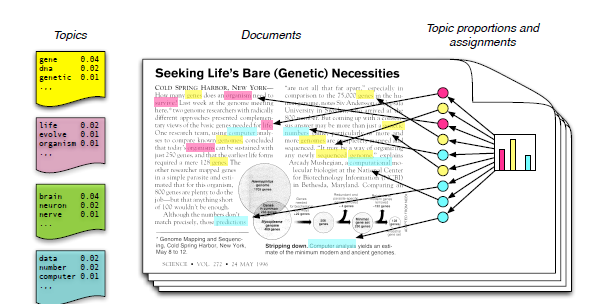
\includegraphics[scale=0.9]{./Slike/slika1.png} 
	\caption{Пример чланка, преузето са \cite{blei1}}
	\label{fig:slika1}
\end{figure}

На левој стани слике дате су неке теме ( енг. \textit{Topics}) које са одређеним вероватноћама садрже неке речи. На основу припадности речи темама, извршава се описани процес означавања ("бојења") речи да би се на крају добили удели тема у тексту ( десна страна слике, енг. \textit{Topics })
Важно је приметити да у тексту постоји доста речи које не одређују ни једну конкретну тему и које се са готово истим, малим вероватноћама могу сврстати у сваку од њих. Такве речи су нпр. везници, личне заменице ,прилошке одредбе итд. Оне се једним именом називају енг. \textit{stop words}. Како присуство таквих речи не утиче на тематику документа, то их при математичкој анализи текста треба занемарити.  



LDA је статистички модел који формално описује описани процес означавања речи. Да би се у потпуности разумело како LDA ради, потребно је упознати се са   \textit{генеративним процесом} -  процесом којим се креирају документи са становишта LDA-a.

\subsection{Генеративни процес}
Нека је дат неки скуп речи најчешће коришћених у научним областима математике, физике, хемије, музике, рачунарства и биологије. Нека је, даље, потребно креирати документ који има одређен број речи из датог скупа речи али тако да он највише "говори о"  математици и музици, али поред ових тема, у мањој мери, "говори о" физици и програмирању, док се остале теме занемарљиво мало помињу.
Како је дат фиксан скуп речи - речник (вокабулар ), могуће је свакој речи придружити \textit{вероватноћу} припадања свакој од тема. Тако ће на пример реч \textit{интеграл} имати велике вероватноће припадања темама математика и физика, мање вероватноће у темама хемија и рачунарство док ће се са јако малим вероватноћама јављати у осталим темама. Дакле, једна реч припада свакој од датих тема али са различитим вероватноћама. 

Генерисање траженог документа могуће је извести следећом процедуром :

\begin{enumerate}
 \item Одабрати расподелу тема у документу - прецизирати која тема се са којим уделом појављује у документу. У конкретном примеру, расподела би могла бити : математика 30\%, музика 30\%, физика 20\%,програмирање 15\%, биологија 2\% и хемија 3\%.
 \item Докле год није достигнут тражени број речи
 	\begin{enumerate}
	\item Изабрати тему из дистрибуције која је одабрана у 1.
	\item Изабрати реч из теме која је одабрана у 2.а). Како свака тема има речи које фаворизује ( веће вероватноће у односу на остале речи ), то ће се те речи највероватније одабрати у овом кораку.
	\end{enumerate}

 \end{enumerate}

Описана процедура може се графички илустровати претходном сликом (~\ref{fig:slika1}). Одабрана расподела тема у документу ( тачка 1 описане процедуре) предсављена је хистограмом на десној страни слике. Обојени кругови представљају одабир теме из документа ( корак 2.а) ) док речи повезане стралицама са њима представљају одабирану реч из те теме ( корак 2.б) ).\footnote{Расподела на основу које се одабирају пропорције тема у кораку 1, назива се Дирихлеова раподела, енг. Dirichlet distribution. На основу те одабране расподеле, врши се придруживање речи документима, енг. allocate } 

Формално, тема се дефинише као расподела речи над неким фиксним скупом речи - речником. Рецимо, тема биологија ће са већом вероватноћом садржати речи везане за ту област нпр. биљка, животиња, ћелија, ген итд. док ће тема везана за математику ове речи садржати са нижим вероватноћама у односу на речи нпр. број, разломак, променљива,коцка итд.


%PROVERI JOS JEDNOM DA LI MOZE TAKO DA SE KAZE

Дакле, основна карактеристика LDA-a је то што сви документи деле \textbf{исти скуп тема} али сваки документ те теме садржи у различитим односима. Овакаво посматрање докумената јако је природно и интуитивно.%{\color{red} Уколико би се могао формирати скуп свих речи које познаје нека особа, а затим тај скуп поделити по темама која та особа уме да разликује, механизам којим ће та особа препознати тематику докумената је у ствари начин на који LDA ради.} PROVERI!!!!

\subsection{Како се откривају теме - упрошћен пример }

Проликом генерисања поменутог документа, било је познато која тема садржи које речи као и у којим односима је заступљена свака тема у тексту. Циљ алгоритама за моделовање тема је да \textbf{аутоматски} "открије"  које су то теме присутне у неком документу и које речи припадају којој теми али \textbf{само} на основу речи које се јављају у документу, без било каквог додатног знања.
Сазнање о томе која тема се у којој мери налази у неком документу, није од превеликог практичног значаја. Међутим, уколико је на располагању огромна количина докумената ( нпр. дигитална база свих издаља листа "Политика" ), откривање сродних докумената, или докумената који се баве само одређеним темама може бити јако важно. Због тога ће се надаље говорити о скупу докумената над којим се извршава моделовање тема, уместо о једном документу. Притом, наравно, и даље важи претпоставка да сваки документ "говори о"   свим темама које се могу издвојити из свих докумената, само у различитим односима.

Према свему реченом, једино што је \textit{видљиво}, енг. \textbf{\textit{observed}} су документи, односно речи које се у документима јављају.  Тематска расподела по документима, као и расподела речи по темама су \textbf{\textit{скривене или невиљиве}}, енг.\textit{non observed,hidden} (Слика \ref{fig:slika2})

\begin{figure}[H]
    \centering
   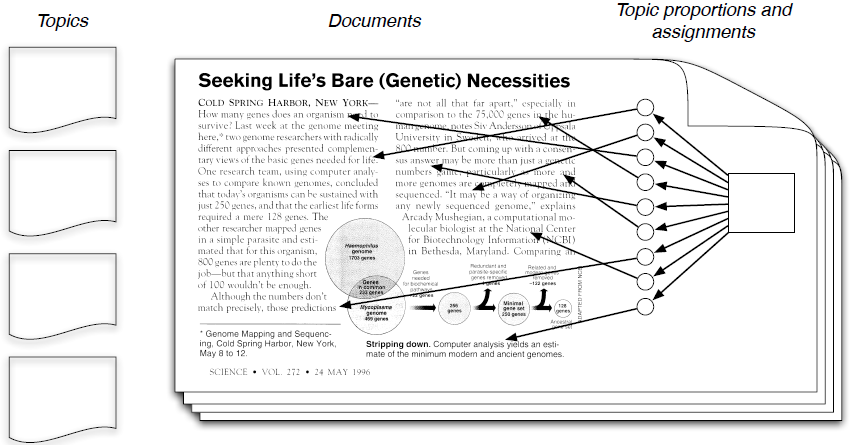
\includegraphics[scale=0.5]{./Slike/slika2.png} 
	\caption{Пример чланка, преузето са \cite{blei2}}
	\label{fig:slika2}
\end{figure}

Основни задатак алгоритма је окривање скривених структура на основу видљивих. У овом тренутку, моделовање тема можемо посматрати као \textbf{обрнути} генеративни процес. Дакле, циљ моделовања тема је откривање скривених структура из којих су \textbf{највероватније}, генеративним процесом, добијени видљиве структуре, тј. документи. Током рада, откривају се удели различитих тема по документима као и расподеле речи унутар тема.
Важно је напоменути да \textbf{именовање} тема не постоји у основној верзији алгоритма. Алгоритам групише речи у одређене целине - теме, а насловљавање тема се препушта стручњацима.




Нека је дат једноставан документ који, након склањања везника, личних заменица и осталих шумова (енг.\textit{stopwords}) садржи речи приказане у следећој табели.

\begin{figure}[H]
    \centering
   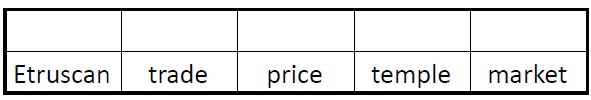
\includegraphics[scale=0.8]{./Slike/slika3.png} 
	\caption{Преузето са \cite{mimno1}}
	\label{fig:slika3}
\end{figure}

Процес моделовања тема започоње \textbf{случајним додељивањем} тема свакој од речи у документу. Дакле, пошто не постоји никакво знање о присуству тема у документима као ни о томе која реч припада којој теми, ову доделу је неопходно урадити на случајан начин. Интуитивно је јасно да се за тако нешто унапред мора одредити број тема који се захтева у задатом скупу докумената. Више о улазним параметрима алгоритма може се наћу у одељку 3 овог рада.
Пример једне случајне доделе дат је на следећој слици .
\begin{figure}[H]
    \centering
   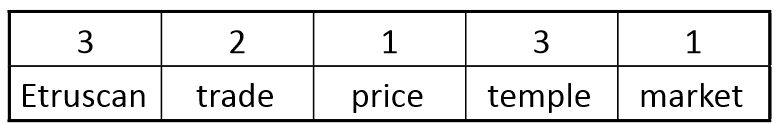
\includegraphics[scale=0.6]{./Slike/slika4.png} 
	\caption{Преузето са \cite{mimno1}}
	\label{fig:slika4}
\end{figure}

На овај начин је направљена иницијална \textbf{расподела} тема унутар посматраног документа - 40\% текста говори о теми 3, 40\% о теми 1, док 20\% говори о теми 2.

Уколико сада на сличан начин доделимо теме и осталим документима, полазни скуп докумената може се приказати следећом сликом.

\begin{figure}[H]
    \centering
   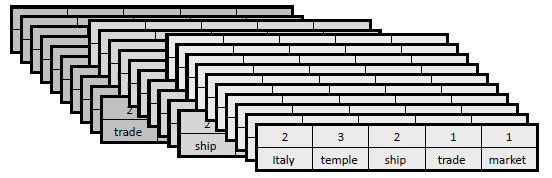
\includegraphics[scale=0.6]{./Slike/slika5.png} 
	\caption{Преузето са \cite{mimno1}}
	\label{fig:slika5}
\end{figure}

Пошто сваки документ има иницијалну, \textbf{случајну} расподелу тема, једноставно је груписати речи унутар тема и на тај начин направити иницијалну \textbf{случајну} расподелу речи по темама. Одређивање расподеле по темама, може се илустровати следећом сликом.


\begin{figure}[H]
    \centering
   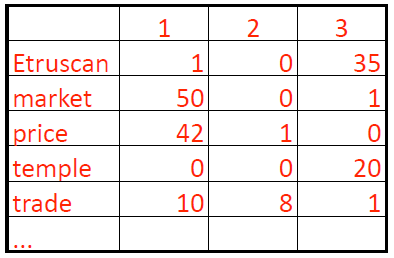
\includegraphics[scale=0.6]{./Slike/slika6.png} 
	\caption{Преузето са \cite{mimno1}}
	\label{fig:slika6}
\end{figure}
У првој колони табеле уписане су све речи из свих докумената (речник ) док је затим у свакој од наредних колона уписан одговарајући број који означава колико пута је дата реч додељена тој теми. Рецимо, бројеви 1 0 35 у другој врсти табеле означавају да је реч \textit{Etruscan} 35 пута била сврстана у тему број 3, једном је била додељена теми број 1 док се ниједним није нашла у теми број 2..
Дакле, почевши од друге колоне приказане табеле, табела по колонама, садржи  \textit{расподелу речи по темама}. Једноставним сортирањем колона, добијају се највероватније речи у свакој од тема.

У овом тренутку, расподеле које су добијене нису релевантне зато што у позадини стоји апсолутно случајно додељивање тема које није базирано на документима, тј. на јединим видљивим подацима.
Дакле, потребно је добијене резулатате \textit{прилагодити} тако да осликавају тематску структуру документа. Прилагођавање се одвија у одређеном, унапред познатом броју итерација. Генерално, што је већи број итерација, то су добијене расподеле релевантније, мада, како резултати показују, постоје и нека ограничења за ове вредности. Више о одређивању оптималног броја итерације може се наћи у одељцима 3 и 6 овог рада.

Унутар једне итерације, за сваки документ  за сваку реч унутар тог документа врши се провера колико је тренутно додељена тема адекватна, тј. да ли постоји боља тема којој би та реч могла бити додељена. На тај начин, из итерације у итерацију, расподеле све више и више осликавају структуру докумената.

Нека је почетна расподела по темама дата на претходним сликама (\ref{fig:slika5},\ref{fig:slika6}). Нека се провера подобности теме прво извршава за реч \textit{trade} првог документа. Ова реч је унутар првог документа додељена теми број 2, док је, гледано са становишта свих докумената који се посматтају, укупно 8 пута сврстана у ту тему. Потребно је испитати да ли тема број 2 највише одговара тој речи.
Претпоставимо да знамо теме за све остале речи, како из документа који се посматра, тако и за остале документе, и да је једино непозанто којој теми припада \textit{trade}  у посматраном документу.
Дакле, расподела тема у посматраном документу као и расподела речи по темама, сада изгледа као на следећој слици и потребно је доделити изабраној речи тему унутар посматраног документа.

\begin{figure}[H]
    \centering
   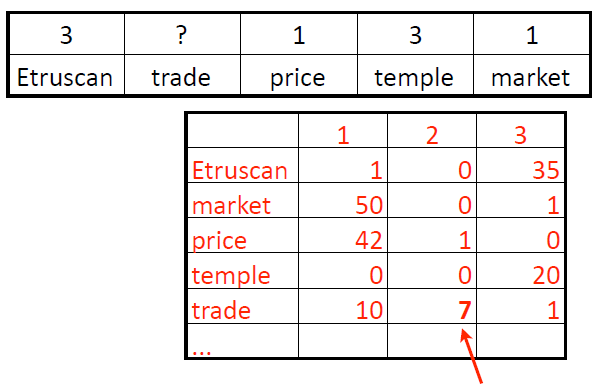
\includegraphics[scale=0.6]{./Slike/slika7.png} 
	\caption{Преузето са \cite{mimno1}}
	\label{fig:slika7}
\end{figure}

Уколико се посматра расподела тема у изабраном документу, приметиће се да документ највише "говори о"  темама 3 и 1 док о теми 2 не говори уопште. Према томе, удели тема 3 и 1 су значајни, док је удео теме 2 занемарљиво мали. Обзиром да је основна претпоставка овог модела да сви документи говоре о свим темама, не може се рећи да изабрани документ уопше "не говори" о теми 2. Начин на који ће се означити да је тема 2 јако слабо присутна у изабраном документу врши  се тако што се теми 2 додели јако мали удео. Обизиром да је у питању реч из документа који има неки одређену расподелиу тема, логично је очекивати да избор теме за ту реч зависи од тема тог документа.

Удели тема у изабраном документу могу се представити дужином линија, као што је приказано на следећој слици.


\begin{figure}[H]
    \centering
   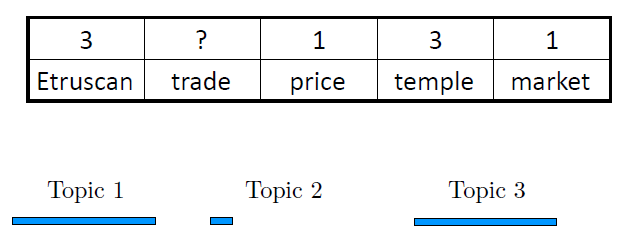
\includegraphics[scale=0.6]{./Slike/slika8.png} 
	\caption{Преузето са \cite{mimno1}}
	\label{fig:slika8}
\end{figure}

Међутим, како је речник ( скуп речи) заједнички за све документе, тема речи зависи и од глобалног присуства те речи у свим темама. И ова претпоставка је логична, јер, као што је на почетку наведено, свака реч припада свим темама, само са различитим верпватноћама. Глобално присуство изабране речи у свим темама приказано је на следећој слици :

\begin{figure}[H]
    \centering
   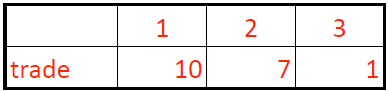
\includegraphics[scale=0.6]{./Slike/slika9.png} 
	\caption{Преузето са \cite{mimno1}}
	\label{fig:slika9}
\end{figure}


Дакле, избор теме за реч \textit{trade}  зависи од расподеле тема у посматраном документу као и од присуства те речи у свим темама. Ова зависност може се представити следећом сликом :

\begin{figure}[H]
    \centering
   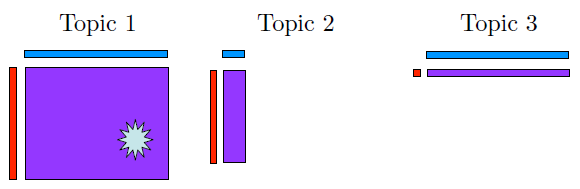
\includegraphics[scale=0.6]{./Slike/slika10.png} 
	\caption{Преузето са \cite{mimno1}}
	\label{fig:slika10}
\end{figure}

Вертикална, црвена линија представља присуство речи у одговарајучој теми ( формалније, вероватноћу са којом се та реч налази у изабраној теми ). Љубичаста "површина" представља подобност да одговарајућа тема буде додељена тој речи у изабраном документу. Како се слике јасно може уочити, "највећу"  површину формира тема 1 те је, према томе, речи  \textit{trade} додељује тема број 1 у овој итерацији. Након извршене измене, расподела тема у документу, као и расподела речи по темама, приказана је на следећој слици :



\begin{figure}[H]
    \centering
   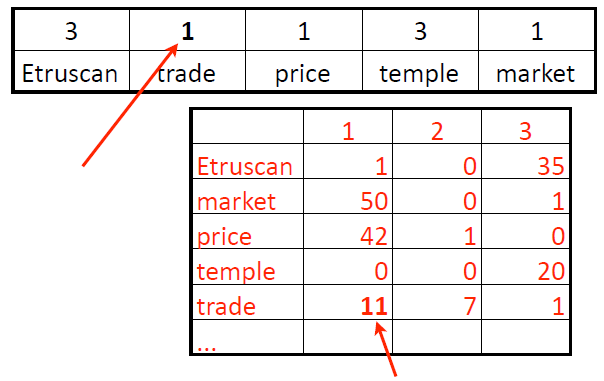
\includegraphics[scale=0.6]{./Slike/slika11.png} 
	\caption{Преузето са \cite{mimno1}}
	\label{fig:slika11}
\end{figure}


На овај начин, избараној речи додељена је најверпватнија тема а тематска слика документа "више личи" на реалну слику. 

Ако се описани процес примени на сваку реч сваког документа, расподеле ће из итерације у итерацију све више осликавати структуру полазних докумената. Обзиром да избор теме за сваку реч зависи од тренутно додљених расподела тема и речи, овим процесом се узимају у обзир видљиви подаци. Дакле, скривене структуре ( непознате расподеле) се генеришу на основу једино видљивих података - докумената и речи у њима.

Узевши све претходно у обзир, јасно је због чека не постоји именовање тема. Када се процес "генерисања"   заврши ( нпр. достигне  одређени број итерација ), сортирањем одговарајућих колона из табеле са слике \ref{fig:slika7}, добија се  расподела речи по темама. На основу експретског знања овим расподелама додељују се имена - нпр. тема 1 - математика, тема 2- економија итд.

\subsection{Графички пример моделовања тема}

Алгоритми за моделовање тема, поред текста, могу се применити и на друге облике података. Једна од могућих примена је и "октирвање тематике" слика. Рецимо, помоћу ове групе алгоритама могуће је препознати "сличне" слике. Овај рад неће се бавити овом врстом примене, али се  ТМ алгоритама може јако добро илустровати једноставним графичким примером. Ради бољег разумевања шта ТМ уствари ради, биће описан један  пример примене ТМ над сликама.


%Нека је дат скуп једноставних слика, као што је приказано на 



























\chapter{Математичка позадина}


У претходним поглављима, рад се углавном бавио питањима \textit{шта је ТМ алгоритам и чему  служи}, без улажења у то \textit{\textbf{како}} он уствари ради. 

Опис рада ТМ алгоритама - конкретно LDA имплементације, биће изложен у неколико целина. Најпре ће се објаснити ( увести ) неки  појмови вероватноће који су битни за разумевање сусштине рада алгоритма, а затим ће  бити изнешена математичка позадина самог алгоритма.

\section{Теорија вероватноће}

Теорија вероватноће је математичка дисциплина која се бави изучавањем случајних појава тј. појава чији исходи нису увек строго дефинисани.

Први проблеми који се могу сматрати проблемима вероватноће потичу још из 12. века и везани су за проучавање исхода разних игара на срећу.  Развој \textit{теорије вероватноће} почиње средином 17. века и везан је за имена Блеза Паскала,Пјера де Ферма и Кристијана Хајгенса. Наиме, између Паскала и Ферма је 1654. године започела интересантна преписка о низи проблема међу којима је био и проблем везан за поделу улога приликом прекида једне коцкарске игре. Проблем је био постављен на следеђи начин : Два играча А и Б се договоре да читав улог припадне ономе ко први добије три игре. Када је играч А добио 2 игре а играч Б једну игру, играчи су споразумно одлучили да прекину игру. Поставља се питање како сада да поделе улог. Паскал је предложио поделу у односу 3:1 у корист играча А.
Овај пример често се узима као почетак настанка теорије вероватноће.

Неке од појава које се догађају у реалном свету лако се могу предвидети и објаснити услод познавања законитости њиховог настанка. У такве појаве спадају нпр. помарачење Сунца и Месеца, плима и осека, гравитација итд.
Међутим, постоје појаве чије узроке тренутно није могуће одредити па се не могу у потпуности објаснити и одредити. Неке од таквих појава су нпр. добитак на лутрији или метереолошке појаве.
Прилоком бацања металног, хомогеног новчића, никада није сигрно да ли ће пасти писмо или глава. Међутим, уколико бацамамо новчић много пута, може се уочити да је отприлике исти број пута пало писмо као и глава ( такве експерименте су радили Буфон и Пирсон% - референце! ).
Дакле, законитост код оваквих догађаја може се уочити тек након великог броја понаваљања појаве.

\subsection{Основни појмови}


Основни полазни појам у теорији вероватноће је непразан скуп $\Omega$ који представља скуп свих могућих исхода једног експеримента. Овај скуп се често назива \textbf{простор елементарних догађаја} и може бити коначан, пребројив или непребројив. 
\textbf{Случајни догађаја} или само \textbf{догађај} представља било који подскуп скупа $\Omega$. Најчешће се случајни догађаји означавају великим, штампаним, латиничним словима. За догађај \textbf{А} каже се да се \textbf{реализовао} ако се реализовао неки исход $\omega$ који припада скупу А. Догађај који је садржи све могуће елементарне исходе експеримента назива се \textbf{сигуран догађај} а догађај који не садржи ни један елементарни исход назова се \textbf{немогућ догађај}.


\textit{Пример:}
Нека је дата хомогена коцка чије су стране означене бројевима од 1 до 6. Елементарни догађаји су појављивање одређеног броја при бацању коцкице. Према томе, скуп свих могућих исхода екперимента бацања коцкице је $ \Omega = \lbrace 1,2,3,4,5,6 \rbrace $. Догађај A = "пао је паран број" одређује скуп $ $А$ = \lbrace 2,4,6 \rbrace $


\textbf{Производ два догађаја} $ А $ и $ В $, у ознаци $ AB $ је догађај који се реализује ако и само се ако реализују оба догађаја. Дакле, производ догађаја је пресек скупова А и В. Уколико су А и В дисјунктни скупови (пресек је празан скуп) за такве догађаје кажемо да су \textbf{несагласни} или да се \textbf{искључују}.

\textbf{Збир два додгађаја} А и В, у ознаци $ A \cup B $ представља догађај који се реализује ако се реализује бар један од догађаја А и В. 

\textbf{Разликом догађаја} А и В, у ознаци $ A -  B $ назива се догађај који се реализује ако и само ако се реализује догађај А  а не реализује догађај В. 

\textbf{Потпун систем догађаја} : За догађаје $ A_1,A_2,..A_n$ се каже да образују \textit{потпун систем догађаја} уколико важи : $ \bigcup_{i} A_i = \Omega $ . Дакле, при реализацији неког експеримента бар један од догађаја $ A_1,A_2,..A_n$ ће се реализовати. Посебно су интересантни потпуни системи несагласних догађаја као што се може видети код формуле тоталне вероватноће.

\begin{de}
[Класична дефиниција вероватноће] : Нека је $ \Omega = \lbrace \omega_1,\omega_2,...,\omega_n \rbrace $ скуп свих могућих једнаковероватних елементарних догађа који су међусобно несагласни и нека је $ A = \lbrace \omega_{i_1}, \omega_{i_2}, ... , \omega_{i_m} \rbrace $ догађај који се састоји од \textit{m} елементарних једнаковероватних догађаја. Вероватноћа наступања догађаја А је :
\begin{equation}
 P(A) = \frac{m}{n} 
\end{equation}
\end{de}

 Претходна дефиниција може се неформално изразити и овако : вероватноћа догађаја A једнака је количнику броја \textbf{повољних исхода} експеримена ( исходи када се реализује догађај А ) и укупног броја свих могућих исхода експеримента.

Класична дефиниција вероватноће је применљива само онде где су елементарни догађаји једнаковероватни. Међутим, тај услов је у пракси јако тешко испунити. Чак и у случајевима када је то наизглед очигледно, као што је бацање коцкице, једнаковероватност не може бити гарантована.  Разлози за то могу бити технологија израде коцкице која не мора бити савршено прецизна, немогућност обезбеђивања идеалних и непромењљивих услова током извођења експеримента итд. Због тога је једини начин којим је могуће заиста утврдити вероватноћу догађаја А \textit{статистички приступ} заснован на великом броју експеримената.




\begin{de}
[Статистичка дефиниција вероватноће] : 
Нека се  у $n$ понављања експеримента изведених под приближно истим условима догађај А реализовао ${m_n}$ пута. Вероватноћа догађаја А је
\begin{equation}
 P(A) = \lim_{n\to\infty}\frac{m_n}{n} 
\end{equation}
\end{de}

\subsection{Условна вероватноћа}

Вероватноћа догађаја чија реализација \textbf{не зависи} од наступања било ког другог догађаја назива се \textbf{безусловна вероватноћа}. Ако је реализација догађаја А условљена реализацијом неког догађаја В при чему В није немогућ догађај ( $ P(B) \neq 0 $), тада се вероватноћа догађаја под условом да се десио догађај В назива \textbf{условном вероватноћом} и означава се са 
$ P(A \mid B )$. Дакле, $ P(A \mid B )$ је вероватноћа догађаја А под условима који сигурно доводе до реализације догађаја В.

Нека се изводи експеримент у коме постоји $n$ једнаковероватних елементарних догађаја и нека је са $n_A,n_B,n_{AB}$ означен број елеменгтарних догађаја који доводе до реализације догађаја $A, B ,AB$ редом. 

Према класничној дефиницији вероватноће, вероватноћа реализације догађаја А и АВ је :
\begin{equation}
P(B) = \frac{n_B}{n}, P(AB) = \frac{n_{AB}}{n}
\end{equation}
Ако је реализација догађаја А условљена реализацијом догађаја В, то је број повољних исхода догађаја А $n_{AB}$ (број елементарних догађаја који имају осбине и скупа А и скупа В ). Пошто се догађај А реализује само ако се реализовао догађај В, број свих могућих исхода је $n_B$ (број свих могућих елементарних догађаја када наступа догађај В). Дакле, условна вероватноћа догађаја А, под условом да се десио догађај В је :

\begin{equation}
 P( A \mid B ) = \frac{n_{AB}}{n_B} = \frac{\frac{n_{AB}}{n}}{\frac{n_B}{n}} = \frac{P(AB)}{P(B)} \quad ,  P(B) \neq 0
\end{equation}

У случају да је догађај В условљен догађајом А, аналогно се изводи да је 

\begin{equation}
 P( B \mid A ) = \frac{P(AB)}{P(A)} \quad ,  P(A) \neq 0
\end{equation}

Из релација (3.4) и (3.5) следи

\begin{equation}
 P( AB ) = P(B)\cdot  P( A \mid B ) = P(A)\cdot  P( B \mid A ) 
\end{equation}

Релација (3.6) назива се још и \textbf{теорема о производу вероватноћа}

\begin{te}
[Формула тоталне вероватноће] : 
Ако су $H_1,H_2,..,H_n$ међусобно несагласни догађаји, $P(H_i) > 0 (i=1,..,n)$ при чему важи $H_1+H_2+..+H_n = \Omega $ тада је :
\begin{equation}
	 P(A) = \sum_{i=1}^n P(H_i)P(A \mid H_i)  \textrm{ за сваки догађај}  A \subseteq  \Omega 
\end{equation}
\end{te}
Напомена : Догађаји $H_1,H_2,..,H_n$ чине потпун систем несагласних догађаја.

\begin{dok}
Обзором да су догађаји подскупови скупа свих елементарних догађаја очигледно је да важи

\begin{equation}
A = A\Omega = A \sum_{i=1}^n H_i = \sum_{i=1}^n AH_i. 
\end{equation}
На основу релације (3.6) следи :

\begin{equation}
P(A) = P(\sum_{i=1}^n AH_i) = \sum_{i=1}^n P(AH_i) = \sum_{i=1}^n P(H_i)P(A \mid H_i)
\end{equation}
\end{dok}

Вероватноће $P(H_i)$ су обично познате унапред и називају се \textbf{априорним вероватноћама} а сами догађаји \textbf{хипотезама}. 

\begin{te}
[Бајесова формула \footnote{енг. Bayes} ] : 
Ако су $H_1,H_2,..,H_n$ међусобно несагласни догађаји, $P(H_i) > 0        (i=1,..,n)$ при чему важи $H_1+H_2+..+H_n = \Omega $ тада је :
\begin{equation}
	 P(H_i \mid A ) = \frac{P(H_i)P(A \mid H_i)}{ \sum_{j=1}^n P(H_j)P(A \mid H_j)}  \quad   (i=1...n)  \quad  \textrm{ за сваки догађај}  A \subseteq  \Omega 
\end{equation}
\end{te}

\begin{dok}
Из релације (3.6) следи :

\begin{equation}
P(H_iA) = P(H_i)P(A \mid H_i) = P(A)P(H_i \mid A) \quad  (i=1...n)
\end{equation}
Условна вероватноћа догађаја $H_i$ под условом да се десио догађај А је:
$$ P(H_i \mid A) = \frac{P(H_iA)}{P(A)} = \frac{P(H_i)P(A \mid H_i) }{P(A)} $$

Примењујући формулу потпуне вероватноће за $P(A)$  добија се 
$$
 P(H_i \mid A ) = \frac{P(H_i)P(A \mid H_i)}{ \sum_{j=1}^n P(H_j)P(A \mid H_j)}
$$
што представља Бајесову формулу.

\end{dok}

\subsection{Случајне променљиве}

Ако се сваком елементарном догађају придружи један реалан број, онда се извођење експеримента може посматрати као избор вредности једне променљиве. Променљива величина која 
 те бројене вредности узима са одређеним вероватноћама назива се \textit{случајна променљива}. Дакле, уместо вербалне карактеризације догађаја ( описа речима шта догађај представља ) много је једноставније за рад догађаје окарактерисати бројним вредностима тј. неким реалним бројевима.

\textit{Пример 1 :} У екпериманту бацања новчића могућа су два елементарна исхода : грб или писмо. Нека је догађај који се посматра "пало је писмо". Појава писма се може означити бројем 1 а појава грба бројем 0. Сада се овај екперимент може замислити као избор 0 или 1 са вероватноћом $\frac{1}{2}$

\textit{Пример 2 :} Новчић се баца два пута. Нека је са P означена појава писма а са G појава грба. Скуп свих елементарних исхода екперимента је $ \Omega = \lbrace PP,PG,GP,PP \rbrace$ . Нека је догађај који се посматра "број палих писама". Сваком исходу се може доделити један реалан број и то $ PP -> 2, GP -> 1,PG -> 1, GG ->0$. Ово додељивање вредности се карактерише случајном променљивом.  Случајна променљива сваку од ових вредности узима са различитом вероватнићом.  

\begin{figure}[H]
    \centering
   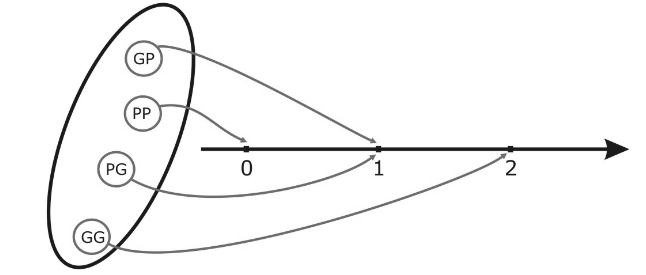
\includegraphics[scale=0.5]{./Slike/slika12.png} 
	\caption{Графички пример случајне променљиве}
	\label{fig:slika12}
\end{figure}

\begin{de}
Функција Х која сваком случајном догађају $\omega \in \Omega $ додељује неки реалан број $X(\omega)$ назива се \textbf{случајна променљива} где је $X:\Omega \longrightarrow R $
\end{de}

Дакле, случајна променљива је пресликавање скупа $\Omega $ у скуп \textbf{реалних} бројева за разлику од вероватноће која је пресликавање скупа  
$\Omega $ у скуп $ [0,1]$

Важно је уочити да случајна променљива \textbf{нема конкретну вредност} већ се само говори о вероватноћама да узме неки конкретну вредност.

Разликују се два основна типа случајних променљивих - \textbf{дискретне} и \textbf{непрекидне}. Подела се врши у зависности од тога да ли случајна променљива узима вредности у пребројивом или непребројивом скупу вредности.



\subsubsection{Дискретне случајне променљиве}

За случајну променљиву се каже да је дискретног типа ако узима коначан број изолованих вредности или пребројиво много вредности

\begin{de}
Нека случајна променљива Х може да узме вредности $x_1,x_2, ... , x_n$ са вероватноћама $p_1,p_2, ... ,p_n$ при чему важи да је $p_1 + p_2 + ... + p_n = 1$. Скуп парова $(x_i,p_i = P\lbrace X=x_i \rbrace), i=1,2,...,n$ или написано :
$$ 
\left(
\begin{array}{ccc}
x_1 & x_2 & \cdots \\
p(x_1) & p(x_2) & \cdots \\
\end{array}
\right)
$$

чине закон расподеле  или распоред вероватноћа случајне променљиве Х.
\end{de}

\textit{Закон расподеле случајне промнљиве} може да се посматра као \textbf{правило} по коме се свакој вредности случајне променљиве придружује одговарајућа вероватноћа. Дакле, при реализацији експеримента сигурно ће се десити догађај којем је придужена нека вредност случајне променљиве. Због тога је сума свих вероватноћа у расподели случајне променљиве 1. Међутим, нису све вредности подједнако вероватне па се свакој вредноти придружује вероватноћа са којом се очекује.
Претходна дефиниција може се интерпретирати и на следећи начин : извесна маса једнака јединици је распоређена на такав начин да се у тачкама $x_1,x_2, ... , x_n$ налазе одговарајући делови масе $p_1,p_2, ... ,p_n$. Услед оваквог тумачења, закон расподеле вероватноћа се често назива и \textbf{функција масе вероватноћа}

У примеру 2, случајна променљива може да узме три вредности, тј. писмо се може појавити 0,1 или 2 пута у два бацања. Ни један други исход није могућ - нпр. у два бацања писмо не може да се појави 3 пута или -1 пут. Међутим, вероватноћа да се писмо неће појавити ни једном (или да се појави два пута) је $\frac{1}{4}$ - вероватноћа да падне глава у првом бацању је $\frac{1}{2}$ и вероватноћа да падне глава у другом бацању је   $\frac{1}{2}$, дакле, вероватноћа да оба пута падне глава је је  $\frac{1}{2} \cdot \frac{1}{2} = \frac{1}{4}$, вероватноћа да се писмо појави тачно једном је $\frac{1}{2}$ - писмо пада тачно једном у случају PG или GP. Вероватноћа за оба ова догађаја је $\frac{1}{4}$. Дакле, вероватноћа да се десио бар један од ових догађаја је  $\frac{1}{4} + \frac{1}{4} = \frac{1}{2}$. Према томе, расподела случајне променљиве "број појављивања писма у два бацања " је :


$$ 
\left(
\begin{array}{ccc}
0 & 1 & 2 \\
\frac{1}{4} & \frac{1}{2} & \frac{1}{4} \\
\end{array}
\right)
$$

Закон расподеле дискретне случајне променљиве може се представити графички, као на следећој слици :

\begin{figure}[H]
    \centering
   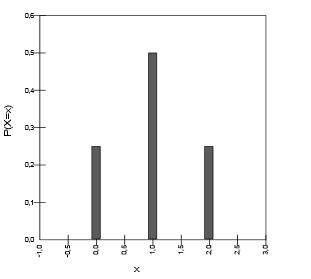
\includegraphics[scale=0.8]{./Slike/slika13.png} 
	\caption{Графички пример случајне променљиве}
	\label{fig:slika13}
\end{figure}

На апсциси се налазе могуће вредности случајних променљивих док се на ординати налазе вероватноће са којом случајна променљива узима дату вредности. Са претходне слике јасно се уочава дискретност посматране случајне променљиве - вероватноћа да случајна промељива узме вредност између неке две целобројне вредности је 0. 
\\
\\

\textbf{Функција расподеле дискретне случајне 
променљиве:}
\\

Распоред или закон расподеле случајне променљиве дискретног типа може се представити као листа свих могућих вредности случајне променљиве и одговарајућих вероватноћа. Међутим, поставља се питање како представти случајну променљиву која може узимати јако пуно вредности тј. бесконачно много вредности. У овом случају би требало формирати листу од бесконачно много чланова, што је практино неизводљиво. (Пример једне такве случајне променљиве би био - број бацања коцкице док се не добију две узастопне шестице. Случајна променљива може узети вредности 2,3,4,... са различитим вероватноћама, при чему не постоји горња граница броја бацања при којој се сигурно добијају две узастопне шестице ).
Због описаног проблема, потребно је пронаћи другачији начин представљања случајне променљиве и одговарајућих вероватноћа. То се постиже \textbf{функцијом расподеле} која се може дефинисати за сваку случајну променљиву.

\begin{de}
\textbf{Функција расподеле} ( још се назива и \textbf{кумулативна функција расподеле}) дискретне случајне променљиве претставља вероватноћу да случајна променљива Х узме вредност која је мања или једнака неком реалном броју $x$ при чему је дефинисана за свако реално   $x$. 
$$ F(x) = P (X<x) \quad \forall x \in R $$
\end{de}

Дакле, кумулативна функција расподеле има облик

$$
F(x) = \left\lbrace
\begin{array}{rl}
0, & x \leq x_1 \\
p_1, & x_1 < x \leq x_2 \\
p_1 + p_2, & x_2 < x \leq x_3 \\
.... & ... \\
1 & x > x_n
\end{array}
\right.
$$

и може се изразити као :

$$
F(x) = \sum_{k,x_k<x} P(X = x_k)
$$

а графички приказ је дат на следећој слици :


\begin{figure}[H]
    \centering
\captionsetup{justification=centering}
   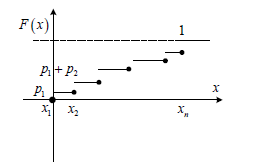
\includegraphics[scale=0.8]{./Slike/slika14.png} 
	\caption{График кумулативне функције расподеле \\ случајне променљиве дискретног типа} 
	\label{fig:slika13}
\end{figure}

Две најважније дискретне расподеле су \textbf{Биномна} и \textbf{Пуасонова} расподела.

\subsubsection{Непрекидне случајне променљиве}
Случајна променљива је (апсолутно) непрекидног типа ако може да узме \textbf{било коју } вредност из неког интервала. Број вредности које може да узме случајна променљива непрекидног типа је \textbf{бесконачан}. Неки од примера су : висина и тежина људи, дужина трајања батерије итд.
На пример, нека је Х случајна променљива која представља дужину рада сијалице. Ова случајна променљива може узети било коју вредност на интервалу од 1 до нпр. 1000 сати. Како у интервалу $[0,1000]$ има бесконачно много реалних бројева, не постоји начин да се дефинише вероватноћа за сваку појединачну вредност, као што је био случај код дискретних променљивих. Такође, интуитивно је јасно да је вероватноћа да ће сијалица прегорети у тачно одређеном тренутку једнака 0  док је вероватноћа да ће прегорети у неком временском интервалу различита од нуле.


\begin{de}
Случајна променљива X је апсолутно непрекидног типа ако постоји \textbf{ненегативна} функција $ f: \mathbb{R} -> \mathbb{R}$ таква да за било који интервал $[a,b] \subset (- \infty,\infty)$ важи :
\begin{equation}
P \lbrace a \leq X < b \rbrace = \int\limits_{a}^{b} f(x)dx
\end{equation}
\end{de}

Функција $f(x)$ мора да задовољи услов : 
$$
P \lbrace - \infty \leq X <  \infty \rbrace = P \lbrace \Omega \rbrace =  \int\limits_{- \infty}^{\infty} f(x)dx  = 1
$$

Функција $f(x)$ се назива \textbf{густина расподеле вероватноће} случајне променљиве Х.
Случјане променљиве \textbf{дискретног типа } немају густину расподеле баш као што ни случајне променљиве непрекидног типа немају закон расподеле вероватноћа.

Из релације (3.12) следи да је вероватноћа да случајна променљива узме вредност из интервала  $[a,b]$ једнака \textbf{површини} испод графика функције $f(x)$ на интервалу $[a,b]$.




\begin{figure}[H]
    \centering
\captionsetup{justification=centering}
   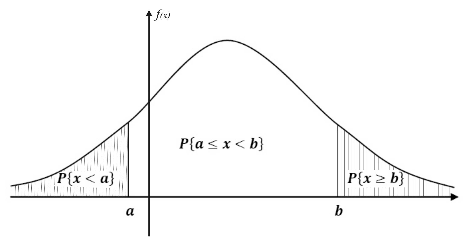
\includegraphics[scale=0.8]{./Slike/slika15.png} 
	\caption{Функција густине} 
	\label{fig:slika13}
\end{figure}


\textbf{Функција расподеле непрекидне случајне 
променљиве:}



\begin{de}
\textbf{Функција расподеле} (\textbf{кумулативна функција расподеле}) непрекидне случајне променљиве се може представити као :

$$
F(x) = P (X \leq x) = \int \limits_{-\infty}^{x} f(t)dt) \quad x \in (-\infty,\infty) 
$$
где је $f(x)$ функција густине.
\end{de}

Дефиниција кумулативне суме  преко интеграла је јаснија ако се има на уму интервал из ког случајна променљива може да узме вредности. Код случајних променљивих дискретног типа, тај скуп је био пребројив па се кумулативна функција расподеле дефинисала преко суме. Случајне променљиве непрекидног типа могу узти бесконачно много вредности па се сума код дискретних случајних променљивих ( када број тачака тежи у бесконачност) замењује интегралом.

Напомена : Ако случајна променљива Х не узима све вредности из интервала $ (-\infty,\infty) $ усваја се да је $f(x) = 0$ за све вредносто $x$ из интервала у којима Х не узима вредности.

График кумулативне функције расподеле непрекидне случајне променљиве Х је сада представљен глатком кривом линијом ( за разлику од случајне променљиве дискретног типа где је график био "степенаст" ).


\begin{figure}[H]
    \centering
\captionsetup{justification=centering}
   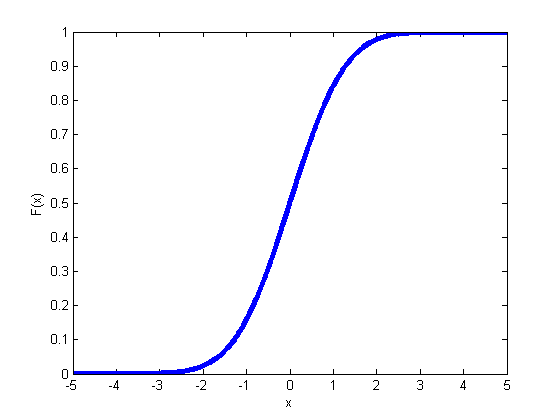
\includegraphics[scale=0.5]{./Slike/cdf.png} 
	\caption{Кумулативна функција расподеле \\ за случајне променљиве непрекидног типа} 
	\label{fig:slika13}
\end{figure}



\subsubsection{Вишедимензионалне случајне прменљиве}

Случајна променљива представља пресликавање скупа догађаја у реалне бројеве. Дакле, излази експеримента се мапирају у једнодимензионалан простор реалних бројева. Међутим, постоје случајеви када је потребно излазе експеримента мапирати у вишедимензионалне реалне просторе. На пример, при истовременом бацању два новчића могућа су 4 исхода :
\begin{enumerate}
\item $s_1$: први новчић писмо - други новчић писмо
\item $s_2$: први новчић писмо - други новчић глава
\item $s_3$: први новчић глава - други новчић писмо
\item $s_4$: први новчић глава - други новчић глава
\end{enumerate}

Нека је са $X_1$ означена случајна променљива која узима вредност 1 ако се на првом новчићу појавила глава, односно 0 ако се појавило писмо и аналогно $X_2$ која на исти начин означава појаву главе на другом новчићу. Исход експеримента се сада може описати дводимензионалном променљивом $(X_1,X_2)$. Графички приказ ове дводимензионалне промељиве дат је на следећој слици :

\begin{figure}[H]
    \centering
\captionsetup{justification=centering}
   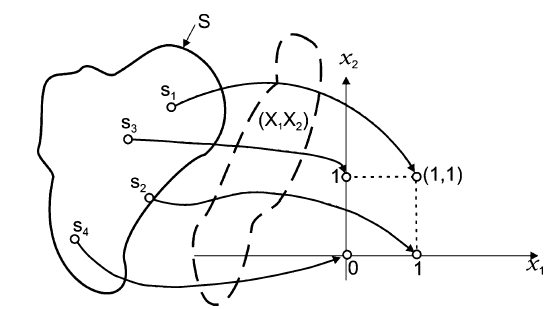
\includegraphics[scale=0.8]{./Slike/slika17.png} 
	\caption{Експеримент :  бацање два новчића. \\ Скуп $S$ представља скуп свих елементарних исхода ( $\Omega$)} 
	\label{fig:slika17}
\end{figure}





\begin{de}
Ако су $X : \Omega -> \mathbb{R} , Y : \Omega -> \mathbb{R}$ случајне променљиве, тада се \textbf{уређени пар} $(X,Y)$ натива \textbf{дводимензионална случајна променљива}. Уређеним паром   $(X,Y)$ се  сваком исходу  $\omega \in \Omega$ придружује уређени пар бројева $(X(\omega),Y(\omega))= (x,y) \in \mathbb{R} \times \mathbb{R} = \mathbb{R}^2$.
\end{de}

На следећој слици графички је представљена дводимензионална случајна применљива.



\begin{figure}[H]
    \centering
\captionsetup{justification=centering}
   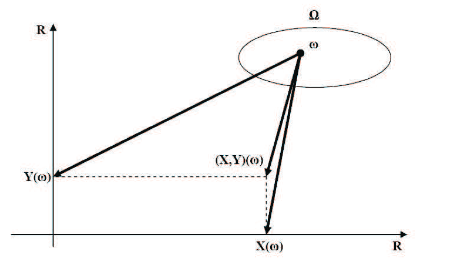
\includegraphics[scale=0.8]{./Slike/slika16.png} 
	\caption{Дводимензионална случајна променљива} 
	\label{fig:slika13}
\end{figure}

Овако уведен појам дводимензионалне случајне променљиве се може проширити и на више димензија и тада настају $n$-димензионалне случајне променљиве. Закључци изведени за дводимензионалне се такође односе и на вишедимензионалне случајне приоменљиве.

\textbf{Кумулативна функција расподеле} ( још се назива и \textit{заједничка расподела енг. joint distribution} дводимензионалне случајне променљиве, у ознаци $ F_{XY} : \mathbb{R}^2 -> [0,1] $ дефинише се као вероватноћа реализације догађаја $ \lbrace X \leq x , Y \leq y \rbrace $ односно :
$$
F_{X,Y}(x,y) = P \lbrace X \leq x, Y \leq y \rbrace \quad  - \infty < x,y < \infty
$$

Неке карактеристике функције расподеле дводимензионалне случајне променљиве :

\begin{enumerate}

\item  $ 0 \leq F_{X_1,X_2}(x_1,x_2) \leq 1 $
\item  $ F_{X_1,X_2}(-\infty,-\infty) =0 $
\item  $ F_{X_1,X_2}(-\infty,-\infty) =0 $  \\
$ F_{X_1,X_2}(-\infty,x_2) =0 $
$ F_{X_1,X_2}(x_1,-\infty) =0 $
\item  $ F_{X_1,X_2}(\infty,\infty) =1 $
\item  \begin{equation}
F_{X_1,X_2}(x_1,\infty) = F_{X_1}(x_1) 
\end{equation} 
\item 
\begin{equation}
F_{X_1,X_2}(\infty,x_2) = F_{X_2}(x_2) 
\end{equation} 

\end{enumerate}


Једнакостима (3.13) и (3.14) су дефинисане \textbf{маргиналне расподеле} случајних променљивих $X_1$ и $X_2$. Маргиналне расподеле су уствари расподеле једнодиментионалних случајних променљивих $X_1$ и $X_2$. На следећој слици је предсављена заједничка расподела две случајне приоменљиве заједно са њиховим маргиналним расподелама.

\begin{figure}[H]
    \centering
\captionsetup{justification=centering}
   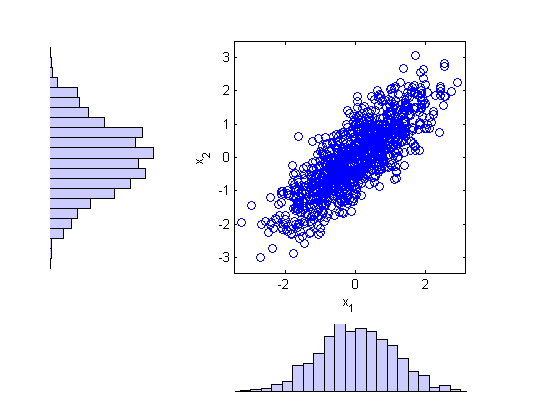
\includegraphics[scale=0.8]{./Slike/slika19.png} 
	\caption{Дводимензионална случајна променљива и маргиналне расподеле} 
	\label{fig:slika13}
\end{figure}


\textbf{Заједничка функција густине} (енг. joint density function) дводимензионалне случајне променљиве се дефинише као :

\begin{equation}
f_{X_1,X_2}(x_1,x_2) = \frac{d^2 F_{X_1,X_2}(x_1,x_2)}{dx_1dx_2}
\end{equation}

У случају једнодимензионалне случајне променљиве, површина испод графика функције густине на неком интервалу предстваљала је вероватноћу да случајна променљива узме вредност из тог интервала. У случају дводимензионалне случајне промељиве од интереса је пронаћи вероватноћу да она узме вредност из неке \textbf{области}. Та вероватноћа представља \textbf{запремину} тела ограниченог функцијом густине са горње стране и датом облашћу са доње стране.

\begin{figure}[H]
    \centering
\captionsetup{justification=centering}
   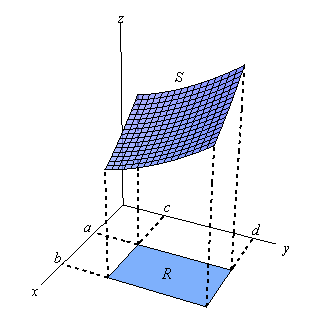
\includegraphics[scale=0.8]{./Slike/slika18.png} 
	\caption{Вероватноћа да дводемнзионална случајна промељива $(X,Y)$ узме вредности из области $R$} 
	\label{fig:slika18}
\end{figure}

 
Неке особине функције густине :

\begin{enumerate}
\item  $ \int \limits_{-\infty}^{\infty}\int \limits_{-\infty}^{\infty} f_{X_1,X_2}(x_1,x_2)dx_1dx_2 = 1$
\item  $F_{X_1,X_2}(x_1,x_2) =  \int \limits_{-\infty}^{x_1}\int \limits_{-\infty}^{x_2} f_{X_1,X_2}(x_1,x_2)dx_1dx_2$
\item  $F_{X_1}(x_1) =  \int \limits_{-\infty}^{x_1}\int \limits_{-\infty}^{\infty} f_{X_1,X_2}(x_1,x_2)dx_1dx_2$ \\
$F_{X_2}(x_2) =  \int \limits_{-\infty}^{x_2}\int \limits_{-\infty}^{\infty} f_{X_1,X_2}(x_1,x_2)dx_1dx_2$ 
\item $f_{X_1}(x_1) =  \int \limits_{-\infty}^{\infty} f_{X_1,X_2}(x_1,x_2)dx_2$ \\
$f_{X_2}(x_2) =  \int \limits_{-\infty}^{\infty} f_{X_1,X_2}(x_1,x_2)dx_1$ 
\item $P \lbrace x_{11} < X_1 \leq x_{12}, x_{21}<X_2 \leq x_{22} \rbrace =  \int \limits_{x_{21}}^{x_{22}}\int \limits_{x_{11}}^{x_{12}} f_{X_1,X_2}(x_1,x_2)dx_1dx_2 $
	
\end{enumerate}


\textbf{Функција условне расподеле и густине}


У неким специфичним случајевима је потребно пронаћи расподелу једне случајне променљиве знајући вредност друге случајне променљиве. Таква расподела назива се \textbf{условном расподелом} и обележава се са $F_{X_1}(x_1 \mid X_2 = x_2)$ . Аналогно, може се дефинисати и проблем налажења функције густине једне случајне променљиве знајући вредност друге случајне променљиве и таква функција густине  се означава са $f_{X_1}(x_1 \mid X_2 = x_2 )$. Према \cite{verov4} условна расподела односно густина се рачуна по следећем обрасцу ( детаљно извођење се може наћи у \cite{verov4})

$$  F_{X_1}(x_1 \mid X_2 = x_2) = \frac{\int \limits_{-\infty}^{x_1} f_{X_1,X_2}(x_1,x_2)dx_1}{f_{X_2}(x_2)} $$
односно :
$$  f_{X_1}(x_1 \mid X_2 = x_2) = \frac{f_{X_1,X_2}(x_1,x_2)}{f_{X_2}(x_2)} $$




\section{Важније расподеле}
\subsection{Бинонма и полиномна(енг. multivariate ) расподела}

\textbf{Бинонма расподела}

Нека ја А догађај неког екесперимента Е који се реализује са вероватноћом  $P(A) = p$. Тада је вероватноћа супротног догађаја $P(\overline{А}) = 1-p = q$. 
Резултат експеримента који је до интереса је остваривање или неостваривање догађаја А. Дакле, може се сматрати да је скуп свих елементарних исхода $\Omega = \lbrace A, \overline{A} \rbrace$. Нека се експеримент понавља \textbf{независно} и у неизмењеним условима $n$ пута. На тај начин је формиран \textbf{сложени експеримент} чији  скуп елементарних исхода садржи све могуће $n$-торке састављене од $А$ и $\overline{A}$ и има их укупно $2^n$. Нека је, даље, на том скупу елементарних исхода дефинисана случајна променљива $X_n$ као  број остваривања догађаја А у $n$ понављања експеримента Е. Вероватоћа да ова случајна променљива узме конкретну вредност $k$ је :
$$
p_k = P \lbrace X_n = k \rbrace ={ n \choose k} p^kq^{n-k}
$$

Вероватноће $P \lbrace X_n = k \rbrace ,(k=0,1,..,n)$ дефинишу\textbf{ биномну расподелу}, у ознаци $\mathbb{B}(n,p)$ . Ова расподела је дискретног типа а њена функција расподеле(кумулативна) се може изразити као :
$$
F(x)=\left\lbrace
\begin{array}{cc}
0 & , x \leq 0 \\
\sum_{k=0}^{r} {n \choose k} p^kq^{n-k} & 0 < r < n \\
1 & x > n
\end{array}
\right.
$$

Закон расподеле вероватноћа случајне променљиве биномне расподеле приказан је на следећој слици :


\begin{figure}[H]
    \centering
\captionsetup{justification=centering}
   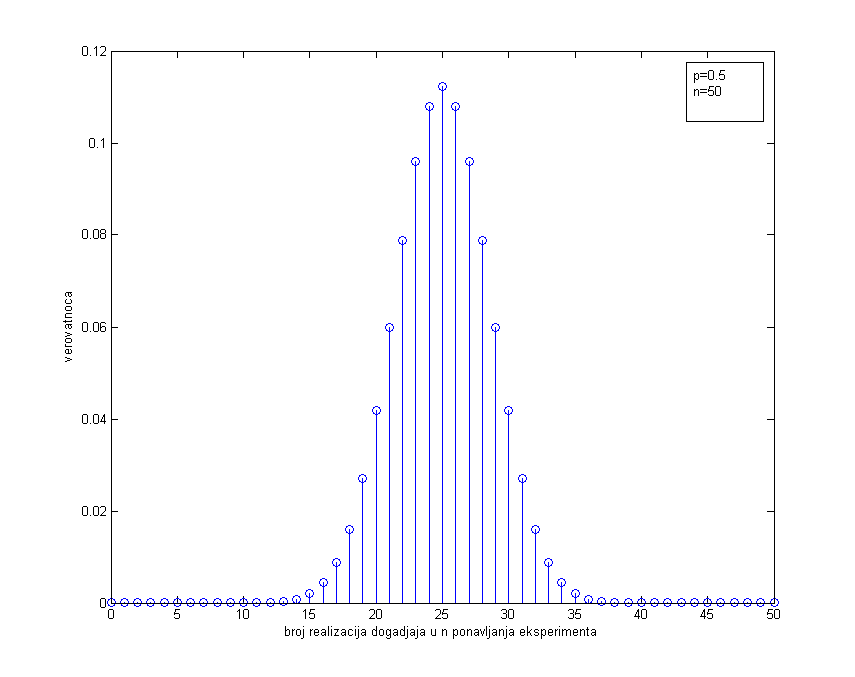
\includegraphics[scale=0.5]{./Slike/slika28.png} 
	\caption{Биномна расподела - закон расподеле} 
	\label{fig:slika20}
\end{figure}

\textbf{Полиномна (енг. multivariate) расподела}

Изводи се серија од $n$ независних експеримената при чему резултат експеримента може бити један од \textbf{коначно много} догађаја : $ A_1,A_2,..,A_k, \sum_{i=1}^k A_i = \Omega, P(A_i)=p_i (i=1,2,..k)$. 
Ако се дефинише $k$-диментионална случајна применљива $(S_n^{(1)},...,S_n^{(k)})$, где $S_n^{(i)}$ предстваља број релаизација случајног догађаја $A_i$ у  $n$ независних експеримената, тада важи :

$$
P(S_n^{(1)}=r_1,..,S_n^{(k)}=r_k) = \frac{n!}{r_1!..r_k!}p_1^{r_1}...p_k^{r_k} $$
$$
r_1,..r_k \in \lbrace 0,1,..,n \rbrace \quad
r_1+..+r_k = n
$$

Ако се са $S = (S_n^{(1)},...,S_n^{(k)})$ означи $k$-диментионална случајна применљива која има полиномијалну расподелу тада се то записује као :
$$
S \sim Mult(n,p)
$$
где је $p = (p_1,p_2,..,p_k)$
Пример полиномне расподеле при чему резулатат експеримента може бити један од \textbf{три} догађаја, дат је на следећој слици :


\begin{figure}[H]
    \centering
\captionsetup{justification=centering}
   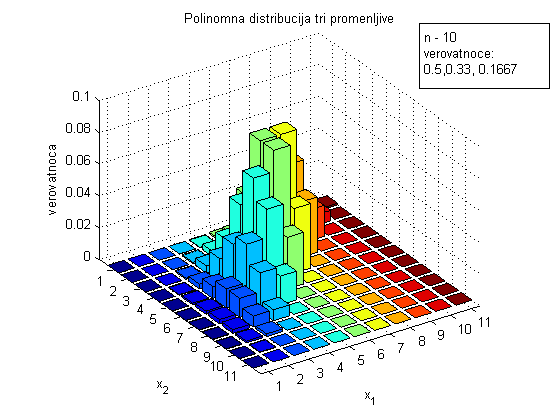
\includegraphics[scale=0.8]{./Slike/slika29.png} 
	\caption{Биномна расподела - закон расподеле} 
	\label{fig:slika20}
\end{figure}


%\subsection{Matrica kovarijanse,disperzija, aritmeticka sredina, multivariate normal distribution, conugate prior}


\subsection{Дирихлеова расподела}

Дирихлеова расподела представља фамилију расподела \textbf{за параметре} $p$  полиномијалне расподеле. Задаје се са :

$$
Dir(p;\alpha) = \frac{1}{B(\alpha)}\prod_{k=1}^{K}p_k^{\alpha_k -1}
$$

при чему је $\alpha$ параметар расподеле а $B$ означава мултиномијалну \textit{бета функцију}. 
Мултиномијалну бета функција се изражава преко гама фунцкије на следећи начин

$$B(\alpha) = \frac{\prod_{i=1}^{|\alpha|}\Gamma(\alpha_i)}{\Gamma(\sum_{i=1}^{|\alpha|}\alpha_i)}$$


На слећој слици је графички предстваљена Дирихлеова расподела за три променљиве :

\begin{itemize}
\item $\alpha = (1,2,3)$
\begin{figure}[H]
\minipage{0.45\textwidth}
  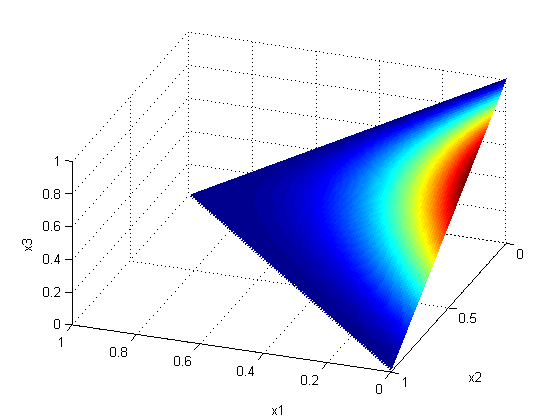
\includegraphics[scale=0.4]{./Slike/slika31.png} 
  \caption{Дирихлеова расподела - интензивнија боја предтсваља већу вероватноћу}\label{fig:slika25}
\endminipage\hfill
\minipage{0.45\textwidth}
  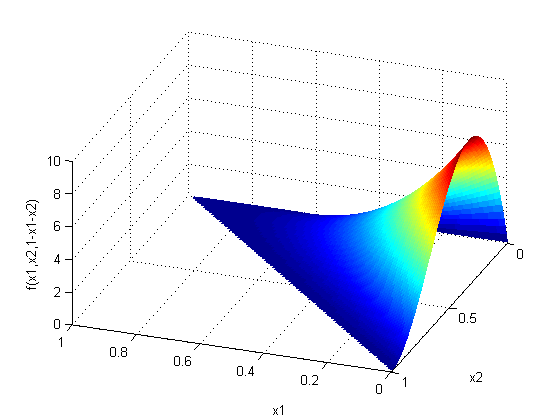
\includegraphics[scale=0.4]{./Slike/slika32.png} 
  \caption{Дирихлеова расподела у три димензије}\label{fig:slika26}
\endminipage\hfill

\end{figure}
\item $\alpha = (1,1,1)$
\begin{figure}[H]
\minipage{0.45\textwidth}
  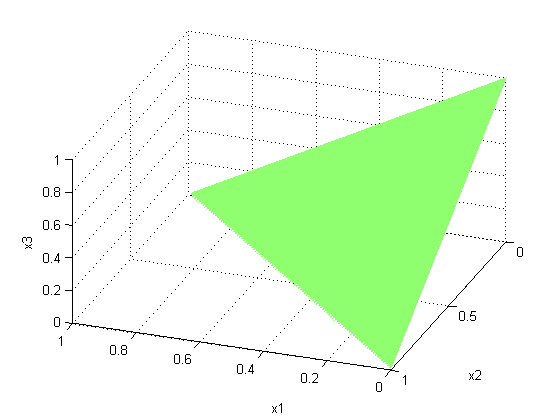
\includegraphics[scale=0.4]{./Slike/slika33.png} 
  \caption{Дирихлеова расподела - интензивнија боја предтсваља већу вероватноћу}\label{fig:slika25}
\endminipage\hfill
\minipage{0.45\textwidth}
  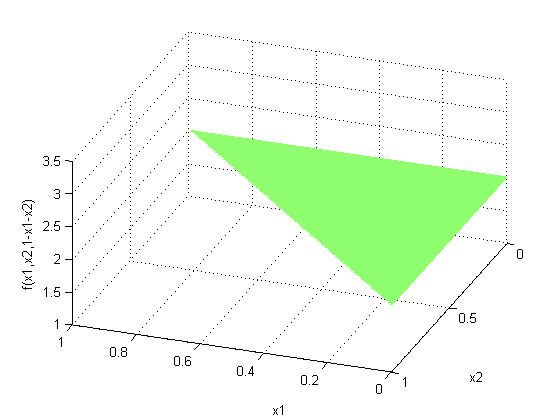
\includegraphics[scale=0.4]{./Slike/slika34.png} 
  \caption{Дирихлеова расподела у три димензије}\label{fig:slika26}
\endminipage\hfill

\end{figure}

\item $\alpha = (3,3,5)$
\begin{figure}[H]
\minipage{0.45\textwidth}
  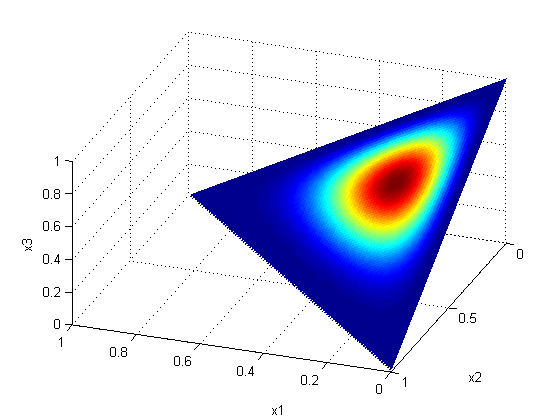
\includegraphics[scale=0.4]{./Slike/slika35.png} 
  \caption{Дирихлеова расподела - интензивнија боја предтсваља већу вероватноћу}\label{fig:slika25}
\endminipage\hfill
\minipage{0.45\textwidth}
  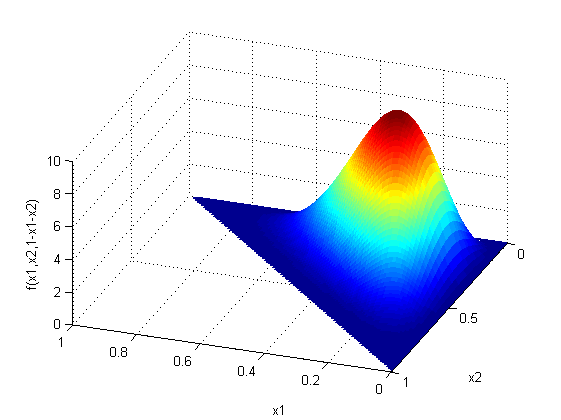
\includegraphics[scale=0.4]{./Slike/slika36.png} 
  \caption{Дирихлеова расподела у три димензије}\label{fig:slika26}
\endminipage\hfill

\end{figure}
\end{itemize}

\section{Гибсово узорковање}
\subsection{Марковљеви ланци}
Марковљевим ланцима моделује се математички сиситем стања и прелаза међу тим стањима. 
\begin{de}
Случајан (стохастички) процес представља математички модел процеса чија је еволуција описана законима вероватноће. \\
Марковљеви процеси су они случајни процеси чије будуће стање зависи само од тренутног стања. Оваква особина још се назива и \textit{одсуство памћења} \\
Марковљеви ланци представљају посебну врсту Марковљевих процеса где се процес може налазити само у коначном броју стања.
\end{de}

Пример Марковљевог ланца дат је на следећој слици :


\begin{figure}[H]
    \centering
\captionsetup{justification=centering}
   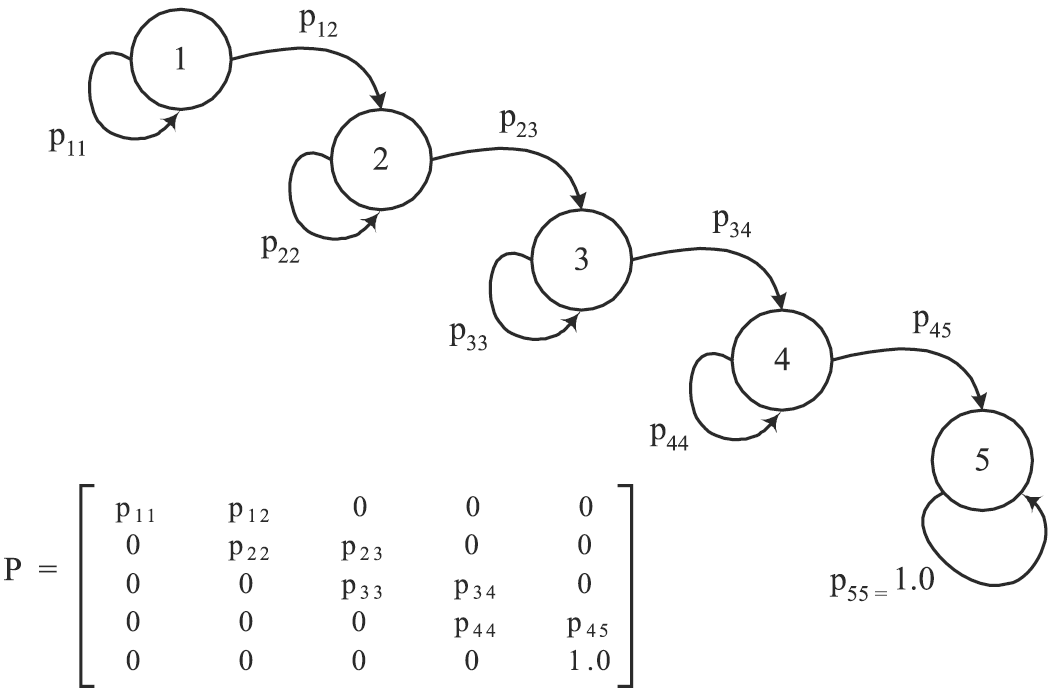
\includegraphics[scale=0.8]{./Slike/slika20.png} 
	\caption{Марковљев ланац - графички пример и матрица транзиције} 
	\label{fig:slika20}
\end{figure}

Систем се састоји од 5 стања. У сваком стању, са одређеним вероватноћама систем може да пређе у неко од следећих стања - конкретно да остане у тренутном стању или да пређе у једно стање ниже. Вероватноћа преласка у следеће стање зависи само од тренутног стања. Марковљеви ланци се често представљају \textbf{матрицама транзиције} при чему $i$-та врста у матрици садржи вероватноће преласка у свако од стање система када се систем налази у стању  $i$. Сума свих вероватноћа у свакој врсти је 1 ( систем сигурно мора да се нађе у неком стању, дакле вероватноћа да систем пређе у неко стање, могуће исто, је 1 ). Свака врста представља условни закон расподеле вероватноћа да систем пређе у било које стање у односу на тренутно стање ( $i$-та врста - $i$-то стање ).
Сака колона представља маргиналну расподелу вероватноћа да се систем нађе у одређеном стању ( $i$-та колона - $i$-то стање ). 


Систем се у једном тренутку може налазити у само једном стању. Нека се стање система карактерише случајном премнљивом  $X_n$ која у тренутку $n$  има расподелу $\overrightarrow{s}$ и нека је укупан број стања система $M$. Расподела $\overrightarrow{s}$ је у ствари закон расподеле (енг. PMF) јер се ради о случајној променљивој дискретног типа - систем може бити само у једном од  $M$ могућих стања, и конкретно може се посматрати као вектор врсте, димензија $1\times M$ где се на $i$ - том месту налази вероватноћа да се систем у тренутку   $n$ нађе у стању $i$.
 
У следећем временском тренутку,  $n+1$, систем се може наћи у било ком од $M$ стања са различитим вероватноћама. Вероватноћа да ће се систем у тренутку  $n+1$  наћи у стању $ј$ означава се са $P(X_{n+1} = j)$. Пошто ова вероватноћа зависи од стања у претходном тренутку, може се изразити на следећи начин ( према формули тоталне вероватноће )
$$
P(X_{n+1} = j) = \sum_{i}^{M} P(X_{n+1}=j \mid X{n}=i)P(X{n}=i) = *  $$
$P(X_{n+1}=j \mid X{n}=i)$ = вероватноћа преласка система из стања i у стање j  -> $p_{i,j} $ \\
$P(X{n}=i)$ = вероватноћа да се систем у тренутку n нађе у стању i -> $s_i$
$$
* = \sum_{i}^{M} p_{i,j}s_{i}
$$
Дакле, верованоћа да систем у  $n+1$-ом тренутку буде у стању $ј$ једнака је суми производа вероватноћа да се систем у $n$ -том тренутку нађе у било ком стању и вероватноћа одговарајућих прелаза. 

Ова сума представља $j$-ту колону у матрици ( димензија $1 \times M$ ) која се добије при множењу вектора  $\overrightarrow{s}$ и матрице транзиције $P$.

Према свему наведеном следи да је закон расподеле случајне променљиве $X_{n+1}$ ( расподела вероватноћа да се систем у  $n+1$-ом тренутку налази у сваком од стања ) једнак $\overrightarrow{s} \times P$.

Аналогно, у тренутку  $n+2$, случајна променљива   $X_{n+2}$ има расподелу  $\overrightarrow{s} \times P^2$, у тренутку $n+3$, случајна променљива   $X_{n+3}$ има расподелу  $\overrightarrow{s} \times P^3$ итд.

\begin{de}
Расподела  $\overrightarrow{s}$ за коју важи : 
$$
\overrightarrow{s} \times P = \overrightarrow{s}
$$
назива се \textbf{стационарна} или \textbf{равнотежна} расподела. 
\end{de}
$\overrightarrow{s} \times P $ представља "један корак у будуђност", тј. расподелу вероватноћа да систем нађе у сваком од стања у следећем временском тренутку. Уколико расподела остаје иста, односно, вероватноће се не мењају са временом, тада се та расподела назива стационарном. Под одређеним условима везаним Марковљеве ланце, доказује се да Марковљев ланац \textbf{увек} конвергира ка својој стационарној расподели без обзира на полазно стање. Више о конвергенцији Марковљевих ланаца може се наћи у \cite{verov6}. Дакле, полазне стање се може изабрати потпуно случајно а затим, уколико се дозвволи да "протекне" довољно времена, закон расподеле вероватноће да се систем нађе у свим стањима система ће конвергирати ка стационарној расподели тог ланца.


\begin{de}
MCMC ( енг. Markov Chain Monte Carlo ) методе представљају класу алгоритама који се користе за синтетичко генерисање узорака случајних променљивих из одговрајућих расподела. Овим методама се креирају Мерковљеви ланаци који као равнотежну расподелу имају расподелу из које се узимају узорци. Једна од MCMC метода је и Гибсово узорковање ( енг. Gibbs sampling )
\end{de}


\textbf{Гибсово узорковање} 

Нека је дата заједничка расподела (енг. joint distribution) $p(\textbf{z})= p(z_1,z_2,..,z_M)$ из које је потрбено одабрати неку вредност (енг. sample ) и нека је познато  почетно стање Марковљевог ланца који је потребно генерисати. Сваки корак Гибсовог узорковања почиње заменом  вредности једне променљиве  $z_1,z_2,..,z_M$ вредношћу која се добија из \textbf{условне расподеле} те променљиве у односу на све остале.  Дакле, $z_i$ се мења вредношћу која се узима из расподеле $p(z_i \mid z_{-i})$, где је са $z_i$ означена $i$-та координата вектора $z$  а са   $z_{-i}$ сви $z_1,z_2,..,z_M$ без $z_i$. Ова процедура се наставља за све променљиве по неком одређеном редоследу. При довољном броју итерација, врсности вектора $z$ ће конвергирати ка $p(z)$.

На пример, нека је дата расподела три случајне променљиве $p(z_1,z_2,z_3)$ и нека су вредности у тренутку $t : z_1^{t},z_2^{t},z_3^{t}$. Нека се замена вредности променљивих врши у односу на индекс, од најмањег ка највећем. Вредност $z_1^{t}$ се мења новом вредношћу  $z_1^{t+1}$ која се узима ( узрокује ) из расподеле 
$$
p(z_1|z_2^{t},z_3^{t}).
$$
Сада се вредност $z_2^{t}$ мења са вредношћу  $z_2^{t+1}$ која се узима из расподеле 

$$
p(z_2|z_1^{t+1},z_3^{t}).
$$

Дакле, одмах се користи нова вредност променљиве $z_1$. Коначно, за промену вредности $z_2^{t}$ користи се вредност $z_3^{t+1}$ која се добија из расподеле :

$$
p(z32|z_1^{t+1},z_2^{t+1}).
$$

Овим је завршена \textbf{једна итерација} Гинбсовог узорковања. Исти процес се наставља кроз низ итерација све до одређеног броја или до неког другог услова заустављања.

Описана процедура се може уопштити и на више од три променљиве и може се представити следећим псеудокодом:

\begin{figure}[H]
    \centering
\captionsetup{justification=centering}
   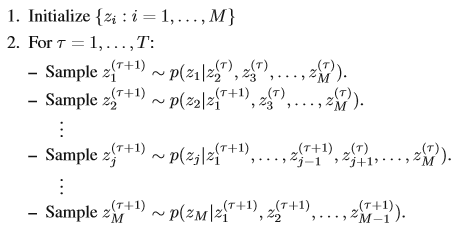
\includegraphics[scale=0.8]{./Slike/slika21.png} 
	\caption{Псеудокод Гибсовог узорковања, преузето са \cite{verov7}} 
	\label{fig:slika20}
\end{figure}


Гибсово узорковање подразумева да су унапред познате  \textbf{условне расподеле} свих променљивих и да је могуће узорковање из њих.

\textit{Пример :} Нека је потребно узорковати вредности из дводимензионалне нормалне расподеле $ \mathcal{N}(\mu, \Sigma )$ Гибсовим узорковањем при чему је 

$$\mu = [\mu_1,\mu_2] = [0,0]$$
$$\Sigma = \left[
\begin{array}{cc}
1 & \rho_{12} \\
\rho_{21} & 1
\end{array}
\right] =  \left[
\begin{array}{cc}
1 & 0.8 \\
0.8 & 1
\end{array}
\right]$$

Графички приказ овакве дводимензионалне нормалне расподеле дат је на следећој слици ( тродимензионално и пројектовано на две димензије ):

\begin{figure}[H]
\minipage{0.45\textwidth}
  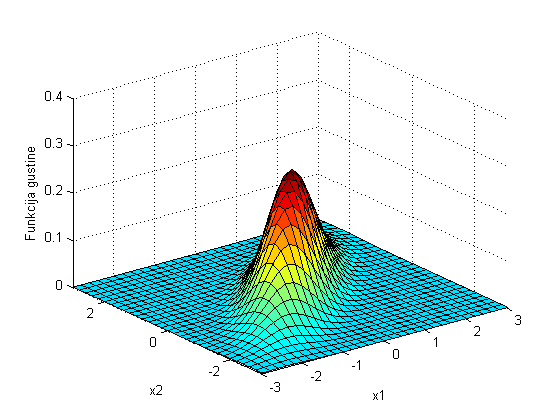
\includegraphics[scale=0.5]{./Slike/slika25.png} 
  \caption{Тродимензионални приказ дводимензионалне нормалне расподеле}\label{fig:slika25}
\endminipage\hfill
\minipage{0.45\textwidth}
  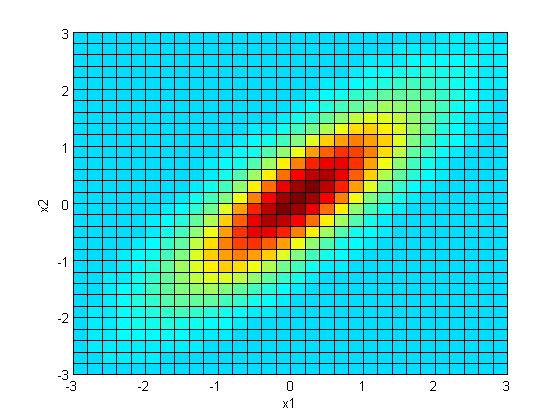
\includegraphics[scale=0.5]{./Slike/slika26.png} 
  \caption{Дводимензионлни приказ дводимензионалне нормалне расподеле}\label{fig:slika26}
\endminipage\hfill

\end{figure}

Основна претпоставка Гибсовог узорковања је да су познате условне расподеле свих променљивих и да је из њих могуће узорковати. Према \cite{verov7} и \cite{verov8}, за условне расподеле дводимензионалне заједничке расподел важи :
$$
p(x_1 \mid x_2^{(t-1)}) = \mathcal{N}(\mu_1 + \rho_{21}(x_2^{(t-1)} - \mu_2),\sqrt{1-\rho_{21}^2})
$$
и
$$
p(x_2 \mid x_2^{(t)}) = \mathcal{N}(\mu_2 + \rho_{12}(x_2^{(t)} - \mu_2),\sqrt{1-\rho_{12}^2})
$$
Дакле, обе условне расподеле представљају једнодимензионалну нормалну расподелу са одговарајућим параметрима.
Почетне вредности променљивих се бирају случајно зато што нису од важности. Марковљев ланац ће свакако конвергирати ка дводимензионалној нормалној расподели са неведеним параметрима после одређеног броја итерација. У зависности од полазног стања, тај број итерација ће бити мањи или већи.

На следећем сликама су предстваљене добијене расподеле Гибсовим узорковањем за различите почетне вредности :


\begin{figure}[H]
\minipage{0.32\textwidth}
  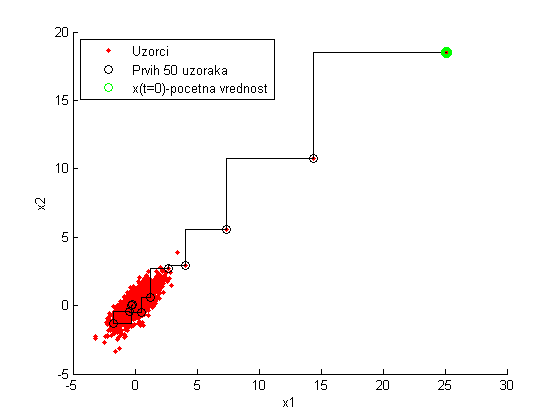
\includegraphics[scale=0.4]{./Slike/slika22.png} 
  \caption{Почетна тачка (25.1284,18.5165)}\label{fig:slika22}
\endminipage\hfill
\minipage{0.32\textwidth}
  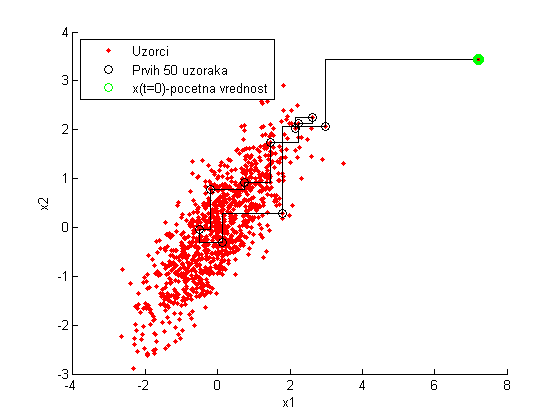
\includegraphics[scale=0.4]{./Slike/slika23.png} 
  \caption{Почетна тачка (7.2162, 3.4380)}\label{fig:slika23}
\endminipage\hfill
\minipage{0.32\textwidth}%
   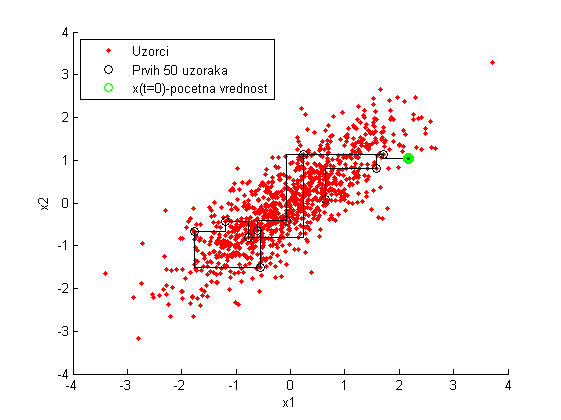
\includegraphics[scale=0.4]{./Slike/slika24.png} 
  \caption{Почетна тачка ( 2.1649, 1.0314)}\label{fig:slika24}
\endminipage
\end{figure}

Са слика је очигледно да се првих неколико узорака може занемарити (\ref{fig:slika22} може се занемарити првих 7-8 узорака).

Важно је приметити да се узимање узорака увек креће по "степенастом" обрасцу. Дакле, две суседне тачке имају исту једну координату ($x$ или $y$). То је зато што  Гибсово узорковање у једном тренутку мења \textbf{само једну} променљиву у односу на одговарајућу вредност друге.

Конвергенција алгоритма Гибсовог узорковања ка стационарној расподели Марковљевог ланца је теоретски загарантована, али је у пракси јако тешко одредити број итерација након којих ланац почиње да конвергира. Један од начина процене конвергенције је и рачунање \textit{log-likelihood} -а

\section{Како ради ТМ алгоритам}

Раније је неформално описан  LDA генеративни процес. Основна претпоставка је да се сваки документ у одређеној пропорцији говори о свакој теми ( има одређену расподелу над темама) као и да свакој теми све речи из корпуса припадају са различитим вероватноћама ( расподела над речима).  Генеративни процес се , према \cite{verov9}, може описати следећим псеудокодом :

\begin{figure}[H]
  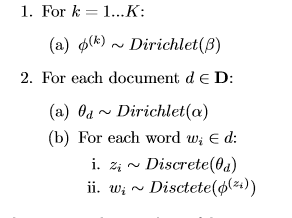
\includegraphics[scale=0.8]{./Slike/slika27.png} 
  \caption{Генеративни процес LDA-а }\label{fig:slika27}
\end{figure}

при чему је :
$K$ - укупан број тема у колекцији
$\phi_{(k)}$ -  расподела над свим речима из колекције и представља расподелу над речима у $k$-тој теми
$\theta_d$ - расподела над темама у документу $d$.
$z_i$ - тема којој припада реч $w_i$.
$\alpha,\beta$ - \textbf{хиперпараметри} тј. параметри симетричних Дирехлеових расподела.

Описани генеративни процес резултује формирањем следеће заједничке расподеле :

\begin{equation}
p(w,z,\theta,\phi \mid \alpha,\beta) = p(\phi \mid \beta)p(\theta \mid \alpha)p(z \mid \theta)p(w \mid \phi_z)
\end{equation}
Непозанте променљиве које је потребно "открити" су $z,\theta$ и $\phi$ на основу (једино) познатих  \textbf{речи} и њиховог присуства у сваком од докумената. Дакле, потребно је пронаћи расподеле наведених променљивих \textbf{под условом} да су познате речи и њихова распоређеност по документима тј. открити њихове постериорне расподеле.
Основни проблем ТМ је  \textbf{постериорно закључивање} (енг. posterior inference) односно отривање постериориних расподела латентних случајних променљивих на основу задатог скупа докумената и речи што представља решавање следеће једначине :

\begin{equation}
p(\theta,\phi,z \mid w,\alpha,\beta) =\frac{p(\theta,\phi,z,w,\mid \alpha,\beta)}{p(w \mid \alpha,\beta)}
\end{equation}

Према  \cite{verov9}, рачунање имениоца овог разломка је готово немогуће па се стога прибегава апроксимативним методама каква је и Гибсово узорковање.

Да би се применило Гибсово узорковање, потребно је познавати  условне расподеле свих променљивих из чије се заједничке расподеле узоркује. Међутим, показује се да је довољно пронаћи само $z$ јер се остале две променљиве могу преко ње израчунати и то (према \cite{verov9}):

$$
\theta_{d,z} = \frac{n(d,z)+\alpha}{\sum_{|Z|}n(d,z)+\alpha}
$$
$$
\phi_{z,w} = \frac{n(z,w)+\beta}{\sum_{|W|}n(z,w)+\beta}
$$
 
Овако примењен алгоритам Гибсовог узорковања назива се још и енг. Collapsed Gibbs Sampling. Дакле, циљ је пронаћи за сваку реч, вероватноћу да припадне свакој од тема, под условом да су познате теме којима припадају остале речи у том тренутку. Формалније, ово се може записати $ p(z_i \mid z_{-i},\alpha,\beta,w)$ где $ z_{-i}$ предстваља доделу тема свим речима сем $i$-те. 

Априорне расподеле коришћене у ТМ су Дирихлеове.Важна особина Дирихлеове расподеле је да је она \textbf{конјугована} са мултиномијалном расподелом. 
Дирихлеова расподела је расподела над параметрима мултиномијалне расподеле. Нека је на почетку претпостављено да параметри мултиномијалне расподеле припадају некој Дирихелеовој расподели - $\mathbf{p} \sim Dir(\mathbf{p,\alpha})$. Нека је $\mathbf{x}$ узорак генерисан из мултиномијалне расподеле $Mult(\mathbf{x;p})$. Тада важи да је постериорна расподела $\mathbf{p}$ ( дакле, расподела под условом да је познат узорак  $\mathbf{x}$ ) такође \textbf{Дирихлеова расподела} са параметром $\mathbf{x+\alpha}$ тј.:
\begin{equation}
p(\mathbf{p\mid x,\alpha}) = Dir(\mathbf{p;x+\alpha}) = \frac{1}{B(\mathbf{x+\alpha}})\prod_{i=1}^{|\mathbf{\alpha}|} p_i^{x_i+\alpha_i-1}
\end{equation}

Како (3.18) представља \textbf{расподелу} то важи да је :

\begin{equation}
1 = \int \frac{1}{B(\mathbf{x+\alpha}})\prod_{i=1}^{|\mathbf{\alpha}|} p_i^{x_i+\alpha_i-1} = \frac{1}{B(\mathbf{x+\alpha}})\int \prod_{i=1}^{|\mathbf{\alpha}|} p_i^{x_i+\alpha_i-1}
\end{equation}
Одакле следи да је :

\begin{equation}
\int \prod_{i=1}^{|\mathbf{\alpha}|} p_i^{x_i+\alpha_i-1} = B(\mathbf{x+\alpha})
\end{equation}

Ова једнакост је важна за даљи опис рада ТМ алгоритма.

Према формули условне расподеле, важи :


\begin{equation}
p(z_i \mid z_{-i},\alpha,\beta,w) = \frac{p(z_i,z_{-i},w \mid \alpha,\beta)}{z_{-i},w \mid \alpha,\beta)} \propto p(z_i,z_{-i},w \mid \alpha,\beta) = p(z,w \mid \alpha,\beta)
\end{equation}

$p(z,w \mid \alpha,\beta)$ се може посматрати као "маргиналан расподела" две променљиве  заједничке расподеле (3.16)  па важи :

\begin{equation}
p(z,w \mid \alpha,\beta) = \iint p(z,w,\theta,\phi \mid \alpha,\beta)d\theta d\phi = \iint p(\phi \mid \beta)p(\theta \mid \alpha)p(z \mid \theta)p(w \mid \phi_z) d\theta d\phi 
\end{equation}

Груписањем по заједночкој зависној променљивој, претхонда једначина се може написати :

\begin{equation}
p(z,w \mid \alpha,\beta) = \int p(z \mid \theta)p(\theta \mid \alpha)d\theta \int p(w \mid \phi_z)p(\phi \mid \beta)d\phi
\end{equation}

Оба интерграла представљају комбинацију узорка из мултиномијалне расподеле и априорне Дирихлеове расподеле. Како је Дирихлеова расподела конјугована (conjugate prior) са мултиномијалном, у подинтегралном изразу се налази "множење" две Дирихлеове расподеле са одговарјућим параметрима.

Дакле :
Пошто  $p(z \mid \theta)$ има мултиномијалну дистрибуцију, важи:
\begin{equation}
p(z \mid \theta) = \prod_{i=1}^D \prod_{k=1}^K \theta_{d,k}^{\Omega_{d,k}}
\end{equation}
, где је $\Omega_{d,k}$ број који означава колико пута је тема $k$ додељена у документу $d$ - број речи који у документу $d$ припадају теми $k$.

Члан $p(\theta \mid \alpha)$ је из основне Дирихлеове расподеле па важи :

\begin{equation}
	p(\theta \mid \alpha)  {(1) \atop = }\prod_{i=1}^D p(\mathbf{\overline{q_d}} \mid \alpha) {(2) \atop = }
	 \prod_{d-1}^D \frac{1}{B(\alpha)}\prod_{k=1}^K q_{d,k}^{\alpha_k -1}
\end{equation}



где је $\mathbf{\overline{q_d}}$ расподела вероватноћа тема у документу $d$. Расподеле вероватноћа тема по документима су независне, па је зато могуће написати (1).Расподела тема по документу се узима из Дирихлеове расподеле па је зато могуће написати (2).

Према томе, први интеграл једнакости (3.23) се записује као :


\begin{equation}
	 \int p(z \mid \theta)p(\theta \mid \alpha)d\theta = \int \prod_{i=1}^D \prod_{k=1}^K \theta_{d,k}^{\Omega_{d,k}} \prod_{d-1}^D \frac{1}{B(\alpha)}\prod_{k=1}^K q_{d,k}^{\alpha_k -1}d\theta_d {(1) \atop = } \prod_{i=1}^D \int \frac{1}{B(\alpha)}\prod_{k=1}^K q_{d,k}^{\Omega_{d,k} +\alpha_k -1}d\theta_d 
\end{equation}
Једнакост (1) следи из чињенице да су $\theta_d $ независне расподеле па се могу интегралити посебно - правило интеграције производа
Према релацији (3.20) претходна једнакост се може написати и као се :
\begin{equation}
 \int p(z \mid \theta)p(\theta \mid \alpha)d\theta = \prod_{i=1}^D \frac{B(\Omega_d+\mathbf{\alpha})}{B(\mathbf{\alpha})}
\end{equation}

где је са $\Omega$ означена матрица докумената и тема, $\Omega_{d,k}$ означава колико је пута тема $k$ додељена у документу $d$ а $\Omega_d$ је $d$-та врста те матрице. Елементи ове матрице могу се математички записати и овако :

\begin{equation}
\Omega_{d,k} = \sum_{i=1}^N I(d_i=d \wedge z_i=k)
\end{equation}

где је $N$ укупан број речи у корпусу(са понављањем).

Аналогно претходним извођењима, и други интеграл може да се упрости:

Члан $p(\phi \mid \beta)$ је из основе Дирхлеове расподеле па важи :

\begin{equation}
p(\phi \mid \beta) = \prod_{k=1}^K p(\phi_k \mid \beta) = \prod_{k=1}^K \frac{1}{B(\beta)}\prod_{v=1}^V \phi_{k,v}^{\beta_v-1}
\end{equation}

Члан $p(w\mid\phi_z)$ има мултиномијалну расподелу па важи :

\begin{equation}
p(w\mid\phi_z) = \prod_{i=1}^N p(\phi_{z_i,w_i}) = \prod_{k=1}^K\prod_{v=1}^V\phi_{k,v}^{\Psi_{k,v}}
\end{equation}

где је $\psi \quad K \times V$ матрица а $\psi_{k,v}$ броји колико тема $k$ била додељена речи $v$. Ова матрице може се још написати као :

\begin{equation}
\psi_{k,v} = \sum_{i=1}^N I(w_i=v \wedge z_i = k)
\end{equation} 

На основу (3.29) и (3.30) следи :
\begin{equation}
\int p(w \mid \phi_z)p(\phi \mid \beta)d\phi = \int \prod_{k=1}^K \frac{1}{B(\beta)}\prod_{v=1}^V\phi_{k,v}^{\psi_{k,v}+\beta_v -1}d\phi_k
\end{equation}

Аналогно извођењу (3.26) (3.27) следи :

\begin{equation}
\int \prod_{k=1}^K \frac{1}{B(\beta)}\prod_{v=1}^V\phi_{k,v}^{\psi_{k,v}+\beta_v -1}d\phi_k =\prod_{k=1}^K (\frac{1}{B(\beta)} \int \prod_{v=1}^V\phi_{k,v}^{\psi_{k,v}+\beta_v -1}d\phi_k) = \prod_{k=1}^K \frac{B(\psi_k +\beta)}{B(\beta)}
\end{equation}

Коришћењем једнакости (3.27) и (3.33), једнакост (3.23) се може записати као :

\begin{equation}
p(z,w \mid \alpha,\beta) = \prod_{i=1}^D \frac{B(\Omega_d+\mathbf{\alpha})}{B(\mathbf{\alpha})}\prod_{k=1}^K \frac{B(\psi_k +\beta)}{B(\beta)}
\end{equation}

На основу (3.34) може се извести правило по коме ће Гибсов алгоритам узорковања мењати доделе тема речима. Дакле :

\begin{equation}
p(z_i=k|Z^{-i},W,\alpha,\beta) = \frac{p(z_i=k,Z^{-i},W \mid \alpha,\beta}{p(Z^{-i},W \mid \alpha,\beta)} = \frac{p(Z,W \mid \alpha,\beta)}{p(Z^{-i},W \mid \alpha,\beta)}
\end{equation}

Именилац претходне једноакост се може написати преко условне вероватноће у следећем облику :

\begin{equation}
p(Z^{-i},W \mid \alpha,\beta) = p(Z^{-i}\mid \alpha\beta)p(W \mid Z^{-i},\alpha\beta ){(1) \atop = } 
\end{equation}

\begin{equation}
=p(Z^{-i})p(W^{-i} \mid Z^{-i})p(w_i) \propto  p(Z^{-i})p(W^{-i} \mid Z^{-i})  = p(Z^{-i},W^{-i})
\end{equation}
Једнакост (1) следи из чињенице да свако $z_i$ зависи само од $w_i$. Од ове једнакости параметри $\alpha, \beta$ су изостављени због прегледсноти, али се подразумевају.

Форма једнакости (3.37) иста је као (3.31) па се једнакост (3.35) записује као :

\begin{equation}
p(z_i=k|Z^{-i},W,\alpha,\beta) = \prod_{k=1}^K\frac{B(\psi_k + \beta}{B(\psi_k^{-i}+\beta}\prod_{d=1}^D\frac{B(\Omega_d + \alpha}{B(\Omega_d^{-i} + \alpha}
\end{equation}

Коришћењем особина бета фунцкије, претходна једнакост се своди на :

\begin{equation}
p(z_i=k|Z^{-i},w=v,W^{-i},\alpha,\beta) = \frac{\psi_{k,v}+\beta_{w_i}-1}{\left[ \sum_{v=1}^V \psi_{k,v}+\beta_v \right] -1}\left[\Omega_{d,k}+\alpha_k-1 \right]
\end{equation}

Детаљно извођење може се нађи код \cite{verov9} и \cite{verov10}.

\subsection{Имплементација - псеудокод}
\textbf{Овде ће доћи мој псеудокод, ово је само привремено}
%\begin{algorithm}
%\caption{LDA}
%\label{CHalgorithm}
%\textbf{Ulaz:} reci $w$ i dokumeta $d$ \\
%\textbf{Izlaz:} dodeljene teme recima u svakom  dokumentu -  $z$
%\textbf{begin} \\
%Slucajno inicijalizuj z - svakoj reci u korpusu dodeli neku temu
%\begin{algorithmic}[1]
% \Foreach{iteracija}
% \State \For{$i=0\rightarrow N-1$}
% \State rec $\leftarrow w[i]$
% \State tema $\leftarrow z[i]$
% \State $n_{$
%
%\end{algorithmic}
%\end{algorithm}
\begin{figure}[H]
  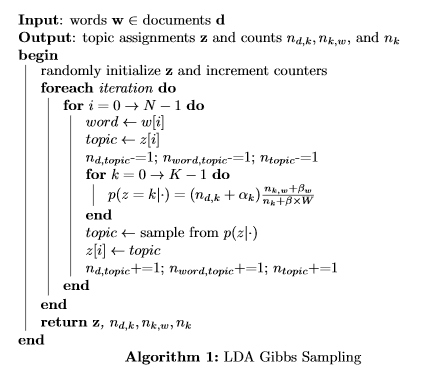
\includegraphics[scale=0.8]{./Slike/slika30.png} 
  \caption{Псеудокод - преузето са \cite{verov10} }\label{fig:slika27}
\end{figure}


%\chapter{Историја ТМ}
\chapter{Припрема подарака}

Подаци  кориштени за тестирање приликом израде овог рада су јавно доступни подаци са сајта \textbf{\textit{http://stackexchange.com/}} из три области  - инжињерство, фитнес и хемија. Подаци су на \textbf{енглеском језику}. 

Ове три области су намерно тако одабране како би се повећала разноврсност речи. Речи из сродних научних грана користе сличну или исту терминологују па опасност од бирања питања и одговора из  сродних научних дисциплина лежи у чињеници да ће диверзитет корпуса бити мали.

Из сваке области узето је по 200 питаља и одговора, што представља базу од укупно 600 питања и 600 одговора. Овакав скуп података је затим подељен на два дела - тренинг део (360 питања и одговора) и тест део (240 питања и одговора).

Након испитивања на овом скупу података, решење је тестирано и на подацима доступпним са сајта \textit{answers.yahoo.com}. На овај начин, "`дуплим"' тестирањем, обезбеђује се независност закључака од природе података.

Подаци добијени са означених сајтова нису погодни за директну обраду те их је потребно делимично \textbf{прерадити} тј. \textbf{предпроцесирати}. 

Надаље следи опис коришћених метода предпроцесирања. Приликом тестирања коришћене су различите комбинације ових метода и мерени су њихови утицаји на крајње решење.


	\section{Уклаљаље HTML ознака и неалфанумеричких карактера }
	
Подаци који су достуони преко сајта \textbf{\textit{http://stackexchange.com/}} дати су у форми HTML текстова. То значи да се кроз основни текст питања и одговора провлаче додатни низови карактера који представљају HTML ознаке (тагове). Ове ознаке добијају смисао приликом генерисања веб странице, односно приликом форматирања текста питања и одговора на веб страницама. Међутим, за обраду текста у овом раду, те ознаке не значе ништа и додатно могу уносити забуну. Због тога их је потребно, пре било какве даље обраде текста, склонити. Најједноставнији начин да се то уради је преко \textit{регуларних израза}, обзиром на изглед и формат HTML ознака.


Са друге стране, у тексту се поред слова и бројева (\textit{алфанумерички карактери}) обавезно појављују и специјални знаци (ознаке које нису ни слова ни бројеви - \textit{неалфанумерички карактери}, међукојима су најчешћи интерпукцијски знакови . Поред њих, у скорије време, уз сваки текст је готово обавана појава и група специјалних знакова као што су нпр. смајлићи ( структуре конструисане од специјалних знакова које се могу интерпретирати као расположење нпр. :) - срећа, :( - туга  итд. ). Са становишта алгоритма моделовања тема, сви они, исто као и HTML ознаке, немају значење и потребно их је уклонити. Такође, најједноставнији начин да се то уради је применом регуларних израза.

	\section{Конвертовање свих слова текста у "`мала слова"'  енг. lowercase }

Писање речи великим или малим словима, као и започињање речи малим или великим словом, углавном има граматички смисао. При томе, у већини случајева, реч написана почетним великим и иста реч написана почетним  малим словом, имају исто значење. У машинској обради података, свако слово има другачију бинарну репрезентацију. Стога, реч написана великим почетним словом и иста реч написана малим почетним словом или свим великим словима, \textbf{нису исте речи} обзиром на то да имају различиту репрезентациу. Како би се ово избегло, пре било какве даље обраде, врши се конвертовање или пребацивање свих слова текста у мала слова. На тај начин, све речи састављене од истих слова и у истом редоследу, представљају \textbf{исту} реч, без обзира на граматичко значење речи или њену позицију у тексту. Избор конвертовања у мала слова је једнако оправдан као и  конвертовање у велика слова. Дакле, исти резултат би се добио и конвертовањем свих слова у велика слова. Међутим, у пракси, је чешће прихваћено пребацивање у мала слова па је такав приступ усвојен и у овом раду.
Наравно, постоје бројни примери када писање речи великим или малим почетним словом битно мења значење речи. На пример, у српском језику, реч \textit{Мила}, написана великим почетним словом, означава име особе, именуцу, док реч \textit{мила}, написана малим почетним словом означава придев. Исто тако реч, \textit{Јела} односи се на име особе док се реч \textit{јела} односи на врсту зимзеленог дрвета. 
Међутим, оваквих речи има довољно мало да је ризик од мењања значења речи, са аспекта алгоритма моделовања тема, прихватљив.


\section{Издвајање атомских елемената докумената - токена, енг. tokenization}

Манипулација читавим документима са аспекта алгоритма моделовања тема, нема смисла. Основна јединица манипулације ове врста алгоритама је \textbf{реч}.  Према томе, потребно је документе рашчланити на поједниначне речи. Процес издвајања основних елемената манипулације, тј. елемената од интереса, назива се издвајање \textbf{токена} или \textbf{токенизација}. Обзиром да су овде атомски елементи \textbf{речи} и да су речи одвојене размаком, процес токенизације је најједноставније извршити преко регуларних израза. 
У пакету Mallet се већ налазе готове класе  

	\section{Избациваље често коришћених речи енг. stop words}
		
У свакодневном говору често се употребљавају личне заменице, прилози, везници итд. Без њих, говор би био неодређен и неповезан па самим и неразумљивив. Међутим, у машинској обради текстуланих података, поготово у алгоритмима моделовања тема, оваква врста информација није неопходна. Пре свега, такве  речи не носи суштинско теметско значење обзиром да нису уско повезана ни са једном конкретном области. На пример, везници ,као што су у српском језку: и, или, па, али, због, ради итд. се употребљавају при писању докумената из свих научних грана и стога се ни за једну од тих речи не може дефинисати област припадања. Обзиром да је циљ из групе докумената издвијити \textbf{теме}, овакве речи су сувишне. Штавише, уносе додатну забуну при закључивању и, обзиром да су бројене, могу представљати велико оптерећење приликом обраде.	
Подаци коришћени у при изради овог рада су на енглеском језику те ће се надаље говорити о оваквој врсти речи у енглеском језику. Међутим, узимањем уобзор специфичности конкретног језика, иста разматрања могу се применти и на друге језике.

Избацивање често коришћених речи, stop words-ова, може се реализовати на више начина. 

Поузданији, универзалнији али и рачински захтевнији начин је алгоритамско проналажење таквих речи. Обизором да немају тематско значење, оне се појављују у великом броју у свим документима и темама. Једноставним бројањем појављивања речи у скупу свих докумената могу се уочити групе речи које се са изузетно високим фреквенцијама јављају у \textbf{свим документима}. Такве речи се могу сматрати за често коришћене те се, из описаних разлога, избацују.  Поред једноставног бројања речи, постоје и друге методе "` мерења "' присуства речи у корпусу. Једна од њих је и релативна фреквенција која зависи од дужине докумената. Међутим, обзором да овај приступ није коришћен у раду, у ове методе се неће дубље улазити.

Други, мање поуздан и релативно рачиунски незахтеван приступ је коришћење \textbf{листе често коришћених речи} које постоје за сваки језик. Те листе су јавно доступне и могу се пронаћи на бројним веб сајтовима. Обзором да је циљ рада био истраживање примене алгоиртама моделовања тема у специфичном проблему, овај приступ је прихватљивији. Пре свега, релативно се лако имплеменртира обзором да у Mallet-у већ постоји класа за уклањање ових речи. Са друге стране, овај корак предпроцесирања се на овај начин претвара у тривијалан и оставља простор за истраживање самог алгоритма моделовања тема. 
Највећа опасности од овог приступа је елеминација речи које, иако сврстане међу често коришћене, у датом скупу докумената ипак имају значење. Исто тако, обзиром да је листа предефинисана, могуће је изоставити речи које у конкретном скупу представљају често коришћене речи.

За поузданије и детаљнија истраживања, предлаже се примена прве методе. 
 
 	
	
	\section{Додавање синонима}
У циљу бољег дифренцирања тематике питања и одговора, за сваку реч је додато по 5  синонима. За проналажење синонима је коришћена WordNet библиотека. Основни разлог додавања синонима у скуп била је претпоставка да ће се на тај начин боље диференцирати теме, повећати диверзитет корпуса а самим тим и олакшати препознавање тачног одговора. Међутим, резулатати су показали управо супротно. Разлог томе што синониме треба тражити \textbf{по смислу} речи а не само по лексичком облику речи. Такође, фразе, којих има доста у свакодневном говорном и писаном енглеском језику, значајно могу да утичу на смисао питања/одговора. Када се они рашчлане на појединачне речи, могуће је да се и смисао промени.

	\section{Склањање наставака речи - енг. stemming}
	
Овај сегмент предпроцесирања је изузетно завистан од језика на коме је текст писан. Циљ је препознати различите облике исте речи и свести је на заједничку основу, која \textbf{не мора} да буде коренска. У енглеском језику, различити облици речи граде се додавањем разних \textbf{наставака} као што су \textit{s,ing,es ...}. Дакле, склањањем наставака речи редукује се диверзитет корпуса али се истовремено речи које имају исто значење само различит облик настао услед контекста реченице - рода, времена, врсте речи итд, своде на исту реч. У конкретној примени, овако нешто је неопходно за прецизно раздвајање тема. 
За српски језик овако нешто не би било могуће имплементирати на једноставан начин обзором на промену речи по падежима, лицима ( за глаголе ), родовима, бројевима и гласовне промене које се при томе дешавају. У тренутку писања рада, никакво готово решења за српски језик није постојало. Уколико предмет истраживања неког будућег рада буде био српски језик, потребно је написати ппроцедуре којима се речи језика ослобађају наставака, следећи граматичка правила.

	
	\section{Свођење на коренску реч - енг. lemmitization}

Свођење речи на коренску реч је слична метода методи склањања наставака речи, такође уско повезена са језиком који се обрађује. Једна од  разлика је што се склањање наставака речи може применити на речи које мењају облик додавањем наставака док се свођење на коренски реч може применити на све речи. На пример,  реч енг. better - бољи, при склањању наставака би остала непромењена  или би се свела на реч енг. bett,  док при свођењу на коренску реч она постаје енг. good - добар.
Друга, битнија разлика, је што се уклањање наставака  примењује на речи не водећи рачуна о контексту, док се свођењем на коренску реч може специфицирати и контекст речи. На пример, реч енг. meeting - може имати више значења. Као именица она означава \textit{састанак} док као глагол означава презент партицип глагола \textit{to meet}, у смислу \textit{сретати се, }. Уклањањем наставака, реч енг. meeting  у контексту именице као и у контексту глагола биће сведена на реч енг. meet. Код свођења речи на коренску реч, спецификацијом врсте речи могуће је реч енг. meeting оставити непромењену.
Такође, свођењем на кореснку реч могуће је неправилне глаголе енглеској језика свести на основни облик, што склањањем наставака није било могуће. 
Са аспекта алгоритма моделовања тема, свођење на коренску реч је прихватњивија метода, пре свега због могућности препознавања различитог облика истих речи када се они не граде додавањем наставака.
Обзором на једноставност имеплементације и брзину рада, чешће се користи скалањање наставка од свођења на коренску реч. У конкретном раду, обе методе су независно тестиране и равноправно коришћене у циљу добијања бољих резултата.
	

\chapter{Решење проблема применом алгоритма моделовања тема}

%MILOS: Понови овде јасно шта је главни циљ рада. То смо поменули само у уводу, треба поново да се нагласи.
Проналажење правог одговора на постављено питање може бити изузетно сложен проблем, чак и за човека. Оно што је суштински важно за препознавање ваљаног одговора је разумевање \textbf{суштине} односно смисла питања. За разлику од машина, човек на основу знања уме да наслути тај смисао, а самим тим и да препозна адекватан одговор. Међутим, уколико би се пред човека ставило питање из области о којој он нема никаквог знања (не разуме значење термина), или је на језику који не разуме, врло је вероватно да би препознавање правог одговора било врло непоуздано. 
Са друге стране, немогуће је не запитати се шта заправо представља прави одговор на постављено питање. Данас је можда лакше него икада поставити питање и у кратком времену добити велики број одговора од различитих корисника. Учесници конверзације не морају нужно бити стручњаци из области која се тиче питања. Исто тако, велики број одговора, иако су наизглед адекватни, наилазе на осуду стручне популације. Дакле, потребно је извесно време, у коме долази до комуникације међу различитим корисницима (давање оцена се може сматрати комуникацијим), да би се закључило шта је прави одговор. 
Портали који су служили као извор података су управо описаног карактера. Дакле, одговори на поствањено питање се оцењују од стране заинтересованих корисника и након неког времена са великом прецизношћу се може рећи који је адекватан одговор на постављено питање. Према томе, подаци који су овде разматрани јако су зависни од:

\begin{itemize}
\item \textbf{атрактивности теме којом се баве} - што је тема популарнија то ће већи број корисника бити укључен у давање и оцењивање одговора. Самим тим, може се сматрати да атрактивније теме имају поузданије одговоре
\item \textbf{природе питања} - на нека питања се може одговорити врло кратко - (на пример где се ПМФ налази у Крагујевцу), док друга питања захтевају опширне одговоре (нпр. детаљан опис историје Крагујевца или препричано књижевно дело).
\end{itemize}

У правом одговору не морају нужно да се нађу речи из питања. Исто тако, не мора постојати законитост између дужине питања и одговора. Према томе, не постоји \textbf{алгоритам} којим се може закључити који је адекватан одговор, а да се при томе не укључи додатно експертско знање. 

Основна идеја овог рада је испитивање да ли се и у којој се мери вештачко знање које се добија применом алгоритма моделовања тема може употребити за селектовање правог одговора без увођења додатног експертског знања.


\section{Опис решења}

Идеја решења је изградња \textbf{модела тема} над свим одговорима чиме би се добио истрениран модел који поседује знање о датом скупу докумената. Под знањем се подразумева расподела тема над документима, као и расподела речи унутар тема. Основна претпоставка је да се при постављању питања то знање може употребити како би се одабрао тачан одговор. Даље сe претпоставља да су  питање и одговор  највероватније из истих области (једна или више), односно да говоре о истим темама. Овде је важно напоменути да термин \textbf{област} или \textbf{тема} више није упоредив са човековим схватањем тема или области. Обзорим да је број тема који се у истраживању користио веома велики - од 100 до 2000 - и да тема није ништа друго до скуп речи, као и да у систем није укључено никакво додатно експретско знање, ово напомена је сасвим очигледна.

Селектовање правог одговора вршено је мерењем \textbf{сличности} између постављеног питања и свих одговора. Онај одговор који је \textbf{најсличнији} постављеном питању, одабира се као тачан одговор на постављено питање. Обзиром да је познато који одговор припада ком питању, рад програма је једноставно проверити и измерити.

За мерење сличности питања и одговора коришћено је неколико метода које се разликују  по прецизности, брзини рада и меморијским захтевима. Идејни ток решења може се представити  дијаграмом као на слици 5.1:

\begin{figure}[H]
    \centering
   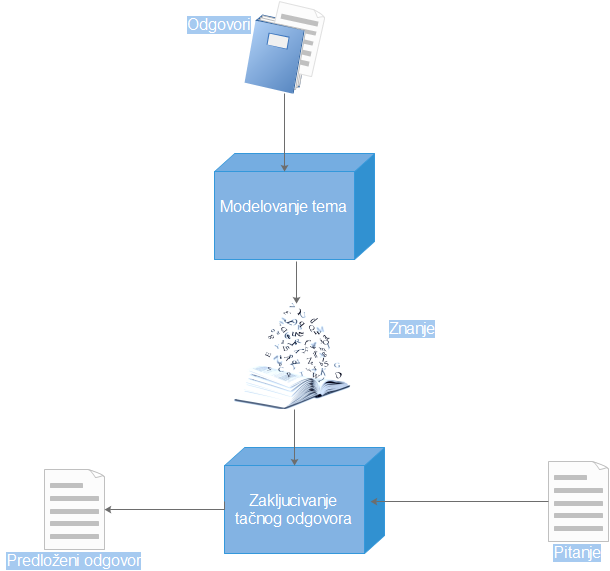
\includegraphics[scale=0.9]{./Slike/slika37.png} 
	\caption{Ток решења}
	\label{fig:slika1}
\end{figure}


\section{Мерење сличности}

Мерење сличности је од суштинске важности за одабирање одговора на постваљено питање. Она утиче на прецизност решења, брзину извршавања, меморијске захтеве итд. У раду су испитане три мере сличности од којих је мера заснована на вероватноћи дале најбоље резултате.


\subsection{Косинусна сличност}

Један од излаза алгоритма тема је и расподела тема по документима. Такође, за сваки нови документ, могуће је предвидети расподелу по темама. Дакле, пошто се вектор расподела по темама увек може направити, корисно их је искористити као меру сличности два документа.
%MILOS: Ово нису праве, него дужи. Замени свуда где треба. 
Вектор расподеле по темама, дужине $n$, може се замислити  као права у $n$-димензионаланом простору. Дакле, вектор питања и вектор одговора могу се замислити као две праве у $n$-димензионаланом. Што су те две праве "ближе" једна другој, односно што је угао између њих ближи нули, то су питање и одговор сличнији. 
Пошто се ради о расподелама, максимална вредност коју може да узме нека координата овако дефинисаног вектора је 1, док је минимална вредност 0, што значи да се обе праве налазе у првом квадранту. Дакле, максимални угао који два вектора могу да граде је 90 степени и, у смислу косинусне мере, означава да су документи потпуно различити.
Близина праве питања и праве одговора означава сличну расподелу по темама. Ако се узме у обзир полазна претпоставка да питање и одговор говоре о истим темама, постаје јасно због чега се угао између ових правих може узети за меру сличности два документа.

Ради илустрације, следи један упрошћен и, према томе, нереалан пример. 
Нека је скуп свих могућих речи састављен од три речи: \textit{reč1, reč2, reč3} и нека су дате три реченице састављене од поменутих речи: \textit{rečenica1, rečenica2, rečenica3}. Дате реченице се могу графички представити као праве (Слика 5.2).

\begin{figure}[H]
    \centering
   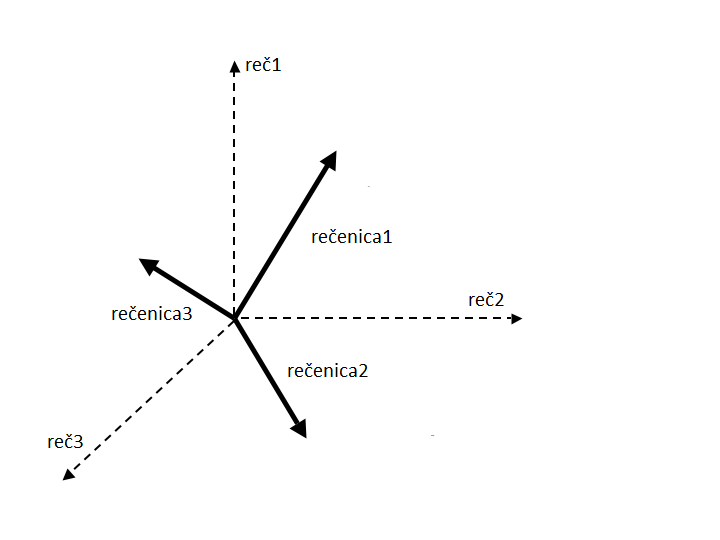
\includegraphics[scale=0.3]{./Slike/kosinusna.png} 
	\caption{Графички приказ косинусне сличности}
	\label{fig:slika1}
\end{figure}

Угао између сваке две праве представља меру сличности реченица.

Уместо мерења угла између два вектора, практичније је мерити косинус тог угла. 
Косинус угла који заклапају два вектора може се одредити следећом формулом :


$$ cos\theta = \frac{\overrightarrow{a}\cdot \overrightarrow{b}}{\Vert\overrightarrow{a}\Vert\overrightarrow{b}\Vert} $$

Претходна формула следи директно из дефиниције \textbf{скаларног производа} два вектора.


\subsection{Мерење сличности према лексичкој и тематској сличности}

Поред теметске сличности докумената, и лексичка сличност може бити важна. На пример, уколико се у одговору појављују исте речи као и у питању, \textbf{вероватније} је да је тај одговор ближи тачном одговору него одговор који нема заједничких речи са питањем. Наравно, могу се наћи примери у којима ово не важи. Али, исто тако, могуће је пронаћи примере у којима одговор и питање нису тематски слични - нпр. питање је уско специјализовано док је одговор теметски недефинисан. Према томе, знајући да обе мере сличности не морају увек да гарантују одабир правог одговора, уз одговорајући ризик, може се испитати утицај комбинације ове две мере на одабир одговора. 

Поставља се питање на који начин измерити лексичку сличност два документа тј. питања и одговора. Једно од решења би било једноставно бројање истих речи. Међутим, како је циљ испитати утицај \textbf{комбинације} лексичке и тематске сличности, ово решење се не може прихватити као одговарајуће. Разлог томе је што је лексичка сличност два документа измерена на овај начин \textbf{увек константна}, док се тематска сличност докумената разликује зависно од параметара модела. 	

Други начин мерења лексичке сличности докумената може се добити мерењем лексичке сличности \textbf{тема}.
Пошто се тема математички представља као функција расподеле над скупом свих речи, то сигурно за сваку реч из документа постоје вероватноће са којима свака тема садржи дату реч. Према томе, за сваки документ је могуће саставити $K$ вектора, где је $K$ укупан број тема, при чему $i$-ти вектор садржи вероватноће припадања речи документа  $i$-тој теми. \footnote{Ово се може гарантовати за сваку реч из одговора обзиром да је над скупом свих одговра изграђен модел. Међутим, може се догодити да се у питању појави реч која не постоји у корпусу модела. Вероватноће те речи у свим темама је тада нула.} Формалније, $i$-ти вектор се може записати као:

\begin{equation}
p_q^{(i)} = p(w_q \mid i,\phi^{(i)}),
\end{equation}

при чему је скуп речи документа дат са  $w_q = (w_1,w_2,..,,w_{|q|})$, док је $\phi^{(i)}$ расподела речи унутар  $i$-те теме. 
Дакле, вектор $p_q^{(i)}$ се формира тако што се за сваку реч из документа пронађе вероватноћа припадања те речи  $i$-тој теми, тј. важи да је 
$p_q^{(i)} = (\phi_{w_1}^{(i)},\phi_{w_2}^{(i)} ... ,\phi_{w_|q|}^{(i)}).$

Нека је одабрана тема  $i$. Да би се измерила лексичка сличност питања и одговора унутар ове теме, потребно је формирати описане векторе за оба документа. Димензије ова два вектора треба да буду исте и једнаке укупном броју различитих речи у корпусу. При томе, вероватноће оних речи из корпуса које не припадају документу ће у  векторима бити постављене на нулу.  Исто тако, треба водити рачуна да редослед навођења речи (тј. њихових вероватноћа) у оба вектора буде исти. То значи да ако је нпр. вероватноћа речи \textit{математика} у првом вектору наведена на трећој позицији, тада се на трећој позицији у другом вектору налази такође вероватноћа за реч \textit{математика}. 

Сличност ова два вектора може да се мери на више начина. У раду је коришћена косинусна мера сличности ,док је у раду \cite{tm2} коришћена Јенсен-Шенонова сличност. Дакле, лексичка сличност два документа у $i$-тој теми може се представити као:

$$
W(p_{pitanje}^{(i)},p_{odgovor}^{(i)}) = kosinusna_slicnost(p_{pitanje}^{(i)},p_{odgovor}^{(i)}).
$$

Укупна лексичка сличност питања и одговора се може дефинисати као:

$$
slicnost_1(pitanje,odgovor) = \frac{1}{K}\sum_{k=1}^K W(p_{pitanje}^{(k)},p_{odgovor}^{(k)}).
$$


На овај начин је измерена лексичка мера сличности између питања и одговора. Даље, потребно је дефинисати тематску сличност питања и одговора. Она се дефинише као косинусна сличност расподеле тема унутар питања и одговора (већ опшисана косинусна мера сличности). Дакле:

$$
slicnost_2(pitanje,odgovor) =kosinusnaSlicnost(\theta_pitanje,\theta_odgovor)).
$$

Коначно, сличност питања и одговора се дефинише као:

$$
slicnost(pitanje,odgovor) = slicnost_1(pitanje,odgovor)*slicnost_2(pitanje,odgovor).
$$

Ова мера је у пракси показала јако добре резулате. Међутим, битан недостатак јој је велика сложеност. Најпре, за свако питање и за сваки одговор потребно је проћи кроз све теме. Ово је већ сложеност $O(n^3)$ која је неприхватиљива у оваквој врсти проблема. Поред временске сложености, и просторна сложеност овог решења није мала. Наиме, за сваку тему мора се чувати (или стално изводити) расподела по свим речима. Величина корпуса може бити велика, па је ове структуре готово немогуће чувати у меморији. 
Због велике сложености, ова мера није испитана детаљно као косинусна мера, па су резултати добијени овом мером прилично непоуздани и сасвим оквирни. 
Она није погодна за решавање типова проблема у којима величина улзаног скупа може достићи и 20 000 докумената. Међутим, при мањем броју докумената, њена просторна и временска сложеност може да се компензује прецизношћу која се њоме добија. Подробнија испитивања ове мере нису рађена у  раду, а више о једној варијанти ове мере може се наћи у \cite{tm2}.

\subsection{Мерење сличности према предвиђеној вероватноћи}

Главни резулатати алгоритма моделовања тема су две расподеле - расподела речи по темама и расподела тема по документима. Ове две расподеле могу да се употребе како би се одредила сличност два документа.

Нека је дат документ $D$ и нека су познате $\theta_D$ -расподела тема унутар тог документа и $\phi$- расподеле речи унутатар свих тема. Тада се вероватноћа припадања неке речи $w$ документу $D$ може изразити као:

\begin{equation}
P_{lda}(w \mid D) = \sum_{z=1}^{K} P(w \mid z)P(z \mid \theta_D).
\end{equation}

при чему: \\

$ P(w \mid z)$ означава вероватноћу речи $w$ унутар теме $z$. Обзиром да речи са различитим вероватноћама припадају различитим темама и да је хиперпараметар Дирихлеове расподеле за расподелу речи над темама $\beta$, ова вероватноћа се изражава као условна, под условом $z$ и $\beta$. Хиперпараметар $\beta$ се подразумева, обзиром на начин како је модел направљен, тако да се и при писању може изоставити.\\
$P(z \mid \theta_D)$- означава вероватноћу са којом се тема $z$ јавља у документу $D$. Из сличних разлога као и код претходног чиниоца, ова вероватноћа се изражава као условна под условом $\theta_D$ и $\alpha$,  с тим што се $\alpha$ подразумева па се и не пише.

Дакле, формулом (5.2) може се прерачунати колико је вероватно да реч $w$ припада документу $D$. Ово се још може посматрати и као вероватноћа да је реч $w$ генерисана документом $D$.

Имајући ово у виду, може се сада дефинисати и вероватноћа да скуп речи припада документу  $D$, и то као:

\begin{equation}
P_{lda}(Q \mid D) = \prod_{w \in Q} p_{lda}(w \mid D).
\end{equation}

Претходна једнакост у ствари дефинише вероватноћу да је скуп речи генирасан документом $D$. Узимајући специјално да је тај скуп речи питање које се поставља систему, једнакост се може протумачити и као вероватноћа генерисања постављеног питања из датог одговора. \textbf{Вероватноћу генерисања} треба схватити као могућност извлачења речи питања из одговора.  Што је ова вероватноћа већа, већа је и могућност да питање и одговор говоре о истим стварима, те да посматрани одговор може бити тражени одговор на постављено питање.

Вероватноћа припадања речи $w$ неком документу $D$ се, поред формуле (5.2) може посматрати и из угла класичне вероватноће. Дакле, веровтаноћа да ће се реч $w$ наћи у документу $D$ једнака је укупном броју појављивања речи $w$ у том документу подељено са укупним бројем речи документа, односно:

\begin{equation}
P(w \mid D) = \frac{f_{w,D}}{|D|},
\end{equation}

где је $f_{w,D}$ број појављивања речи у документу док је $|D|$ укупан број речи у документу.

Обзиром да реч $w$ може бити било која реч, није нужно да она припада документу $D$. Дакле, може да се деси да ова вероватноћа буде нулта. Имајући у виду формулу (5.3), овако нешто је апсолутно неприхватљиво, поготово код дужих питања. На пример, уколико постоји само једна реч која се налази у питању, а не налази у одговору, док се осталих, рецимо 100, поклапају, то би резултовало вероватноћом  нула за генерисање питања из текста одговора. Овако нешто, наравно, не може да буде тачно.
Овај проблем може се решити увеђењем \textbf{псеудо појављивања}. 
Псеудо појављивања представљају број појављивања који се узима као подразумевани уколико се реч питања не налази у тексту одговора. На овај начин, свакој речи питања ће се доделити нека вероватноћа, која није нула, али је ипак довољно мала да ће се велико непоклапање речи између два документа одразити на резултат. Псеудо појављивања могу се увести на више начина. У конкретном раду, формула (5.4) замењена је формулом (5.5):

\begin{equation}
P(w \mid D) = \frac{f_{w,D} + \mu\frac{c_{w_i}}{|C|}}{|D|+\mu},
\end{equation}

где је\\
$\mu$ параметар који се експериментално одређује и представља псеудо појављивање,\\
$C$ је ознака укупног корпуса речи добијеног из свох одговора,
\\
$c_{w_i}$ - појављивање речи у корпусу.

Ни овакво решење није без мане. Наиме, и даље може да се деси да вероватноћа (5.3) буде једнака нулчи. То је случај када се у тексту питања појављује реч која се није нашла \textbf{ни у једном} од одговора. Међутим, овакви случајеви су ретки, поготово код већих скупова улазних података. Међутим, ако се то и деси, таквој речи, уместо вероватноће срачунате на било који од описаних начина се додељује вредност хиперпараметра $\beta$. Ова вредност узета је зато што се у алгоритму моделовања тема управо она додељује свим речима у оквиру свих тема у нултој итерацији. Та вредност сигурно није нула, али је довољно мала како би утицала на резултат.

Једнакостима (5.5) и (5.2) дефинисане су вероватноће припадања неке речи одређеном документу, али са различитим физичким смислом. Једнакост (5.2) дефинише тематску сличност, док једнакост (5.5) дефинише лексичку сличност. Међутим, ове две сличности не морају увек да буду подједнако важне, иако су обе значајне. Због тога би требало да постоји могућност контролисања удела са којим ове две сличности улазе у крајњу процену сличности. У конкретном раду, овај проблем решен је додавањем додатног параметра $\lambda$. Што је његова вредност већа, то је лексичка сличност докумената важнија и обрнуто.

Поменуте вероватноће могу се уклопити тако да заједно граде меру сличности. У конкретном раду, вероватноћа генерисања речи из текста дата је са:
\begin{equation}
P(w \mid D)  = \lambda(\frac{f_{w,D} + \mu\frac{c_{w_i}}{|C|}}{|D|+\mu}) + (1-\lambda)(\sum_{z=1}^{K} P(w \mid z)P(z \mid \theta_D)).
\end{equation}

Мера укупне сличности два документа се и даље рачуна преко (5.3).
За вредности парамтера $\lambda$ и $\mu$  могу се узети било које вредности, уз ограничење $\lambda \leq 1$. За потребе рада, експериментално су одређене врености $\mu = 200$ и $\lambda = 0.2$.

	
\chapter{Развој решења}

Циљ мастер рада био је \textit{истраживање могућности} примене алгоритама моделовања тема у основној верзији  при предлагању одговора на питање постављено природним језиком. Стога, алгоритам моделовања тема није развијан од почетка већ се користило готово решење у оквиру софтверског пакета \textit{Mallet}.
Основни разлог развоја софтверског окружења налази се у потреби тестирања различитих претпоставки везаних за примену алгоритама моделовања тема у задатом проблему. Стога је развојено, у програмској језику Java, неколико класа које су имале са циљ обезбеђивање лаког и једноставног тестирања претпоставки.

Анализа резултата тестирања хипотеза вршила се помоћу Matlab-а и  Microsoft Excel програма.
 
\section{Општи преглед пакета Mallet}

Софтверски пакет \textit{Mallet} је софтвер \textbf{отвореног кода - енг. open source} и представља скуп алгоритама машинског учења оријентисаних на текстуалне податке. Обухвата различите врсте алгоритама за  моделовања тема (енг. topic modeling), кластеровање (енг. clustering), класификацију (енг. classification), статистичке обраде природног језика (енг. statistical natural language processing) итд. Сви алгоритми развијени су у Java програмском језику

Алгоритам моделовања тема у овом пакету има две реализације. Основна верзија, која је коришћена у овом раду, представља имплементацију LDA-a (енг. Latent Dirichlet Allocation) Гибсовим узорковањем. Друга верзија предстваља хијерархијски LDA-a. Примена хијерархијске врста алгоритма моделовања тема није била предмет овог рада али би било интересантно испитати те могућности у будућем раду.

Софтверски пакет \textit{Mallet} може се користити на два начина : конзолно - коришћењем предефинисаних команди, или се, обзиром на то да је код јавно доступан, сам код може убацити у постојећи пројекат. Пошто је циљ истраживања био специфичан и захтевао извесне модификације основне верзије решења у пакету  \textit{Mallet}, у раду је коришћена друга опција.

 
\subsection{Подаци у Mallet-у}

 

\textit{Mallet} користи објекте класе \textbf{Instance} за представљање података при чему  сваки засебан објекат  представља посебан документ. У конкретном случају под \textbf{документом} се подразумева текст питања или одговора.  Дакле, један објекст класе \textbf{Instance}  представља или једно питање или један одговор.

Превођење "`сирових"' података у објекте класе  \textbf{Instance} представља предпроцесирање података за све алгоритме пакета \textit{Mallet} и неопходан је корак при коришћењу било ког од тих алгоритама. 

Превођење података у објекте класе \textbf{Instance}, обзиром на конструкторе, могло би да се посматра као тривијалан посао. Међутим, обзиром на специфичне захтеве исраживања, потребно је укључити и све кораке предпроцесирања који су наведени у претходом поглављу. За тако нешто је коришћена класа \textit{Pipe}, такође из пакета \textit{Mallet}.

\textit{Pipe} је апстрактна класа и представља надкласу за све класе које се користе за модификовање објекста  класе \textbf{Instance} у предпроцесирању. У пакету \textit{Mallet} постоји неколико предефинисаних класа које врше неке од трансформација поменутих у претходном поглављу - нпр. уклањање HTML ознака (класа CharSequenceRemoveHTML), превођење у мала слова ( класа  CharSequenceLowercase() ), формирање токена од текста (класа CharSequence2TokenSequence )  или уклањање често коришћених речи ( класа TokenSequenceRemoveStopwords ).
Поред поменутих, већ уграђених класа, за потребе рада дописане су још и :
\begin{itemize}
\item класа за уклањање наставака речи - PipeStem
\item класа за свођење на коренску реч - StanfordLemmatizer
\item класа за убацивање синонима - InsertSynonyms
\end{itemize}

У додатку су дате неке од тих класа.

Пошто предпроцесирање најчешће захтева више од једне трансформације, пракса је формирање низа објеката типа \textit{Pipe} који секвенцијално врше трансформацију објекта класе \textbf{Instance}. Тај низ најчешће се формира објекстом класе \textit{SerialPipe}.

Обзиром на то да улазни подаци у било који алгоритам машинског учења најчешће нису поједнични документи већ скупови документа, од интереса је и класа  \textit{InstanceList} којом се једноставно  апстрахује  скуп докумената. Објекти ове класе садрже групу\textbf{Instance} објеката над којима су извршене исте трансформације (исти SerialPipe).

\subsection{Алгоритам моделовања тема у Mallet-у }

Алгоритам моделовања тема у Mallet-у представља имплементацију LDA-а (Latent Dirichlet Allocation) преко Гибсовог узорковања. Постоји више имплементација од којих је \textit{ParallelTopicModel} најјефикаснија. У тој класи је реализован основни LDA-а алгоритам коришћењем Гибсовог узорковања. Перформансе су повећане паралелизацијом преко нити. Овај класа је коришћена у истраживању.

При моделовању тема следећи параметри су од интереса :

\begin{itemize}
\item број тема
\item број итерација
\item хиперараметри
\end{itemize}

Вредности ових параметара се задају пре моделовања тема и од њих директно зависи решење. 
У истраживању највећи акцент је био на проналажењу оптималних вредности ових параметара и то пре свега броја тема и итерација. Вредности хиперпараметара су фиксиране тако да, што  релистичније описију знања о полазном скупу података. То подразумева подједнаку вероватноћу свих тема у оквиру докумената као и подједнаку вероватноћу свих речи у оквиру свих тема. 

Приликом проналажење оптималне вредности броја тема и итерација прибегло се похлепном решењу тј. испитивању свох могућих комбинација. Разлог за такав приступ, поред проналажења оптималних вредности параметара, био је и испитивање \textbf{тренда} перформанси модела.   Обзиром да је то временски изузетно захтеван посао, овај део истраживања одрађен је коришћењем \textbf{кластера}. У додатку је пример скрипте којом се покрећу послови на кластеру. 

Процес моделовања тема извршава се у оквиру методе \textit{estimate} класе ParallelTopicModel где се, у одређеном броју итерација, врши Гибсово узороковање по познатим обрасцима. Овај процес још се назива и \textbf{тренирање модела}. Крајњи резултат представља \textbf{истрениран модел} који у себи садржи информације о :
\begin{itemize}
\item расподели тема унутар сваког документа
\item расподели речи унутар сваке теме
\end{itemize}


Једна од интересантних ствари које се на основу ових информација могу закључити је и расподела тема унутар \textbf{новог} документа тј. документа који није коришћен при тренирању. То се постиже класом \textit{TopicInferencer} која симулира  у одређеном броју итерација претходни процес тренирања, стим што се промене односе само на нови документ. Дакле, овим није могуће накнадно тренирати већ истрениран модел, али је из података истренираног модела могуће наслутити расподелу тема на невиђеном документу.

Поред наведене класе, у Mallet-у постоји и \textit{SimpleLDA}  која такође имплементира LDA-а алгоритам коришћењем Гибсовог узорковања али у верзији која није оптимизована. Због бољег разумевања суштине рада алгоритма, у почетној фази истраживања коришћена је ова класа. Касније се због перформанси прешло на решење у оквиру класе  ParallelTopicModel.


\section{Опис решења}

Основни циљ развоја софтвера био је селектовање одговора који најбоље одговара на постављено питање. Идеја решења је изградња \textbf{модела тема} над свим одговорима чиме би се добио истрениран модел који поседује знање о расподели тема над документима као и расподели речи унутар тема. Затим се за  постављено питање процењује расподела тема над њим и мери се \textbf{сличност} тог питања са свим одговорима у бази. Најсличнији одговор се проглашава одговором на постављено питање, при чему се кориснику предлаже 30 највероватнијих одговора.

У улазне податке спадају листа питања и листа одговора на та питања. Дакле, зна се који одговор припада ком питању, односно може се установити да ли је програм адекватно проценио који је прави одговор. Стога се за оцену квалитета решења може узети \textbf{број тачних одговора} који су се јавили у првих 10, 20 или 30 предложених. 

За мерење сличности питања и одговора коришћено је неколико метода :

\begin{itemize}
\item Косинусна сличност расподеле по темама - ово је најједноставнија мера сличности. Пошто је познат број тема, сваки документ се може представити вектором дужине броја тема. На $i-том$ месту у сваком вектору налази се вероватноћа, односно присуство $i-те$ теме у том документу. Косинусна сличност овакава два вектора представља меру сличности одговарајућих докумената. Што су расподеле по темама сличније, то ће мера сличности бити ближа 1. Основни разлог за овакво решење била је претпоставка да су питање и прави одговор \textbf{тематски} јако слични

\item Сума косинусних сличности расподела речи - обзиром да је позната расподела речи по темама могуће је  за сваку тему формирати вектор који за сваку реч из документа садржи вероватноћу те речи у одговарајућој теми. На овај начин се формирају два вектора, један за питање а други за одговор. Косинусна сличност ових вектора рачуна се за сваку тему а њихова сума представља меру сличности докумената

\item Вероватноћа генерисања питања на основу одговора и њене варијације - обзиром да је позната расподела тема по документима као и расподела речи унутар тема, једноставно се може прерачунати вероватноћа генерисања текста питња на основу текста одговора. Та вероватноћа представља меру сличности ова два документа.Варијације ове теме односе се на прерачунавање вероватноће. У раду су испитана још два додатна начина али је основна верзија показала најбоље резултате.

\end{itemize}

Испитане мере сличности разликују се по прецизности, брзини рада и меморијским захтевима. Испоставило се да су  за примену на већи скуп података погодна прва и трећа ( са варијантама) метода .

Идејни ток решења може се представити  дијаграмом као на слици 3.1:

\begin{figure}[H]
    \centering
   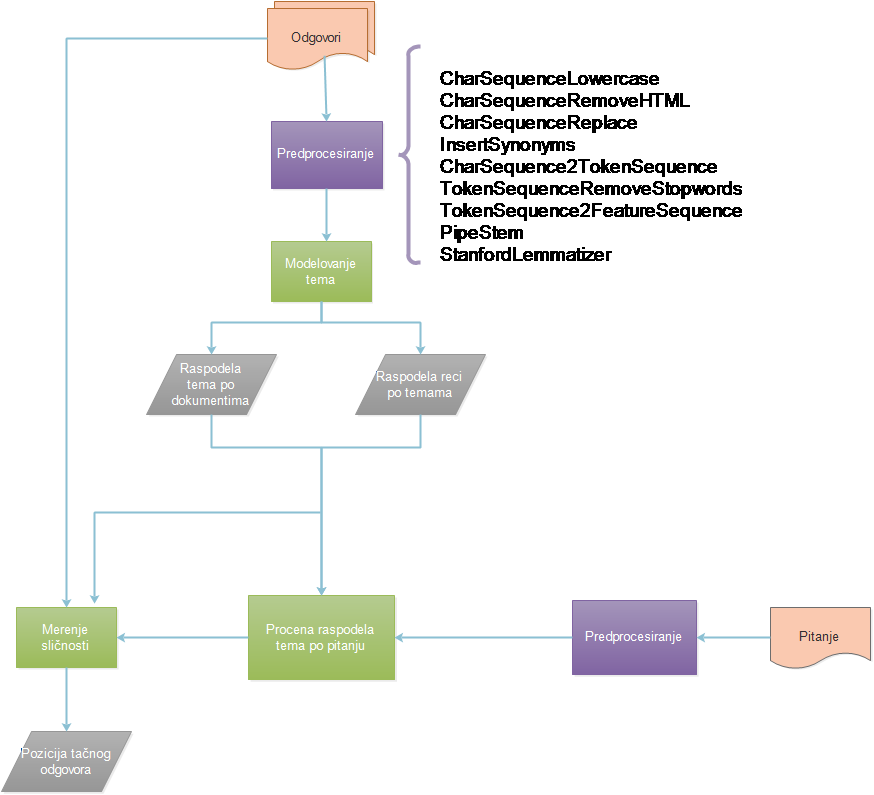
\includegraphics[scale=0.7]{./Slike/slika38.png} 
	\caption{Ток решења}
	\label{fig:slika1}
\end{figure}


Важно је приметити да се у предпроцесирању не морају извршити све наведене трансформације нити у назаначеном редоследу. Одабир подскупа транформација директно утиче на резулат док редослед извршавања мора имати смислени ток. У конкретном истраживању, наведене трансформације су извршаване у датом редоследу. Главни циљ је био испитивање утицаја синонима, стеминга и лемитизације на резултат, тако да су ове три транформације укљичиване и искључиване како би се испитале све могуће комбинације.

Исто тако, ради конзистентности решења, структура и редослед предпроцесирања питања и одговора морају бити \textbf{исти}. Из тог разлога су на дијаграму и обојени истом бојом.



\chapter{Решење проблема применом методе бројања речи}

Метода бројања речи једна је од једноставнијих метода којом  је могуће поредити два текстулана документа.  Основна претпоствка ове методе је да су документи ближи један другом уколико  имају више заједничких речи.  Оваква претпоствка иако делује сасвим основано, не мора увек да буде тачна. Истим скупом речи могу се описати потпуно различите ствари и тиме генерисати два текстулана документа која, по смислу, уопште нису слична. Иако су овакви примери бројни, ова метода је, пре свега, због једноставности имплементације широко прихваћена у системима за проналажења одговора на постављено питање.

У конкретном раду, метода бројања речи је коришћена као \textbf{компаративнно решење} у односу на решење применом алгоритма моделовања тема. 

\section{Опис решења методом бројања речи}

Улаз у алгоритам су група питања и група одговора, при чему се за свако питање унапред зна који одговор из дата групе одговора представаља тачан одговор. Решење методом бројања речи заснива се на мерењу сличности датог  питања са \textbf{сваким одговором} у бази одговора. Након тога, одговори се рангирају према израчунатој сличности. Позиција тачног одговра у тој хијерархији свих одговора предствља излаз који алгоритам даје за свако постављено питање. 

Да би резултати ове методе могли да се пореде са резултатима претходно развијеног решења, неопходно је обезбедити \textbf{исте улазне податке}. Обизором на начин предпроцесирања у решењу базираном на моделовању тема, да би се обезбедили идентични улази коришћен је исти приступ предпроцесирању. То подразумева развој класе која, након предпроцесирања података за коришћење у алгоритму моделовања тема, те податке уписује на екстерни диск. Овим је обезбеђен апсолутно исти улаз и за компаративно решење.

Ради лакшег рачунања сличности докумената. сваки документ је представљен као вектор, тј. као низ неких нумеричкоих вредности. Трансформације текстуалног документа у вектор може се обавити на више начина. У раду су кориштена два приступа :
\begin{itemize}
\item једноставно бројање речи - Сваки документ представљен је као један низ. Свакој речи документа се додељује један природан број који представља индекс у том низу, при чеми исте речи имају додељене исте бројеве. На тој позицији у низу налази се број појављивања те речи у документу. За мерење сличности два документа неопходно је обезбедити исто мапирање речи у природне бројеве. Ово значи да исти индекс у оба документа одговора истим речима.
\item коришћење популарне TF-IDF методе - вектори се формирају на исти начин као код класичног приступа бројањем речи стим што се нумеричка вредност у вектору рачуна по формулама TF-IDF методе.
\end{itemize}

За меру сличности два документа узета је \textbf{косинусна сличност} прерачунатих вектора.

\chapter{Преглед резултата}

Приликом израде  рада развијено је софтверско окружење којим су се тестирали различити приступи решавању задатог проблема. Пре свега овде се мисли на различите мере сличности које су тестиране.  Основна мера квалитета решења је \textbf{просечна позиција} тачног одговора у листи свих одговора. Што је просечна позиција нижа тј. ближа 1 то се решење сматра квалитетнијим, при чему се тежи да стандардна девијација буде што мања.
Поред просечне позиције, битне карактеристике решења су брзина рада и меморијски захтеви.

Свака од тестираних мера сличности има своје параметре који су у мањој или већој мери осетљиви на одабир корака  у предпроцесирању. Обзиром да се ради о алгоритму моделовања тема, у зависноти од мере, биће потребан различит број тема и итерација како би се постигло оптимално решење. Због тога је било неопходно испитати за сваки меру посебно како који кораци предпроцеситрања утичу и  које вредности параметара алгоритма моделовања тема су оптималне за ту меру.  

Прво тестирање решења проблема вршено је на скупу од 360 питања и 360 одговора преузетих са сајта \textit{stackexchange.com}. 


\section{Утицај броја тема и броја итерација на просечну позицију}

Обзором на то да расподела тема по документима, у мањој или већој мери, утиче на свако од тестираним мера, број тема представља битан параметар. Са малим бројем тема а на основу предложених мера, јако је тешко рангирати одговоре. Разлог томе је што ће се теме дефинисати према областима којима се баве документи. Према томе документи из исте области имаће сличне расподеле по темама а самим тим и приближно исту удаљеност од тестног документа односно питања. Због тога је неопходно да број тема буде довољно велики како би се овај проблем заобиша. 

Међутим, није добро узети ни превелики број тема. У том случају сви документи ће имати сличну расподелу по темама па ће и одстојање од тестног документа бити приближно исто. Ово директно утиче на просечну позицију сводећи је на број који је једнак $[\frac{brojDokumenata}{2}]$. Овако нешто може се видети на следећем графику \footnote{Ово тестирања  је рађено на самом почетку и то на полазном скупу од 150 докумената. Тај скуп је подскуп скупа на коме су вршена сва остала тестирања} :

		\begin{figure}[H]
    \centering
   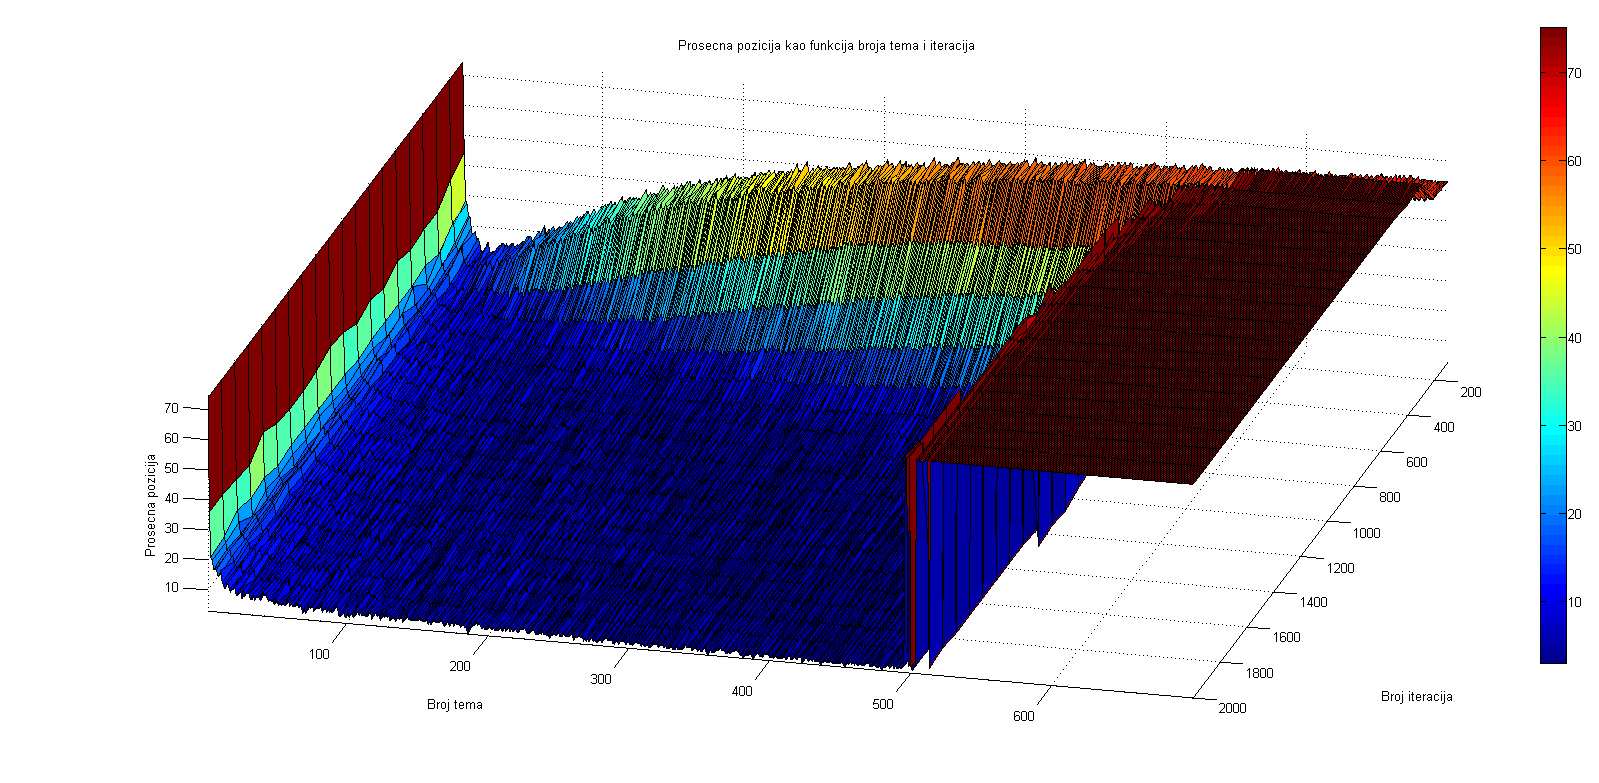
\includegraphics[scale=0.3]{./Slike/cutoff.png} 
	\caption{Зависност просечне позиције од броја тема и броја итерација}
	\label{fig:slika1}
\end{figure}


Прелаз на просечну позицију $[\frac{brojDokumenata}{2}$ ( у конкретном случају 74 јер је број докумената 150 ) је прилично груб. Разлог томе је што нису тестиране све вредности броја итерација него свака 100-та. Како je за потребе рада било довољно  уочити да се број тема не може бесконачно повећавати, ова појава даље није испитивана.


\section{Утицај корака предпроцесирања на просечну позицију}

Предпроцесирањем се \textbf{трансформише} текст улазних података како би био погоднији за обраду. Сама природа проблема намеће неке кораке предпроцесирања као неопходне. У њих спадају :

\begin{itemize}
\item превођење свих слова текста у мала слова - ова трансформација је неопходна како се не би  реч написана почетним великим словом и иста реч написана почетним малим словом третирали као две различите речи
\item уклањање HTML ознака - обзиром на порекло података, поред корисног текста, у документима се налазе и HTML ознаке које, са аспетка овог проблема, немају никаквог значаја.
\item уклањање свих неалфанумеричких карактера - овом трансформацијом се уклањају знакови интерпукције и специјални знакови који нису битни за решење овог проблема
\item уклањање често коришћених речи - оне не носе тематско значење, честе су у свим документима и представљју оптерећење при обради
\end{itemize}

Ове трансформације су се увек укључивале, без обзира на  меру сличности. Поред њих, додате су и стеминг, лемитизација и синоним трансформације у различитим комбинацијама. 


\subsection{Резултати без додатних трансформација}

Улазни подаци - и питања и одговори - трансформисани преко три описана корака предпроцесирања и то у редоследу :  превођење свих слова текста у мала слова, уклањање HTML ознака и уклањање често коришћених речи.

	\subsubsection{Косинусна сличност}
Уколико се за меру сличности одабере \textbf{косинусна} мера, просечна позиција тачног одговора директно зависи од параметара модела тј. од броја тема и броја итерација. Та зависност се може приказати следећим графиком. ( слика 8.2)
		\begin{figure}[H]
    \centering
   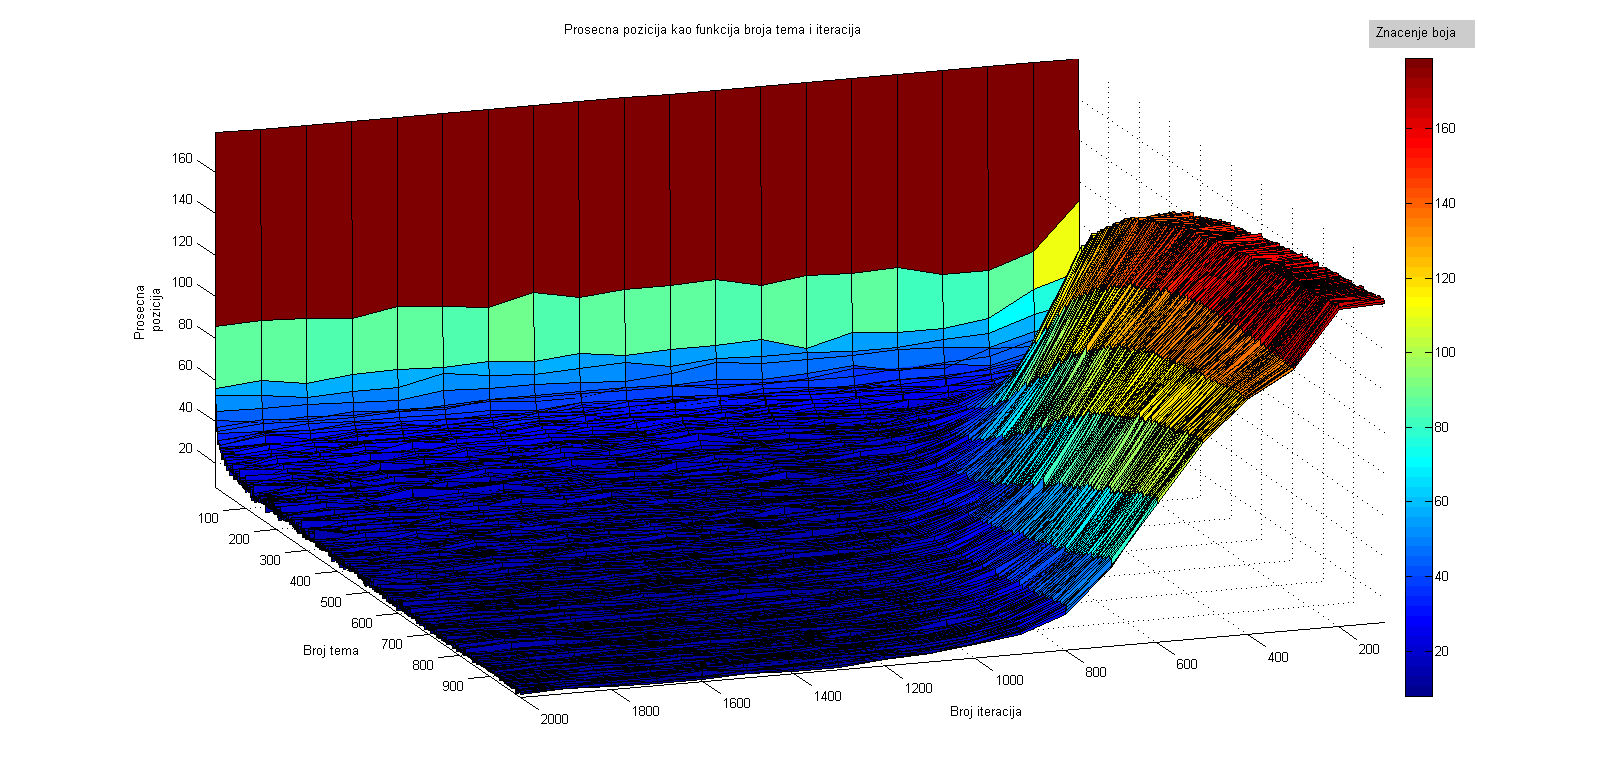
\includegraphics[scale=0.3]{./Slike/noStemNoSyn.png} 
	\caption{Зависност просечне позиције од броја тема и броја итерација}
	\label{fig:slika1}
\end{figure}

Минимална просечна позиција је \textbf{8} и добија се при више различитих комбинација параметара. Неке од комбинација су приказане у следећој табели

\begin{center}
\captionof{table}{Утицај броја тема и итерација на просечну позицију тачног одговора}
\begin{tabular}{|c|c|}
\hline
Број итерација & Број тема \\
\hline\hline
1200 & 693 \\
1400 & 756 \\
1400 & 820 \\
\hline
\end{tabular}

\end{center}

	\subsubsection{Мерење сличности према лексичкој и тематској сличности}
	
Уколико се за меру сличности одабере мера  \textbf{лексичке и теметске} сличности, просечна позиција такође директно зависи од параметра модела. Обзиром на временску и просторну сложеност ове мере, нису испитиване све могућности за параметре модела. График зависности просечне позиције од броја тема и итерација дат јена следећој слици (слика 8.3)

		\begin{figure}[H]
    \centering
   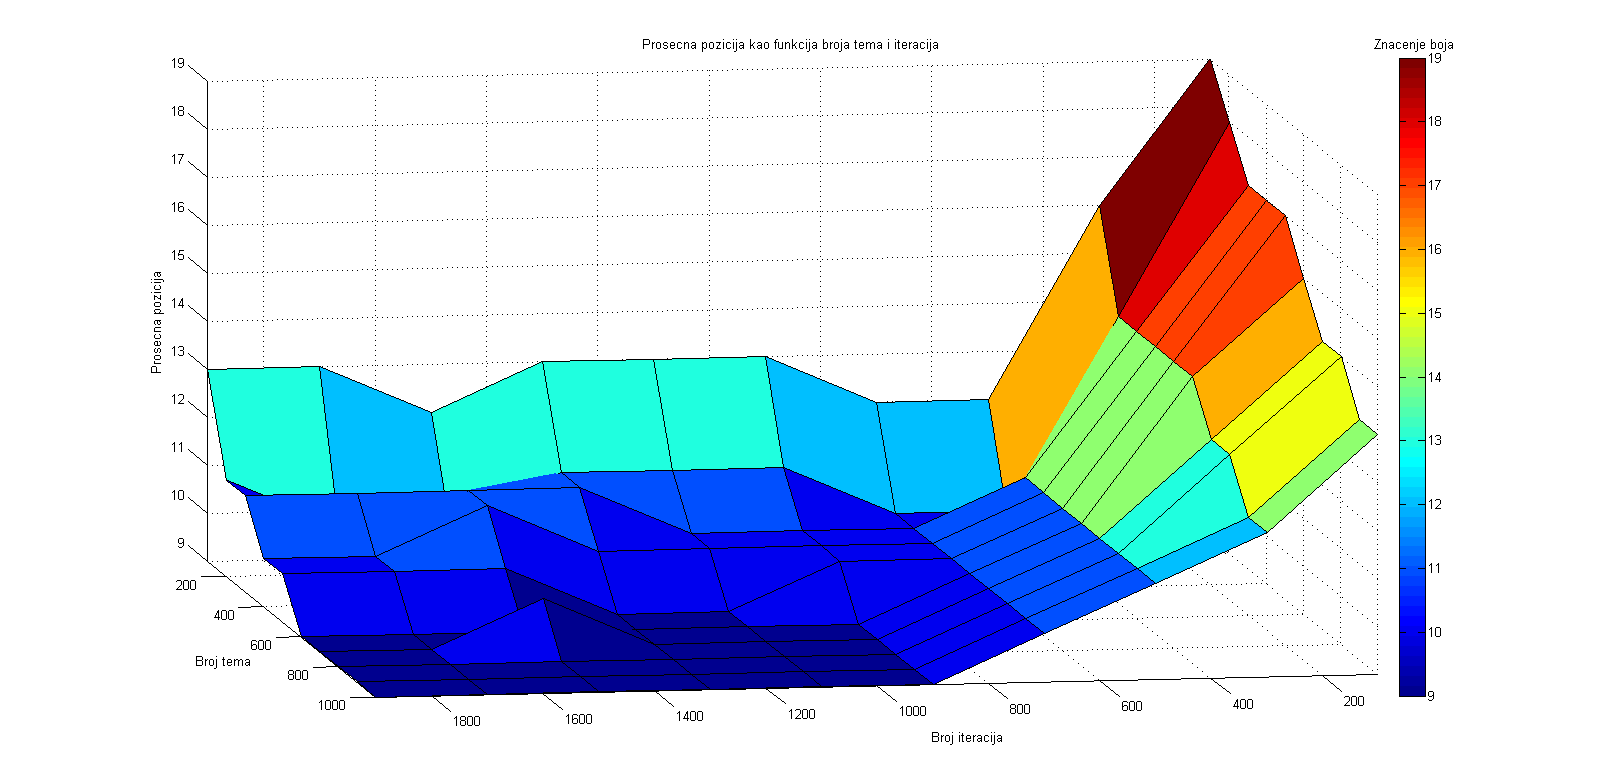
\includegraphics[scale=0.3]{./Slike/distnoStemNoSyn.png} 
	\caption{Зависност просечне позиције од броја тема и броја итерација}
	\label{fig:slika1}
\end{figure}

Минимална просечна позиција је \textbf{9} и добија се при више различитих комбинација параметара. Неке од комбинација су приказане у следећој табели

\begin{center}
\captionof{table}{Утицај броја тема и итерација на просечну позицију тачног одговора}
\begin{tabular}{|c|c|}
\hline
Број итерација & Број тема \\
\hline\hline
900 & 600 \\
900 & 700 \\
1100 & 500 \\
\hline
\end{tabular}

\end{center}


\subsection{Утицај стеминга на резултат}

Поред основне три трансформације, на улазне податке је примењене и стеминг модификација - уклњање наставака речи. Овим је полазни скуп података упрошћен јер је скуп различитих речи мањи. Без ове трансформације, једна иста реч у различитим родовима или временима се посматрала ралзличито што је довело до великог диверзитета у скупу речи ( на пример речи енг. think и енг. thinking су посматране као различите речи без обзира на исто основно значење речи ). 

\subsubsection{Косинусна сличност}



Утицај стеминга на просечну позицију  када се сличност мери косинусном сличношћу дат је на следећем графику( слика 8.4)

		\begin{figure}[H]
    \centering
   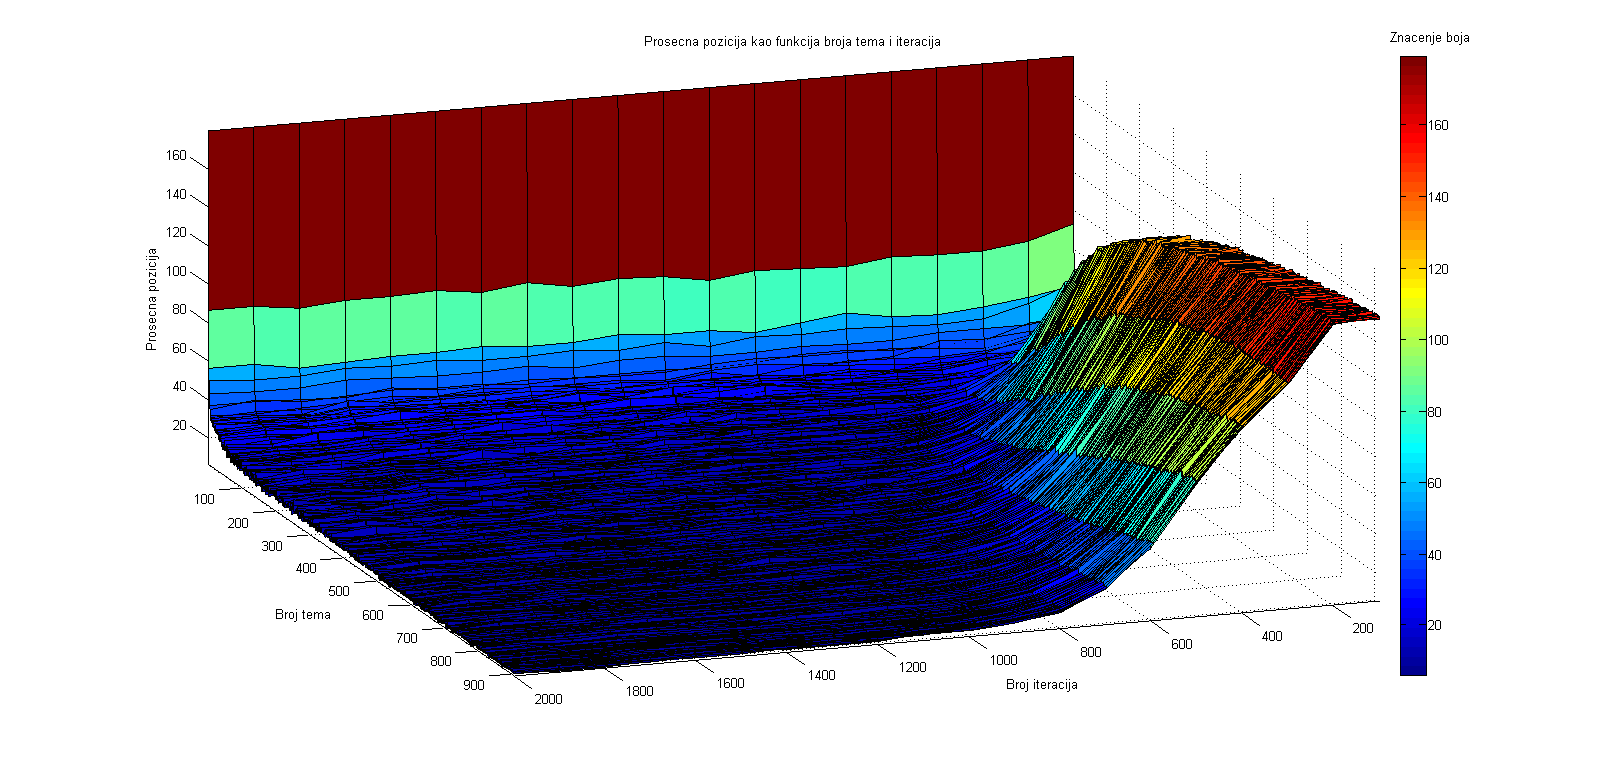
\includegraphics[scale=0.3]{./Slike/StemNoSyn.png} 
	\caption{Зависност просечне позиције од броја тема и броја итерација}
	\label{fig:slika1}
\end{figure}

Минимална просечна позиција је \textbf{6} и добија се при више различитих комбинација параметара. Неке од комбинација су приказане у следећој табели

\begin{center}
\captionof{table}{Утицај броја тема и итерација на просечну позицију тачног одговора}
\begin{tabular}{|c|c|}
\hline
Број итерација & Број тема \\
\hline\hline
1100 & 621 \\
1200 & 643 \\
1300 & 724 \\
\hline
\end{tabular}
\end{center}

Додавање стеминга утиче на нижу просечну позицију и на упрошћавање модела. Без примене стеминга, најједноставнији модел којим се постиже оптимална просечна позиција је био комбинација 1200 - 693 док је са стемингом то 1100 - 621. Дакле, додавањем и стеминга коришћењем мањег броја тема и у мање итерација постижу се бољи резултати. 


\subsubsection{Мерење сличности према лексичкој и тематској сличности}
	
Уколико се за меру сличности одабере мера  \textbf{лексичке и теметске} сличности, просечна позиција такође директно зависи од параметра модела. Обзиром на временску и просторну сложеност ове мере, нису испитиване све могућности за параметре модела. График зависности просечне позиције од броја тема и итерација дат јена следећој слици (слика 8.5)

		\begin{figure}[H]
    \centering
   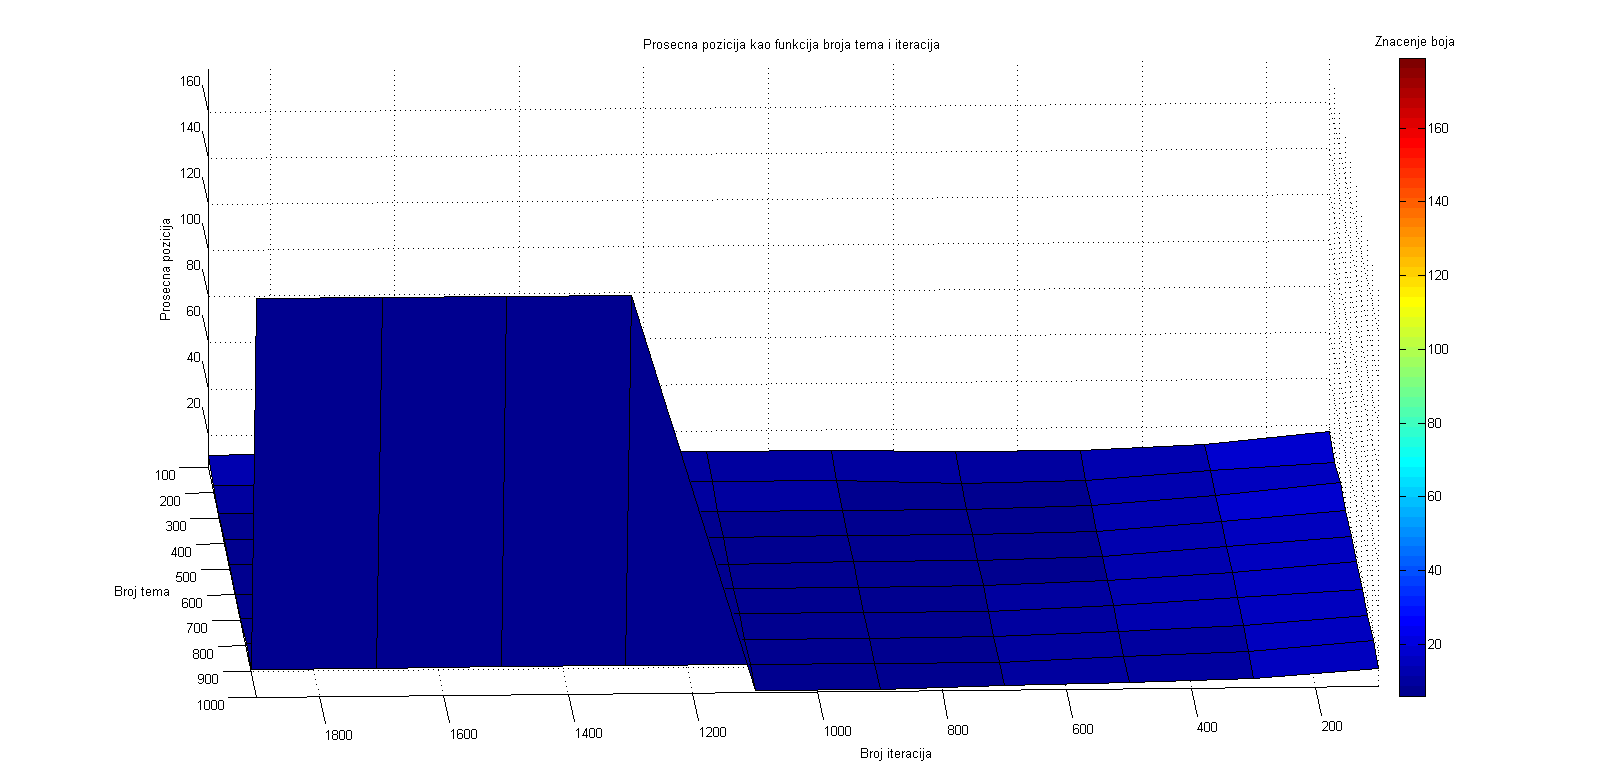
\includegraphics[scale=0.3]{./Slike/distStemNoSyn.png} 
	\caption{Зависност просечне позиције од броја тема и броја итерација}
	\label{fig:slika1}
\end{figure}

Минимална просечна позиција је \textbf{6} и добија се при више различитих комбинација параметара. Неке од комбинација су приказане у следећој табели

\begin{center}
\captionof{table}{Утицај броја тема и итерација на просечну позицију тачног одговора}
\begin{tabular}{|c|c|}
\hline
Број итерација & Број тема \\
\hline\hline
1100 & 500 \\
1300 & 600 \\
1300 & 800 \\
\hline
\end{tabular}

\end{center}


\subsection{Утицај лемитизације на резултат}

Лемитизација је процес свођења речи на \textbf{коренску} реч. Склањањем наставака речи могуће је пронаћи заједничку основу речи. Али, уколико реч мења облик у различитим лицима или временима, склањањем наставка речи, уколико уопше постоје, неће се добити иста реч. Лемитизацијом се овај проблем решева. На основу граматичких правила, препознаје се који основни облик реч и тим обликом замњује сепојављивање те речи у било којој форми. 




\subsubsection{Косинусна сличност}



Утицај лемитизације на просечну позицију  када се сличност мери косинусном сличношћу дат је на следећем графику( слика 8.6)

		\begin{figure}[H]
    \centering
   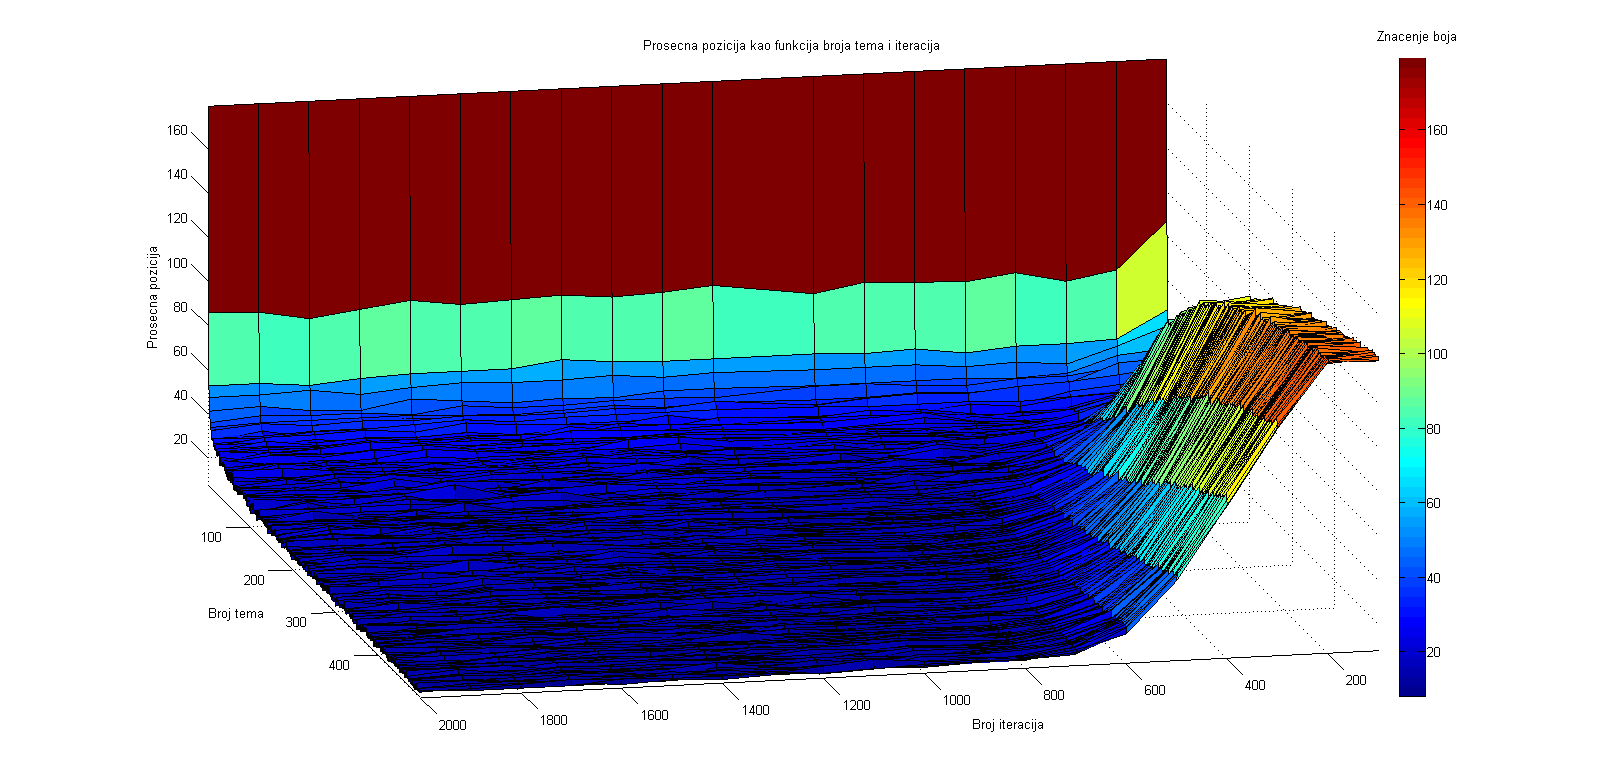
\includegraphics[scale=0.3]{./Slike/LemmNoSyn.png} 
	\caption{Зависност просечне позиције од броја тема и броја итерација}
	\label{fig:slika1}
\end{figure}

Минимална просечна позиција је \textbf{8} и добија се при више различитих комбинација параметара. Неке од комбинација су приказане у следећој табели

\begin{center}
\captionof{table}{Утицај броја тема и итерација на просечну позицију тачног одговора}
\begin{tabular}{|c|c|}
\hline
Број итерација & Број тема \\
\hline\hline
1300 & 481 \\
1300 & 486 \\
1500 & 481 \\
1600 & 477 \\
\hline
\end{tabular}
\end{center}

Може се закључити да лемитизација значајно утиче на поједностављивање модела. Најмања вредност просечне позције добије се коришћењем броја тема око  470 за разлику од основног модела где тај број износи преко 600.

Обзиром на то да лемитизација своди на коренску реч, мањи је диверзит скупа речи. Самим тим, моделу је теже да препозна прави одговор па је због тога просечна позиција више него просечна позиција која се добија употребом стеминга.



\subsubsection{Мерење сличности према лексичкој и тематској сличности}
	
Уколико се за меру сличности одабере мера  \textbf{лексичке и теметске} сличности, просечна позиција такође директно зависи од параметра модела. Обзиром на временску и просторну сложеност ове мере, нису испитиване све могућности за параметре модела. График зависности просечне позиције од броја тема и итерација дат јена следећој слици (слика 8.7)

		\begin{figure}[H]
    \centering
   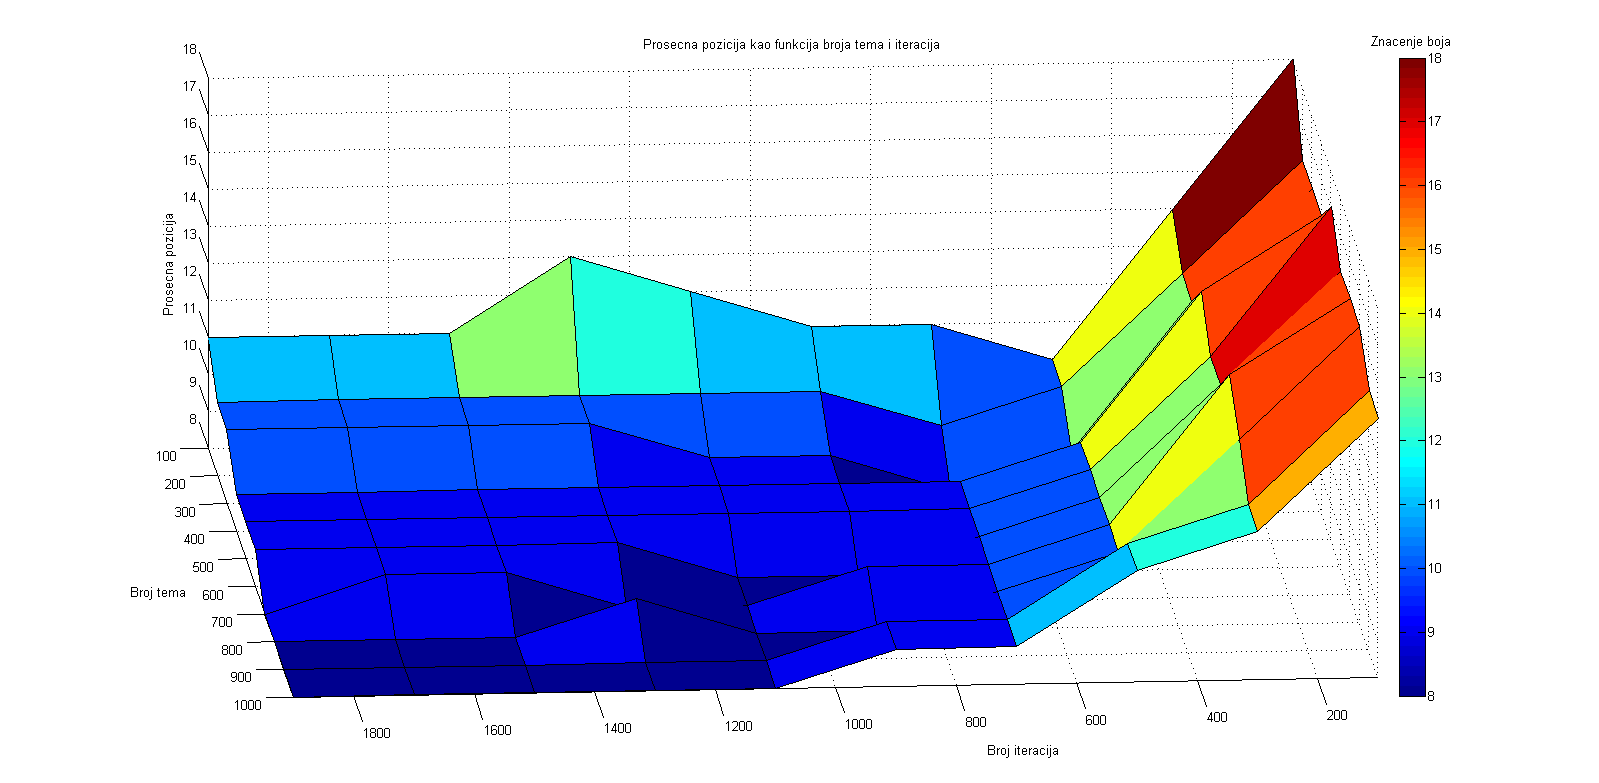
\includegraphics[scale=0.3]{./Slike/distLemNoSyn.png} 
	\caption{Зависност просечне позиције од броја тема и броја итерација}
	\label{fig:slika1}
\end{figure}

Минимална просечна позиција је \textbf{8} и добија се при више различитих комбинација параметара. Неке од комбинација су приказане у следећој табели

\begin{center}
\captionof{table}{Утицај броја тема и итерација на просечну позицију тачног одговора}
\begin{tabular}{|c|c|}
\hline
Број итерација & Број тема \\
\hline\hline
700 & 300 \\
900 & 600 \\
900 & 800 \\
\hline
\end{tabular}

\end{center}




\subsection{Утицај додавања синонима на резултат}

Додавање синонима речи има за циљ боље тематско одвајање. Наиме, уколико се свакој речи придода неколико синонима, претпоставља се да ће теметско одвајање бити једноставније. Основни разлог за увођење ове врсте трансформација била чињеница да  човек поузданије закључује "`о чему се ради"' у неком тексту уколико му се наведе неколико синонима за кључне речи. Обзиром да се ниједна реч не потенцира свакој речи је додат неки број синонима. Будући да додавање синонима директно утиче на перформансе система, у конкретном раду је одлучено да тај број буде 5.

 


\subsubsection{Косинусна сличност}



Утицај  на додавања синонима на просечну позицију  када се сличност мери косинусном сличношћу дат је на следећем графику( слика 8.8)

		\begin{figure}[H]
    \centering
   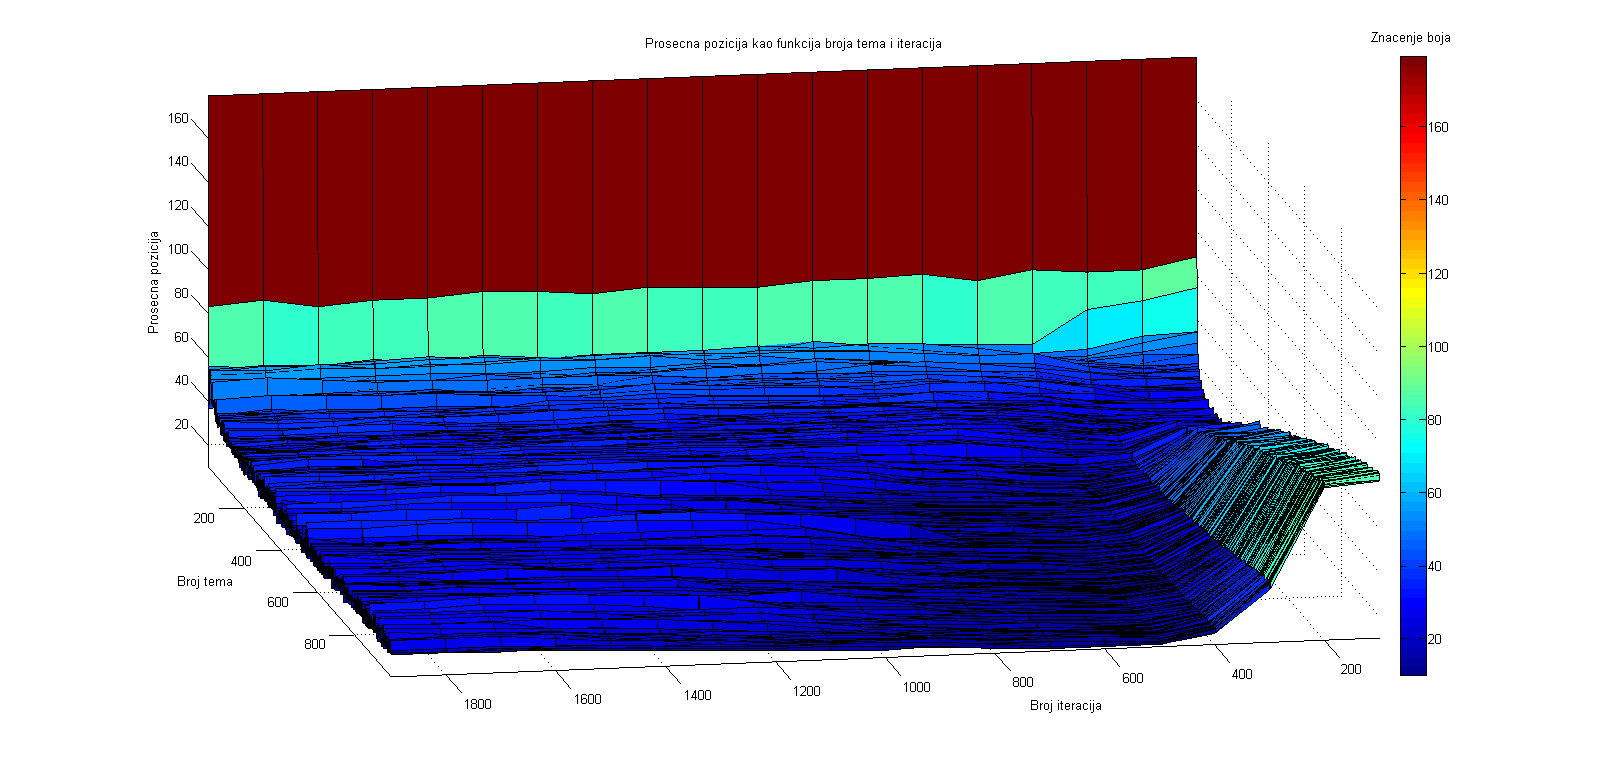
\includegraphics[scale=0.3]{./Slike/NoStemmSyn.png} 
	\caption{Зависност просечне позиције од броја тема и броја итерација}
	\label{fig:slika1}
\end{figure}

Минимална просечна позиција је \textbf{10} и добија се при више различитих комбинација параметара. Неке од комбинација су приказане у следећој табели

\begin{center}
\captionof{table}{Утицај броја тема и итерација на просечну позицију тачног одговора}
\begin{tabular}{|c|c|}
\hline
Број итерација & Број тема \\
\hline\hline
500 & 674 \\
500 & 675 \\
600 & 773 \\
500 & 991 \\
\hline
\end{tabular}
\end{center}

На основу облика графика може се закључити да додавање синонима утиче на екстремне вредности просечне позиције. Такође, упрошћава се модел и у мањем броју итреације достиже се минимална вредност просечне позиције. 
Са друге стране, пуно речи имају другачије значење у различитим контекстима а обзиром да у систем није убачено никакво додатно знање, постоји опасност од додавања неадекватних речи. То може да се одрази да немогућност прецизног одређивања тематске слике документа па и на прецизност решења.




\subsubsection{Мерење сличности према лексичкој и тематској сличности}
	
Уколико се за меру сличности одабере мера  \textbf{лексичке и теметске} сличности, просечна позиција такође директно зависи од параметра модела. Обзиром на временску и просторну сложеност ове мере, нису испитиване све могућности за параметре модела. График зависности просечне позиције од броја тема и итерација дат јена следећој слици (слика 8.9)

		\begin{figure}[H]
    \centering
   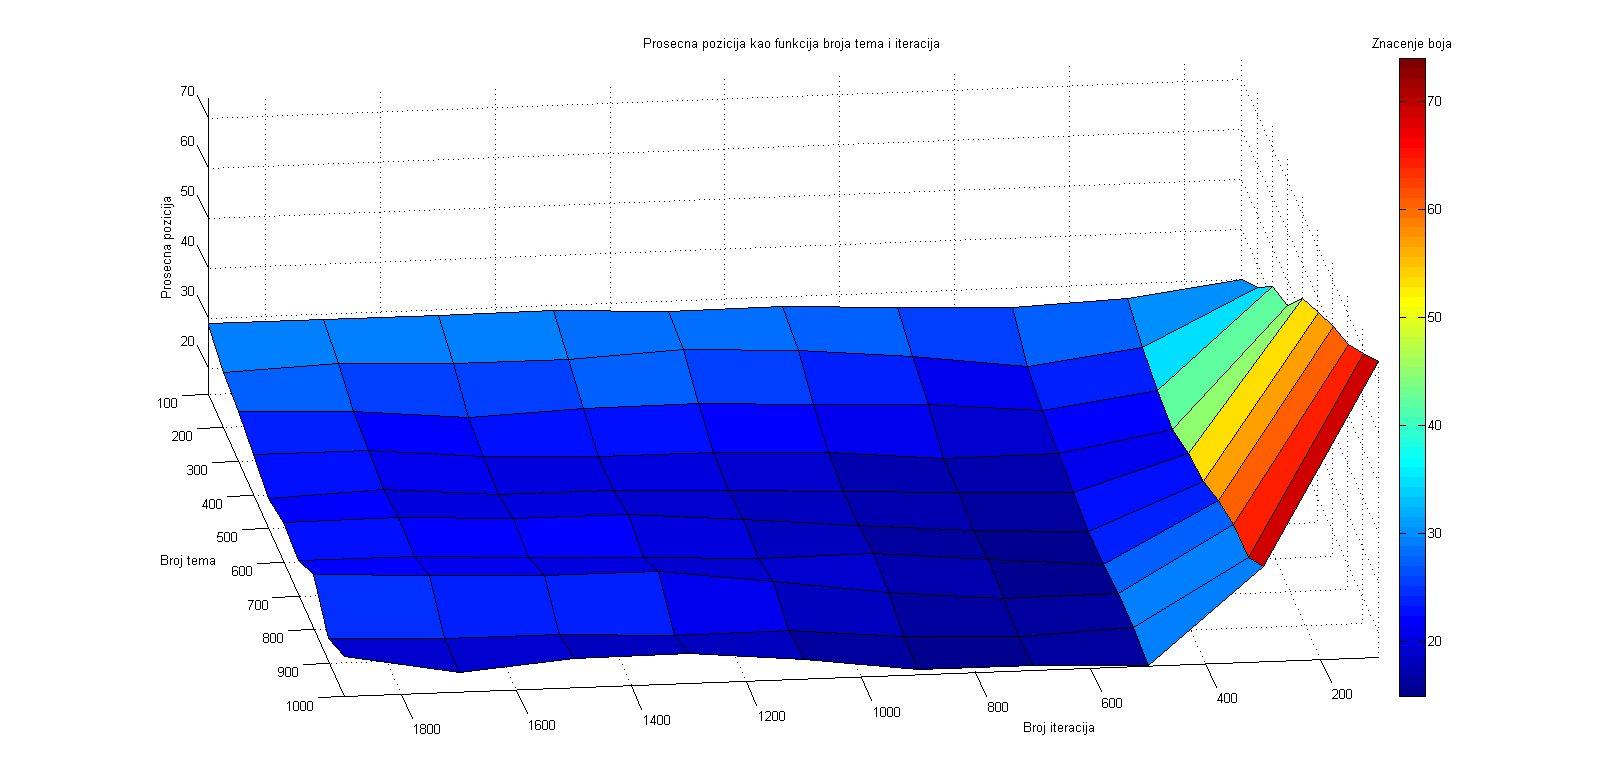
\includegraphics[scale=0.3]{./Slike/distNoStemSyn.png} 
	\caption{Зависност просечне позиције од броја тема и броја итерација}
	\label{fig:slika1}
\end{figure}

Минимална просечна позиција је \textbf{15} и добија се при више различитих комбинација параметара. Неке од комбинација су приказане у следећој табели

\begin{center}
\captionof{table}{Утицај броја тема и итерација на просечну позицију тачног одговора}
\begin{tabular}{|c|c|}
\hline
Број итерација & Број тема \\
\hline\hline
500 & 600 \\
500 & 700 \\
500 & 1000 \\
\hline
\end{tabular}

\end{center}





\subsection{Укупни резултати са синонимима и стемингом}

Поред поједничане примене сваке трансформације на улазне податке, у раду су тестиране и њихове комбинације. Обзором на то да стеминг уклања наставке, велики број тако модификованих добија нерегуларни облик. Због тога није могуће ни пронаћи њихове синониме. Да би се то избегло, најпре су додавани синоними за сваку реч а затим је извршен стеминг.

\subsubsection{Косинусна сличност}



Утицај  комбинације додавања синонима и стеминга на просечну позицију  када се сличност мери косинусном сличношћу дат је на следећем графику( слика 8.10)

		\begin{figure}[H]
    \centering
   \includegraphics[scale=0.3]{./Slike/StemmSyn.png} 
	\caption{Зависност просечне позиције од броја тема и броја итерација}
	\label{fig:slika1}
\end{figure}

Минимална просечна позиција је \textbf{10} и добија се при више различитих комбинација параметара. Неке од комбинација су приказане у следећој табели

\begin{center}
\captionof{table}{Утицај броја тема и итерација на просечну позицију тачног одговора}
\begin{tabular}{|c|c|}
\hline
Број итерација & Број тема \\
\hline\hline
500 & 555 \\
500 & 690 \\
500 & 712 \\
700 & 847 \\
\hline
\end{tabular}
\end{center}

Са графика је јасно да је утицај синонима значајан. Облик површи је јако сличан облику који се добија додавањем само синонима, без примене стеминга. Дакле, додавање синонима има јачи утицај од стеминга. Односно, додавање стеминг трансформације након убацивања синонима не утиче значајно на просечну позицију. 

\subsection{Укупни резултати са синонимима и лемитизацијом}

Још једна од комбинација улазних трансформација која је тестирана у овом раду је и комбинација лемитизација и синоними. Лемитизација ће свести речи на коренску, без обзира на облик те речи. Међутим, поред означавања времена и лица, различит облик речи може означавати и различито значење речи. Из тог разлога, најпре су додати синоними па је затим примењена лемитизација.

\subsubsection{Косинусна сличност}



Утицај  комбинације додавања синонима и лемитизације на просечну позицију  када се сличност мери косинусном сличношћу дат је на следећем графику( слика 8.11)


		\begin{figure}[H]
    \centering
   \includegraphics[scale=0.3]{./Slike/LemmSyn.png} 
	\caption{Зависност просечне позиције од броја тема и броја итерација}
	\label{fig:slika1}
\end{figure}

Минимална просечна позиција је \textbf{12} и добија се при тачно једној комбинацији параметара и то :

\begin{center}
\captionof{table}{Утицај броја тема и итерација на просечну позицију тачног одговора}
\begin{tabular}{|c|c|}
\hline
Број итерација & Број тема \\
\hline\hline
600 & 483 \\

\hline
\end{tabular}
\end{center}

Поново се примећује знатан утицај синонима на облик површи као и на просечну позицију. Лемитизација није значајно утицала на просечну позицију.



\subsubsection{Мерење сличности према лексичкој и тематској сличности}
	
Уколико се за меру сличности одабере мера  \textbf{лексичке и теметске} сличности, просечна позиција такође директно зависи од параметра модела. Обзиром на временску и просторну сложеност ове мере, нису испитиване све могућности за параметре модела. График зависности просечне позиције од броја тема и итерација дат јена следећој слици (слика 8.12)

		\begin{figure}[H]
    \centering
   \includegraphics[scale=0.3]{./Slike/distLemmSyn.png} 
	\caption{Зависност просечне позиције од броја тема и броја итерација}
	\label{fig:slika1}
\end{figure}

Минимална просечна позиција је \textbf{15} и добија се при више различитих комбинација параметара. Неке од комбинација су приказане у следећој табели

\begin{center}
\captionof{table}{Утицај броја тема и итерација на просечну позицију тачног одговора}
\begin{tabular}{|c|c|}
\hline
Број итерација & Број тема \\
\hline\hline
500 & 600 \\
500 & 700 \\
500 & 800 \\
\hline
\end{tabular}

\end{center}




\section{Упоредни резултати решења алгоритмом моделовања тема и бројањем речи}




\subsection{Косинусна сличност}

\begin{center}
\captionof{table}{Упоредни резултати алгоритме моделовања тема и решења бројањем речи}
\begin{tabular}{ | l | l | l | l | l || l | l | l | l | }
\hline
	 &\multicolumn{4}{|c||}{WC}  & \multicolumn{4}{|c|}{TM}  \\ \hline
	 & Prva & Top 10 & Top 20 & Top 30 & Prva & Top 10 & Top 20 & Top 30 \\ \hline
	noStemNoSyn & 231 & 324 & 339 & 343 & 179 & 288 & 308 & 324 \\ \hline
	stemNoSyn & 233 & 331 & 345 & 350 & 190 & 296 & 319 & 330 \\ \hline
	lemmNoSyn & 231 & 333 & 345 & 350 & 187 & 297 & 329 & 336 \\ \hline
	stemSyn & 177 & 319 & 337 & 342 & 147 & 282 & 304 & 324 \\ \hline
	lemmSyn & 175 & 312 & 335 & 342 & 146 & 280 & 309 & 322 \\ \hline
	noStemSyn & 175 & 309 & 335 & 339 & 147 & 286 & 305 & 325 \\ \hline
\end{tabular}
\end{center}

Из резултата се може уочити да се косинусном мером расподела тема по документима не могу добити бољи резултати од класичног приступа бројањем речи. Разлог за то може да буде недовољна количина података али и природа мера сличности. Обзором да се узима само тематска сличност, занемарује се јако битна карактеристика сличности два документа - лексичка.

Добијени резултати, обзором да се ради о малом скупу података, могу да наведу на закључак да постоји извесна зависност између дужине питања( одговора) и датих решења. 



\subsection{Мерење сличности према лексичкој и тематској сличности}

Обзиром на то да је ова сличност јако велике сложености, из практичних разлога, нису тестиране све трансформације. Резултати који су добијени дати су у следећој табели:

\begin{center}
\captionof{table}{Упоредни резултати алгоритме моделовања тема и решења бројањем речи}
\begin{tabular}{ | l | l | l | l | l || l | l | l | l | }
\hline
	 &\multicolumn{4}{|c||}{WC}  & \multicolumn{4}{|c|}{TM}  \\ \hline
	 & 0 & 10 & 20 & 30 & 0 & 10 & 20 & 30 \\ \hline
	noStemNoSyn & 231 & 324 & 339 & 343 & 217 & 308 & 332 & 340 \\ \hline
	stemNoSyn & 233 & 331 & 345 & 350 & 215 & 325 & 339 & 343 \\ \hline
	lemmNoSynEnd & 231 & 333 & 345 & 350 & 213-232 & 319 & 338 & 342 \\ \hline
	lemmSyn & 175 & 312 & 335 & 342 & 150 & 270 & 288 & 304 \\ \hline
\end{tabular}
\end{center}


Дакле, ова мера показује незнатно слабије резултате од класичног метода, стим што јој је комплекснонст знатно већа. Са друге стране, добијена прецизност решења је већа него код косинусне сличности.Међутим, како је потребно доста времена да би се добили резултати, ова мера није даље разматрана. 

\subsection{Сличност према предвиђеној вероватноћи}

Полазни тестни скуп има 360 питања и 360 одговора. Он је довољно мали да омогућава тестирање сваке од поменутих мера, довољно велики да би се уочили трендови али недовољан да би се донели генерални закључци. 

Обзиром на то да је ова мера  показала најбоље резултате, поред стандардног тестног скупа, тестирана је и на већим скуповима података. Величине додатних скупова података су по 200, 800, 1400, 2000, 10000, 20000 и 40000 докумената, односно 100, 400, 700, 1000, 5000, 10000 и 20000 питања и исто толико одговора. Подаци су преузети са сајта \textit{answers.yahoo.com}

Ова додатна тестирања су била неопходна како би се избегао енг. overfitting, тј. како би се донели закључци који што мање зависе од података. 

Енг. overfitting је термин машинског учења који се односии на прилагођавање програма подацима. Тада се најчешће дешава да програм  са изузетно великом прецизношћу  ради са једним скупом података, док са другим скупом та прецизност драстично опада. Разлог томе је што је програм \textbf{научен} да ради само са одређеним скупом података .
У конкретном случају, немогуће је потпуно побећи од енг. overfitting-а због природе проблема. Међутим, уколико се покаже да модели грађени над различитим скупом података показују исте особине, тада се могу извести закључци који су релативно независни од података. 
 

Компаративни модел, као и досада било је решење бројањем речи. Резултати добијени мерењем дати су у следећој табели :
\begin{table}[H]
\centering
\caption{Упоредни резултати решења алгоритма моделовања тема употребом мере сличности на основу предвиђене вероватноће и компаративног решења}
\begin{tabular}{ | l | l | l | l | l || l | l | l | l | l | }
\hline
	 & \multicolumn{4}{|c||}{WC}  & \multicolumn{5}{|c|}{TM}  \\ \hline
	Broj dokumenata & Prva & Top 10 & Top 20 & Top 30 & Prva & Top 10 & Top 20 & Top 30 &  Br. tema \\ \hline
	100 & 72 & 90 & 91 & 91 & 66 & 87 & 91 & 94 & 50 \\ \hline
	400 & 203 & 338 & 353 & 361 & 217 & 326 & 336 & 348 & 400 \\ \hline
	700 & 338 & 569 & 596 & 610 & 357 & 546 & 583 & 594 & 750 \\ \hline
	1000 & 453 & 789 & 836 & 853 & 472 & 744 & 794 & 829 & 1100 \\ \hline
	5000 & 1484 & 3002 & 3367 & 3570 & 1614 & 2960 & 3279 & 3472 & 800 \\ \hline
	10000 & 2422 & 5334 & 6054 & 6521 & 2766 & 5297 & 5988 & 6421 & 1100 \\ \hline
	20000 & 3866 & 9044 & 10516 & 11460 & 4576 & 9182 & 10546 & 11358 & 900 \\ \hline
\end{tabular}
\end{table}

Као што се може приметити, алгоритам моделовања тема готово увек успева да на прву позицију избаци више тачних одговора него компаративно решење. Једино за  улазни скуп од 100 питања и 100 одговора ово није испуњено, иако не одступа много. Може бити више разлога за овакво понашање:
\begin{itemize}
\item Природа података које погодује компаративном решењу
\item Недовољна количина података - модел  нема довољно информација
\end{itemize}

Даље испитивање узрока оваквог понашања није од интереса. Пре свега, улазни скуп је јако мали, тако да резултати доста зависе од података. Са друге стране, ова величина скупа је недовољна за било какву реалну примену.

Уколико се графички представи број докумената који се појављују на првој позицију у односу на величину улазног скупа, може се приметити да са повећањем улазних података, разлика у резултатима ова два решења постаје већа. Графички приказ дат је на следећој слици :

\begin{figure}[H]
  \centering
   \includegraphics[scale=0.8]{./Slike/prvePoz.png} 
	\caption{Прва позиција у односу на величину улазног скупа}
	\label{fig:slika1}
\end{figure}

Појављивање тачног одговора на првој позицији може бити престрог критеријум за упоређивање резултате ове две методе. Стога се поред прве позиције, за меру оцене може узети и појављивање тачног одговора у првих 10 предложених резултата. Графички приказ резултата поменуте две методе дат је на следећој слици.

\begin{figure}[H]
  \centering
   \includegraphics[scale=0.8]{./Slike/top10.png} 
	\caption{Број тачних одговора у првих 10 предложених резултата у односу на величину улазног скупа}
	\label{fig:slika1}
\end{figure}

Као што се може уочити са слике, резултати ове две методе мерене са становишта првих 10 предложених резултата, готово се идентично понашају. 



Поред броја тачнох одговора који се налазе на првој позицији, или у првих 10 предложених одговора, важна карактериста оба решења је \textbf{прецизност}. Под прецизношћу решења подразумева се \textbf{проценат} тачних одговора који испуњавају неки критеријум. У конкретном случају, од интереса је да ли се налазе на првој позицији, односно да ли се налазе у првих 10 предложених решења.

Прецизност оба решења у односу на то да ли се тачан одговор појављује на првој позицији у листи предложених одговора дат је на следећој слици :

\begin{figure}[H]
  \centering
   \includegraphics[scale=0.8]{./Slike/procenatPrva.png} 
	\caption{Прецизност предложених решења}
	\label{fig:slika1}
\end{figure}

Са слике се може закључити следеће :
\begin{itemize}
\item Оба решења губе прецизност са повећањем броја улазних података
\item Прецизност решења алгоритмом моделовања тема спорије опада него прецизност решења бројањем речи
\item Разлика у прецизности ова два решења повећава се са повећањем броја улазних података
\end{itemize}

Упоредна прецизност предложених решења у односу на то да ли се тачан одговор налази у првих 10 предложених одговора, дата је на следећем графику :

\begin{figure}[H]
  \centering
   \includegraphics[scale=0.8]{./Slike/procenat10.png} 
	\caption{Прецизност предложених решења}
	\label{fig:slika1}
\end{figure}

Могу се извести слични закључци као и за прецизност везану за појављивање тачног одговора на првој позицији :

\begin{itemize}
\item Са порастом величине улазних података, прецизност оба решења опада
\item Прецизност решења бројањем речи је већа него прецизност решења моделовањем тема за величину улазнпог скупа до 5000. Након тога, прецизности оба решења су готово исте.
\end{itemize}


\textbf{Статистичка значајност разлике у резултатима}\\

Како би изведени закључци били поузданији, урађени су и статистички тестови значајности над добијеним резултатима. У конкретном случају рађен је Вилкоксонов тест за упоредне резултате добијене на првој позицији оба решења. Овим тестом се испитује  да ли постоји статистички значајна разлика у резултатима ове две методе. Услов значајности је да сигнификантност добијена овим тестом буде $<0.05$. Резултати тестова налазе се у следећој табели :
\begin{table}[H]
\centering
\caption{Резултати Вилкоксоновог теста}

\begin{tabular}{ | l | l | l | l | l | }
\hline
	
	Broj dokumenata & Prva WC & Prva TM & Signifikantnost & Značajno \\ \hline
	100 & 72 & 66 & 0.71099999999999997 & NE \\ \hline
	400 & 203 & 217 & 3.1E-2 & DA \\ \hline
	700 & 338 & 357 & 2.1000000000000001E-2 & DA \\ \hline
	1000 & 453 & 472 & 2E-3 & DA \\ \hline
	5000 & 1484 & 1614 & 7.4999999999999997E-2 & NE \\ \hline
	10000 & 2422 & 2766 & 2.7E-2 & DA \\ \hline
	20000 & 3866 & 4576 & 0 & DA \\ \hline
	
\end{tabular}

\end{table}

На основу резултата у претходној табели, може се закључити да разлике у мерењима нису случајне већ зависне од метода. При тестирању резултата на скупу од 5000 одговора, утврђено је да разлике између метода нису статистички значајне. Ово не мора да значи да разлике између метода не постоје. Праг значајности са којим су рађени тестови је 0.05, док је сигнификантност добијена у овом скупу података 0.07. Ова мала разлика може да буде последица од грешке у рачуну ( нагомилана грешка ) до специфичности података.  
%\chapter{Коришћене скраћенице}
\begin{enumerate}
\item енг. - енглески језик
\item срп. - српски језик
\item LDA - Latent Dirichlet Allocation
\item TM - Topic Model, срп. моделовање тема
\end{enumerate}
\chapter{Додатак}

\section{Предпроцесирање}

\begin{lstlisting}

public class PipeStem extends Pipe{

	private static final long serialVersionUID = 1L;

	public Instance pipe(Instance carrier) {	
		 SnowballStemmer stemmer = new englishStemmer();
		 TokenSequence in = (TokenSequence) carrier.getData();

		 for (Token token : in) {
		 stemmer.setCurrent(token.getText());
		 stemmer.stem();
		 token.setText(stemmer.getCurrent());
		 }

		 return carrier;
		 }

}

\end{lstlisting}


\begin{lstlisting}


public class StanfordLemmatizer extends Pipe{

    protected StanfordCoreNLP pipeline;

    public StanfordLemmatizer() {
         Properties props;
         props = new Properties();
         props.put("annotators", "tokenize, ssplit, pos, lemma");

         this.pipeline = new StanfordCoreNLP(props);
     }

public Instance pipe(Instance carrier) {	
	
	 TokenSequence in = (TokenSequence) carrier.getData();

	 for (Token token : in) {
	 String text = lemmatize(token.getText());
	 token.setText(text);
	 }

	 return carrier;
	 }
	
    public String lemmatize(String documentText)
    {
        List<String> lemmas = new LinkedList<String>();
         Annotation document = new Annotation(documentText);
         this.pipeline.annotate(document);
        List<CoreMap> sentences = document.get(SentencesAnnotation.class);
        String lemmasString = "";
        for(CoreMap sentence: sentences) {
             for (CoreLabel token: sentence.get(TokensAnnotation.class)) {
                  lemmasString+=token.get(LemmaAnnotation.class);
            }
        }
        return lemmasString;
    }


   
}


\end{lstlisting}

\section{Оптималан број тема и итерација}

\begin{lstlisting}

for i in `seq 100 200 2000` 
do
	qsub -v topic=500,iter=$i job.sub	
done

\end{lstlisting}

job.sub	:

\begin{lstlisting}

	 java -Xms6000m -Xmx10000m -classpath "/lustre/home/jvasiljevic/TopicModeling/Mallet/class:/lustre/home/jvasiljevic/TopicModeling/Mallet/lib/mallet-deps.jar:/lustre/home/jvasiljevic/TopicModeling/Mallet/lib/jdom-1.0.jar:/lustre/home/jvasiljevic/TopicModeling/Mallet/lib/grmm-deps.jar:/lustre/home/jvasiljevic/TopicModeling/Mallet/lib/weka.jar:jaws-bin.jar:./stanford-lemmitization/stanford-corenlp-3.5.2.jar:./stanford-lemmitization/stanford-corenlp-3.5.2-models.jar:." -Dwordnet.database.dir=/usr/share/wordnet-3.0/dict/  TestFixParamKlaster ../../odgovor1.csv ../../pitanje1.csv $lambda $mi ../../Mallet/stoplists/stopwords.txt
	 
	 
\end{lstlisting}





\section{Мерење сличности}

\begin{lstlisting}

	public static double dotProd(double[] a, double[] b){
		if(a.length != b.length){
			throw new IllegalArgumentException("The dimensions have to be equal!");
		}
		double sum = 0;
		for(int i = 0; i < a.length; i++){
			sum += a[i] * b[i];
		}
		return sum;
	}
	public static double intensity(double[] a)
	{
		double sum = 0;
	
		for(int i = 0; i < a.length; i++){
			sum+= a[i]*a[i];
		}
		
		return Math.sqrt(sum);
	}
	


	
	public static double cosineSim(double[] broj1,double[] broj2)
	{
		return dotProd(broj1, broj2)/(intensity(broj1)*intensity(broj2));// *intensityOdg(broj2,broj1));
	}
\end{lstlisting}


%
% Spisak Literature
%
\begin{thebibliography}{11}
\bibitem{larsv} {Lars Vogel, Android Service and Broadcast Receiver, www.vogella.de, 2011.}
\bibitem{blei1} { David M. Blei,Introduction to Probabilistic Topic Models,Princeton University}
\bibitem{blei2} { David M. Blei, Topic Models,Princeton University,September 1,2009}
\bibitem{mimno1} { David Mimno,The details: training	and validating big	models on big data,Princeton University}
\bibitem{verov1} {Ivana Kovačević, Verovatnoća i statistika sa zbirkom zadataka, Beograd 2011.}
\bibitem{verov2} {Violeta Aleksić, Elementi teorije verovatnoće i matematičke statistike, }
\bibitem{verov3} {www.ekfak.kg.ac.rs, kurs Osnovi statistike, avgust 2015.}
\bibitem{verov4} {http://starisajt.elfak.ni.ac.rs/phptest/new/html/Studije/predavanja-literatura/matematika-odabrana-poglavlja/verovatnoca.pdf, avgust 2015}
\bibitem{verov5} {Random Signals and Processes Primer with MATLAB, Gordana Jovanovic Dolocek,2013}
\bibitem{verov6} {Lecture 32: Markov Chains Continued | Statistics 110  on youtube - https://www.youtube.com/watch?v=aBGOyZv2pZE, avgust 2015}
\bibitem{verov6} {Christopher M. Bishop, Pattern Recognition and
Machine Learning, Springer, 2006}
\bibitem{verov7} {http://fourier.eng.hmc.edu/e161/lectures/gaussianprocess/node7.html, avgust 2015}
\bibitem{verov8} {https://theclevermachine.wordpress.com/2012/11/05/mcmc-the-gibbs-sampler/, avgust 2015}
\bibitem{verov9} {William M. Darling, A Theoretical and Practical Implementation Tutorial on Topic Modeling and Gibbs Sampling, December 1, 2011}
\bibitem{verov10} {Yi Wang, Distributed Gibbs Sampling of Latent Topic Models: The Gritty Details, August , 2008}
\end{thebibliography}

\pagebreak

\thispagestyle{empty}

\leftline{УНИВЕРЗИТЕТ У КРАГУЈЕВЦУ}

\leftline{ПРИРОДНО-МАТЕМАТИЧКИ ФАКУЛТЕТ}


\leftline{ИНСТИТУТ ЗА МАТЕМАТИКУ И ИНФОРМАТИКУ}

\vspace*{2cm}

Завршни рад под називом \vspace*{3mm}

% \centerline{Uneti ovde naziv zavrsnog rada} 
\vspace*{3mm}

\noindent одбрањен је \rule{3cm}{0.5pt}.
\vspace*{2cm}


\noindent МЕНТОР:
\vspace*{1cm}

\noindent \rule{7cm}{0.5pt}

\noindent др Име Презиме, звање, Институција
\vspace*{2cm}

 

{\phantom{a}\hfill ЧЛАНОВИ
КОМИСИЈЕ:\qquad\qquad\qquad}
\vspace*{1cm}

\noindent\hspace*{6cm}\rule{7cm}{0.5pt}

\noindent\hspace*{6cm} др Име Презиме, звање, Институција
\vspace*{1cm}

\noindent\hspace*{6cm}\rule{7cm}{0.5pt}

\noindent\hspace*{6cm} др Име Презиме, звање, Институција

\vspace*{2cm}

Завршни рад је оцењен оценом \rule{3cm}{0.5pt}.


\end{document}


